\documentclass[twoside]{article}
\usepackage{graphicx}
\usepackage[margin=4cm]{geometry}
\usepackage{calligra}
\usepackage[colorlinks, linkcolor=azulsema!60!black]{hyperref}
\usepackage{wrapfig}
\usepackage{multicol}
\usepackage{subfigure}
\usepackage{eurosym}
%\usepackage[latin1]{inputenc}
\usepackage[utf8]{inputenc}
\usepackage[T1]{fontenc}
\usepackage[spanish]{babel}
\usepackage{colortbl}
\usepackage{float}
\usepackage{tikz}
%\DeclareGraphicsExtensions{.png,.pdf,.jpg,.gif}
\usetikzlibrary{babel,calc,intersections,through,backgrounds,shadings,fadings}

\definecolor{azulsema}{cmyk}{0.83, 0.3, 0.18, 0.11}
\definecolor{azulcielo}{cmyk}{0.69, 0.42, 0.11, 0.03}

\begin{document}
\shorthandoff{>}\shorthandoff{<} %Necesario para compatibilizar los paquetes [spanish]{babel} 

\section{7th European Workshop on High Order Nonlinear Numerical Methods for Evolutionary PDEs: Theory and Applications, HONOM 2019, 1-5 abril 2019, Madrid}

\begin{center}\large
\textbf{Arturo Hidalgo}\\
Escuela Técnica Superior de Ingenieros de Minas y Energía. Universidad Politécnica de Madrid.  \\
{\color{azulsema}\rule{.5\linewidth}{1pt}}
\end{center}
La séptima edición del congreso European Workshop on High Order Nonlinear Numerical Methods for Evolutionary PDEs: Theory and Applications (HONOM 2019) se celebró en la Escuela Técnica Superior de Ingenieros de Minas y Energía (ETSIME) de la Universidad Politécnica de Madrid, entre los días $1$ y $5$ de abril de $2019$. La temática del congreso está relacionada con métodos de simulación numérica de alto orden para la resolución de gran variedad de problemas no lineales que se presentan, de manera muy especial, en el ámbito de la mecánica de fluidos, pero también en muchos otros, como el cálculo de estructuras, la magnetohidrodinámica, fusión nuclear o aplicaciones biomédicas. Los métodos numéricos que se utilizan en tales aplicaciones están basados fundamentalmente en volúmenes finitos, Galerkin discontinuo y elementos finitos. Las ediciones anteriores de HONOM se han celebrado en Trento ($2007$, $2009$, $2011$, $2015$), Burdeos ($2013$) y Stuttgart ($2017$). 

El Comité Organizador de HONOM está formado por los profesores Eleuterio Toro (Universidad de Trento), Rémi Abgrall (Universidad de Zurich), Michael Dumbser (Universidad de Trento) y Claus-Dieter Munz (Universidad de Stuttgart), mientras que el Comité Organizador Local de la reciente edición ha estado constituido por los profesores de la Universidad Politécnica de Madrid: Arturo Hidalgo (en calidad de Presidente del Comité Organizador Local), José Luis Parra (director de la E.T.S.I. de Minas y Energía), Carlos Conde, Francisco Javier Elorza, Alfredo López y Lourdes Tello. Se habilitó una página web que se utilizó tanto para información sobre el congreso, como para realizar la inscripción en el mismo, publicar los resúmenes de las comunicaciones y, en general, de interacción entre los organizadores y los participantes. La dirección de la página es:
http://eventos.upm.es/go/honom2019.

Las contribuciones al congreso se estructuraron en conferencias plenarias y comunicaciones orales. La mayor parte de estas últimas se desarrolló en sesiones paralelas. Cada jornada se abría en sesión de mañana con una conferencia plenaria, en el Salón de Actos de la Escuela, de una hora de duración, que daba paso a una de las comunicaciones orales, que tenía asignado un tiempo de exposición de media hora. Esta presentación tenía lugar también en el Salón de Actos. A continuación se desarrollaban las sesiones paralelas, donde las contribuciones orales tenían asignadas también media hora. Las salas donde se desarrollaban las sesiones paralelas eran el Salón de Actos y el aula Fausto de Elhuyar. La sesión de tarde se abría también con una conferencia plenaria que, posteriormente, daba paso a las sesiones paralelas.

El número de comunicaciones orales presentadas fue de $53$. Tanto las comunicaciones como las conferencias invitadas fueron de un muy elevado nivel científico. Es interesante destacar también que, además de profesores y científicos de reconocido prestigio internacional, hubo bastantes conferenciantes jóvenes que están iniciando su carrera investigadora. Los participantes procedían de $12$ países diferentes. Una selección de las comunicaciones presentadas se publicará en un número especial de la revista Communications on Applied Mathematics and Computation (CAMC), de la editorial Springer, denominado 'High order numerical methods for evolutionary PDEs', cuyo editor jefe es Chi-Wang Shu y los editores invitados son Rémi Abgrall, Michael Dumbser, Claus-Dieter Munz, Eleuterio F. Toro, Jan Hesthaven y Arturo Hidalgo.

La inauguración del congreso tuvo lugar el $1$ de abril, a las 9:30 horas en el Salón de Actos de la Escuela. La mesa presidencial estuvo formada por los profesores José Luis Parra, Eleuterio Toro, y Arturo Hidalgo. Fue un acto breve, en el que se dio la bienvenida a los asistentes al congreso.
%
\begin{center}
\begin{figure}
	\centering
		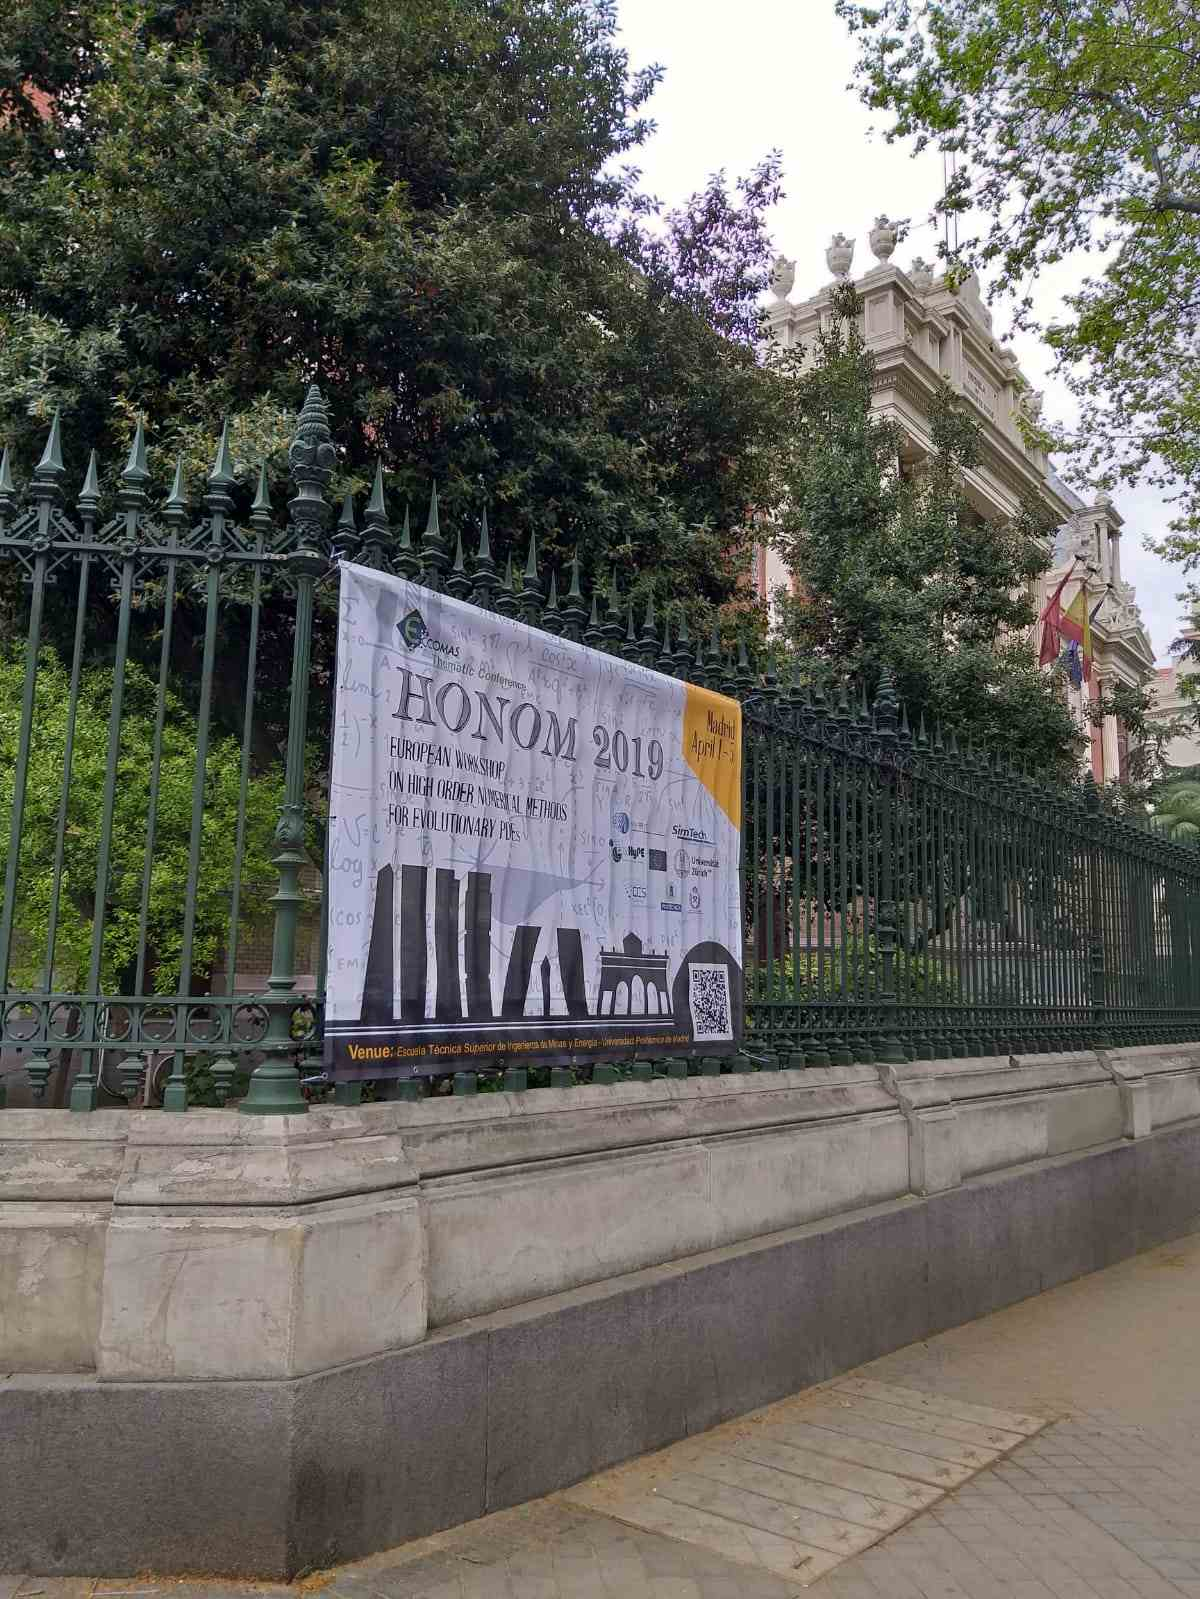
\includegraphics[width=.75\textwidth]{Lona}
	\label{fig:LonaVerja}
	\caption{Lona anunciadora de HONOM 2019 en la verja de ETSI de Minas y Energía  - Fuente: Comité Organizador}
\end{figure}
\end{center}
%
\begin{center}
\begin{figure}
	\centering
		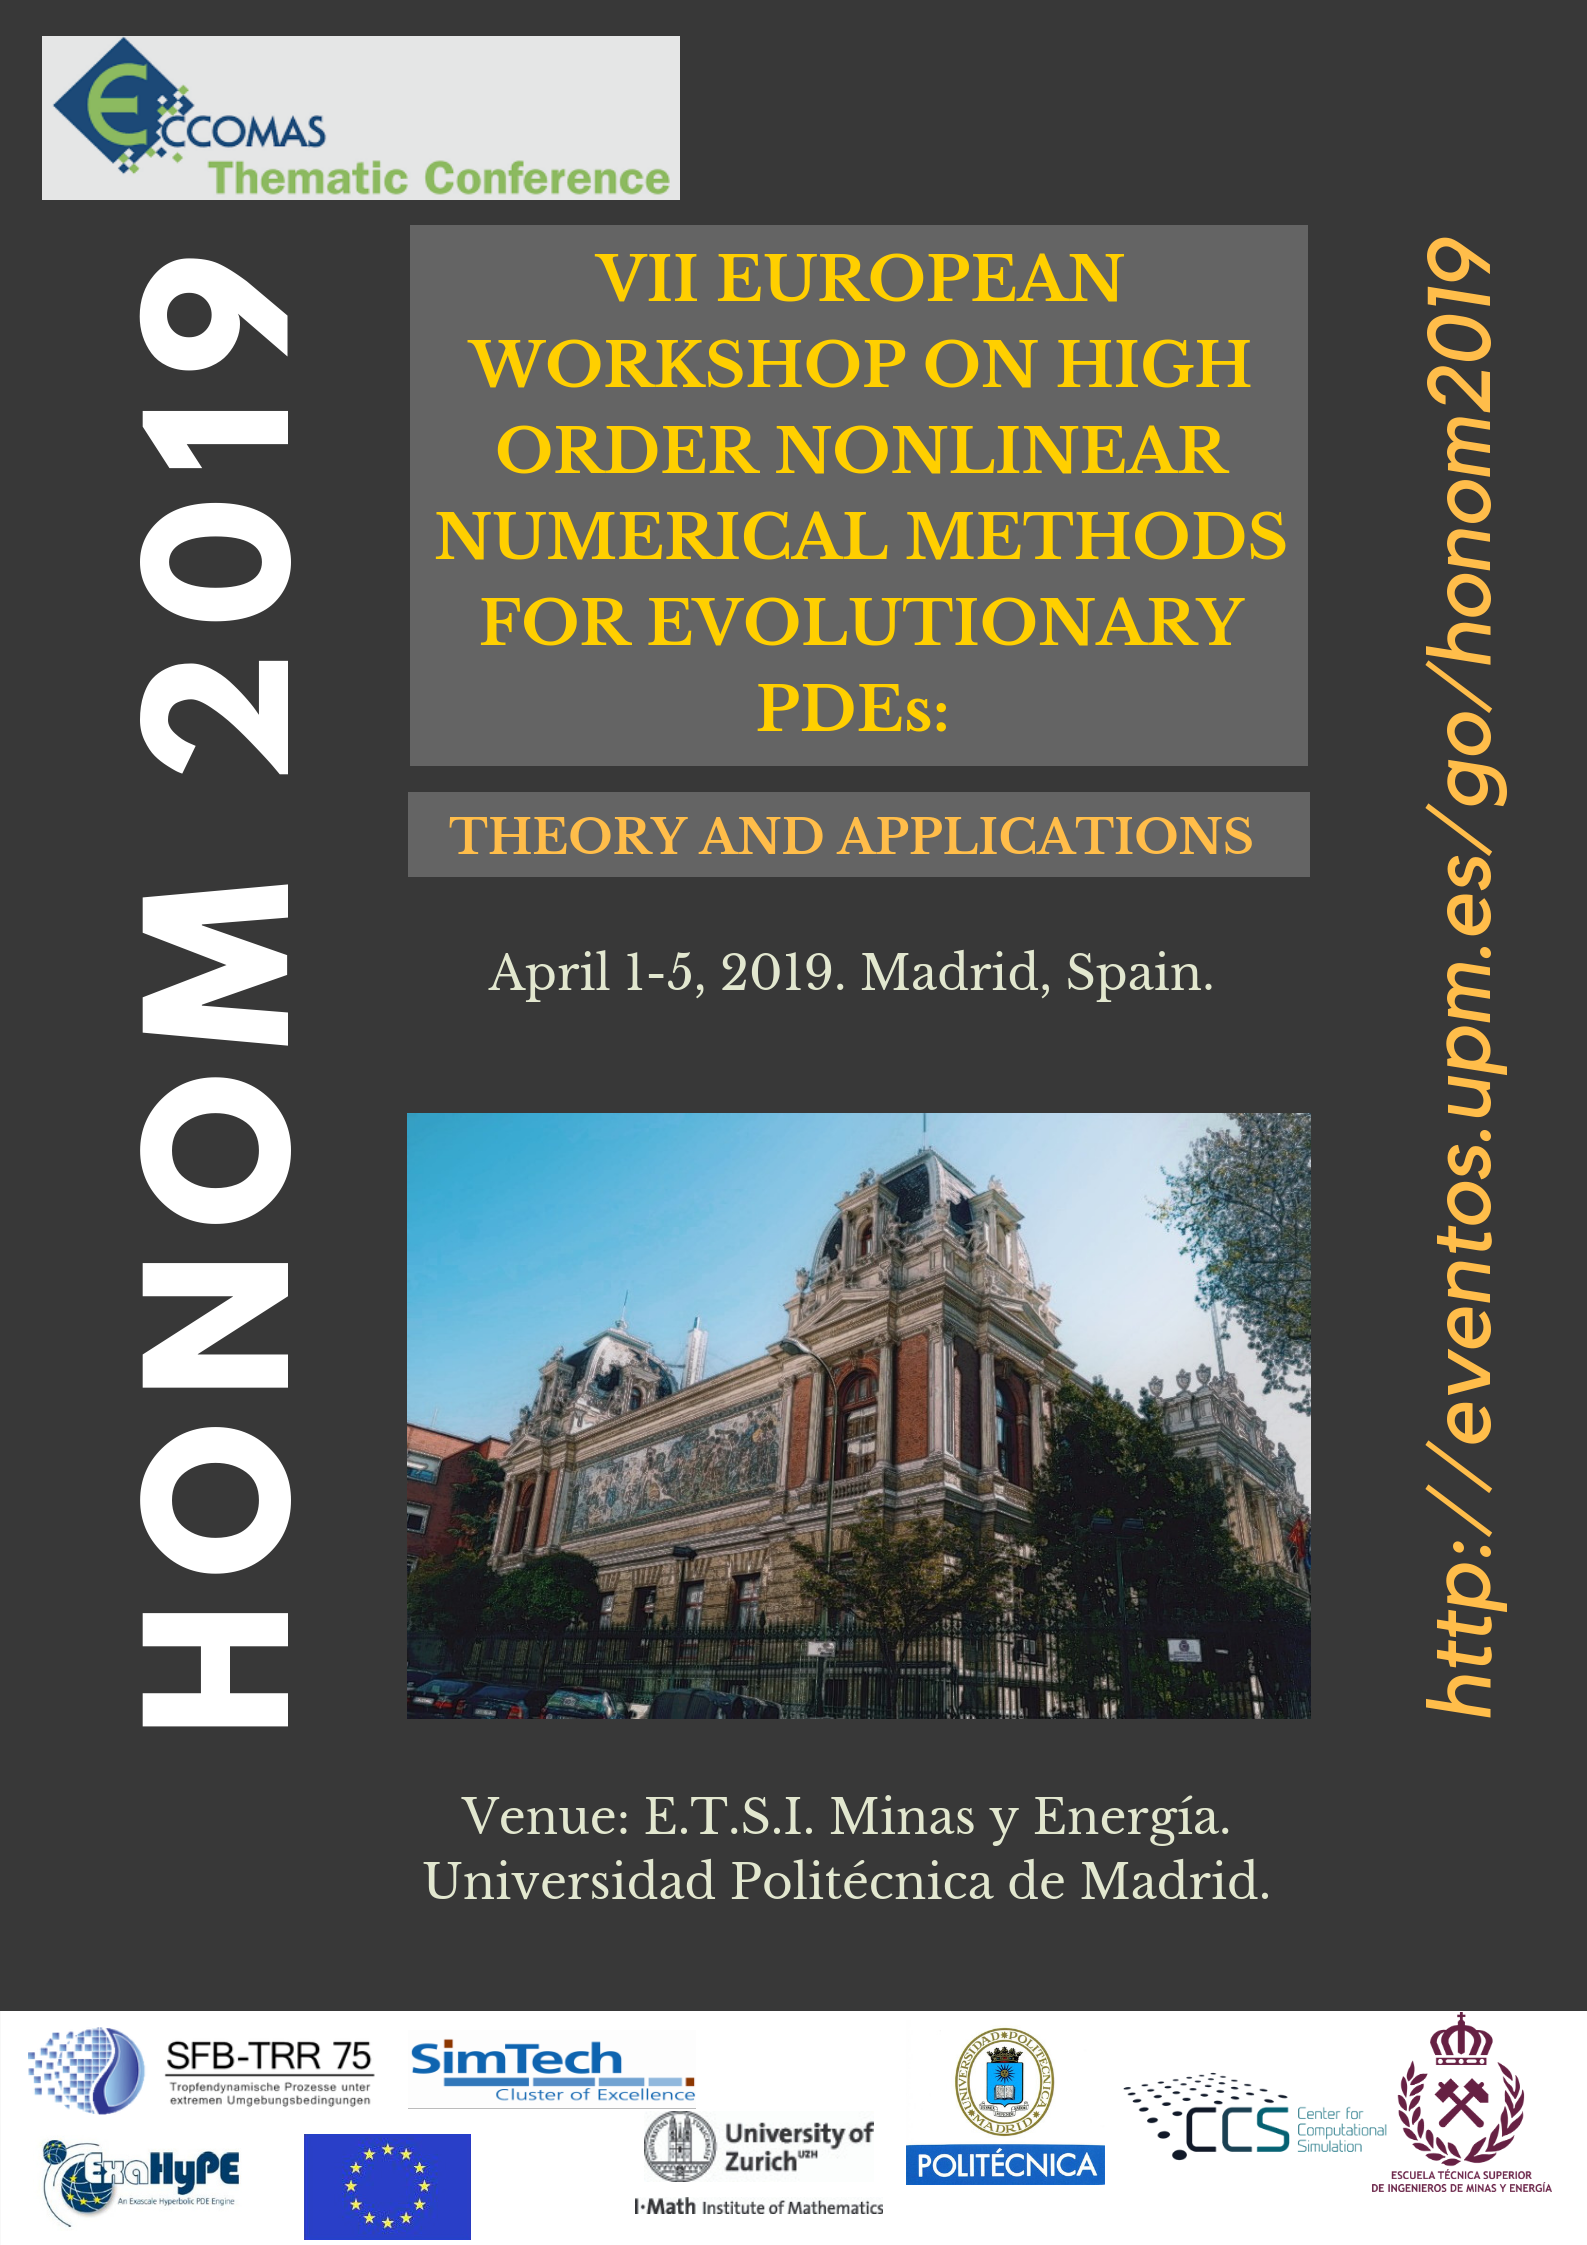
\includegraphics[width=.85\textwidth]{Poster_HONOM2019}
	\label{fig:Cartel}
	\caption{Cartel anunciador de HONOM 2019  - Fuente: Comité Organizador}
\end{figure}
\end{center}
%
\begin{center}
\begin{figure}
	\centering
		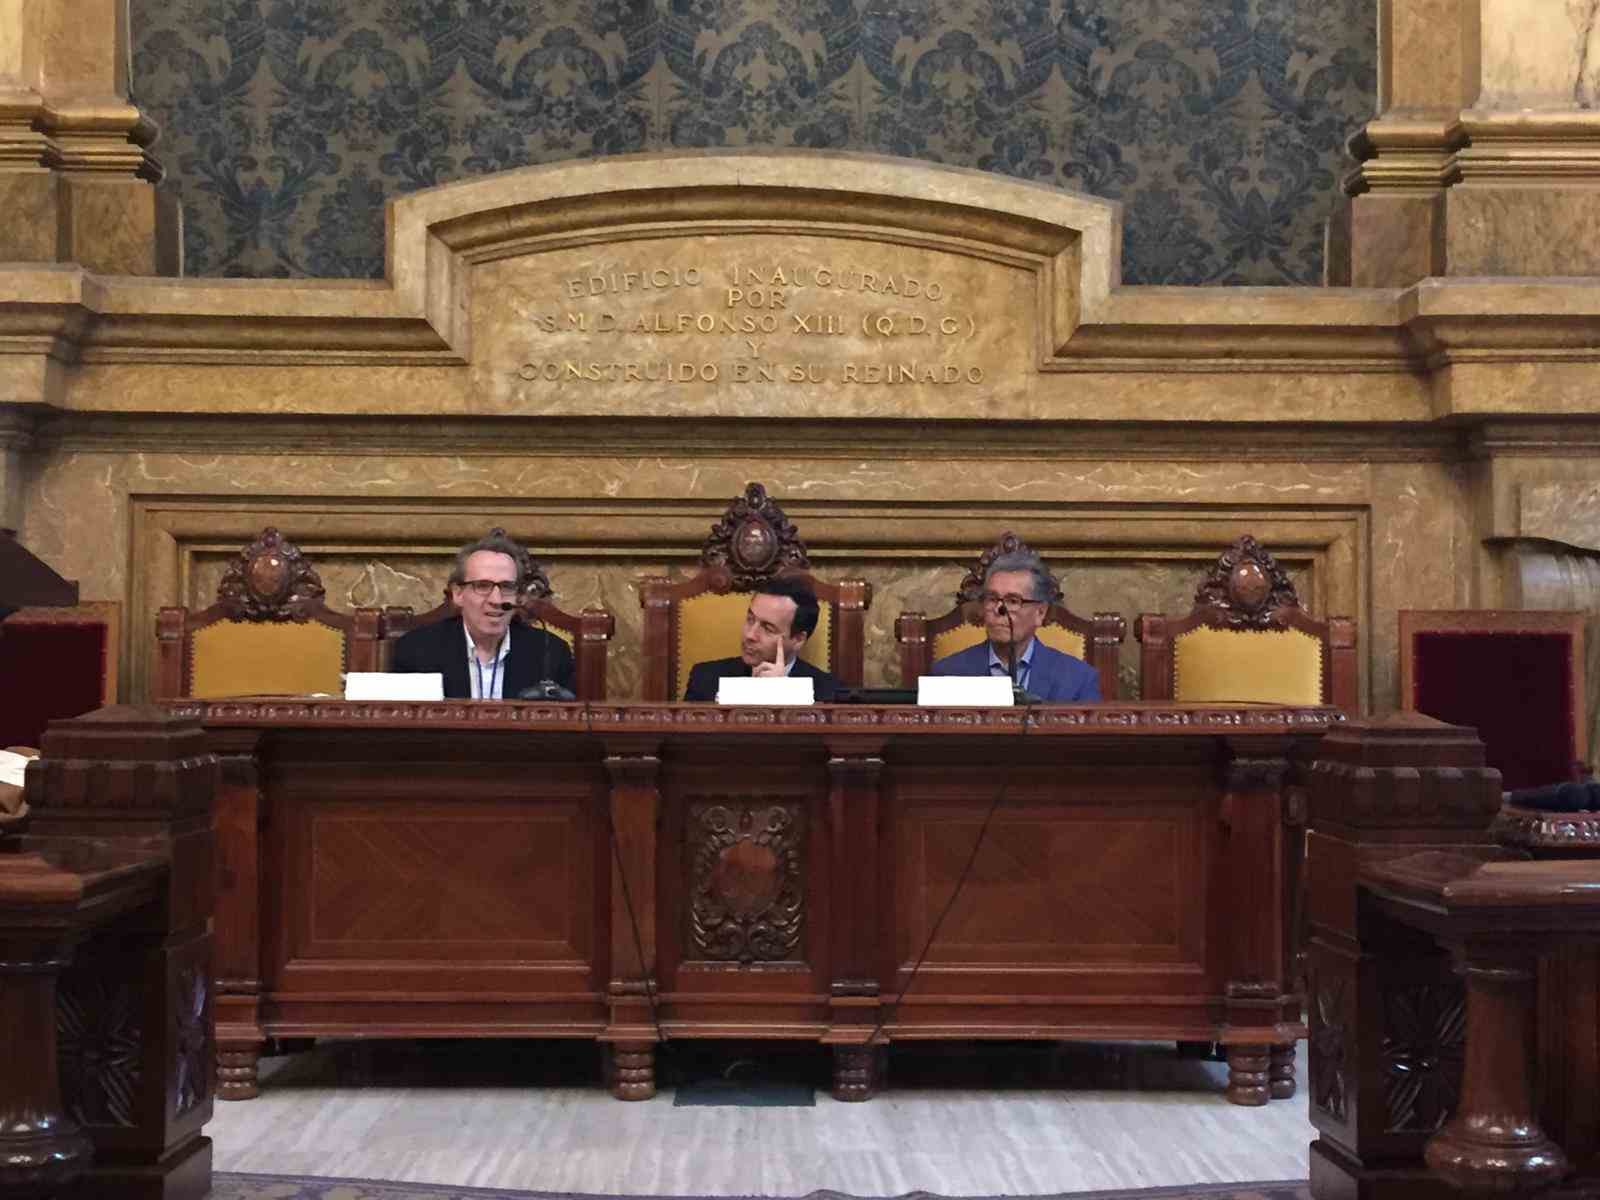
\includegraphics[width=.95\textwidth]{Mesa}
	\label{fig:MesaP}
	\caption{Mesa presidencial de la jornada inaugural de HONOM 2019. De derecha a izquierda Eleuterio F. Toro (Comité Organizador), José Luis Parra (Director de la ETSI de Minas y Energía) y Arturo Hidalgo (Presidente del Comité Organizador Local) - Fuente: Comité Organizador}
\end{figure}
\end{center}

\begin{center}
\begin{figure}
	\centering
		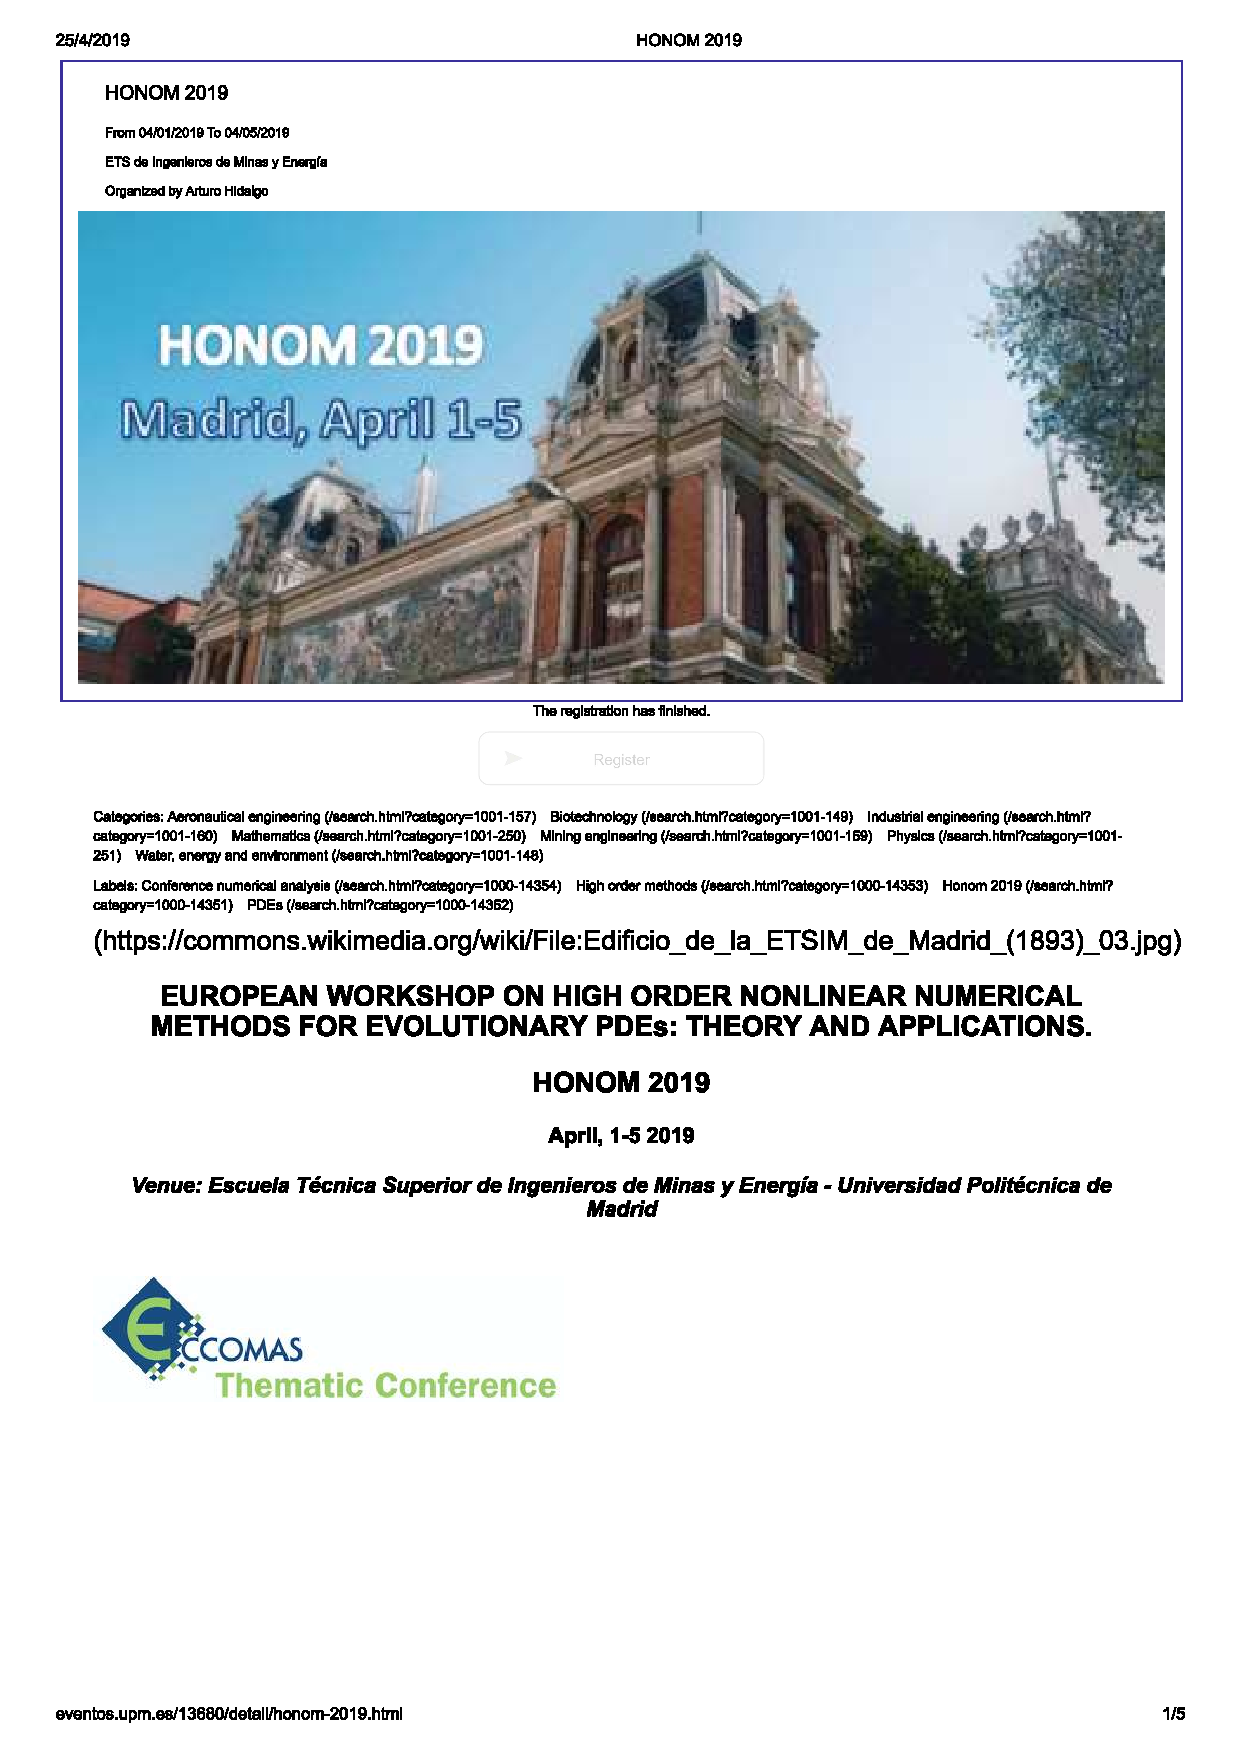
\includegraphics[width=.85\textwidth]{Web}
	\label{fig:WebFront}
	\caption{Portada de la página web. http://eventos.upm.es/go/honom2019  - Fuente: Comité Organizador}
\end{figure}
\end{center}

\subsection{Conferenciantes plenarios}

El congreso contó con nueve conferenciantes plenarios: Jan Hesthaven (École Polytechnique Fédérale de Lausanne, Suiza), Raphael Loubère	(Université de Bordeaux, Francia), Pep Mulet	(Universitat de Valencia, España), Ilya Peshkov	(Université Paul Sabatier,Toulouse III, Francia), Gabriella Puppo	(Università degli Studi dell'Insubria, Italia), Vladimir Titarev	(Federal Research Center Computer Science and Control, Rusia), Svetlana Tokareva	(Los Alamos National Laboratory, EE.UU.), María Elena Vázquez-Cendón	(Universidade de Santiago de Compostela, España) y Helen Yee	(NASA Ames Research Center, EE.UU.). Estas conferencias se distribuyeron de la siguiente manera:

\begin{itemize}
	\item Pep Mulet. \textit{Implicit-explicit schemes for degenerate diffusion-convection PDE}. Lunes 1 de abril de 10:00 a 11:00.
	\item Ilya Peshkov. \textit{The need for structure preserving methods in continuum physics}. Lunes 1 de abril de 14:30 a 15:30.
	\item Raphaël Loubère. \textit{A posteriori cures of inherent numerical issues generated by high accurate schemes}. Martes 2 de abril de 9:00 a 10:00.
	\item Gabriella Puppo. \textit{High order well balanced methods for gas dynamics with gravity}. Martes 2 de abril de 14:30 a 15:30.
	\item María Elena Vázquez Cendón. \textit{Well-balanced finite volume segregated schemes for hyperbolic non linear systems with source terms}. Miércoles 3 de abril de 9:00 a 10:00.
	\item Helen Yee. \textit{Two Decades Old Entropy Stable Methods for the Euler Equations Revisited}. Miércoles 3 de abril de 14:30 a 15:30.
	\item Jan Hesthaven. \textit{Controlling oscillations in high-order accurate methods through neural networks}. Jueves 4 de abril de 9:00 a 10:00.
	\item Vladimir Titarev. \textit{Numerical analysis of high-speed three-dimensional flows of rarefied gas on the basis of the Shakhov model}. Jueves 4 de abril de 14:30 a 15:30.
	\item Svetlana Tokareva. \textit{Advances in High-order Residual Distribution Scheme for Fluid Dynamics and Lagrangian Hydrodynamics}. Viernes 5 de abril de 9:00 a 10:00.
\end{itemize}
%
\begin{center}
\begin{figure}
	\centering
		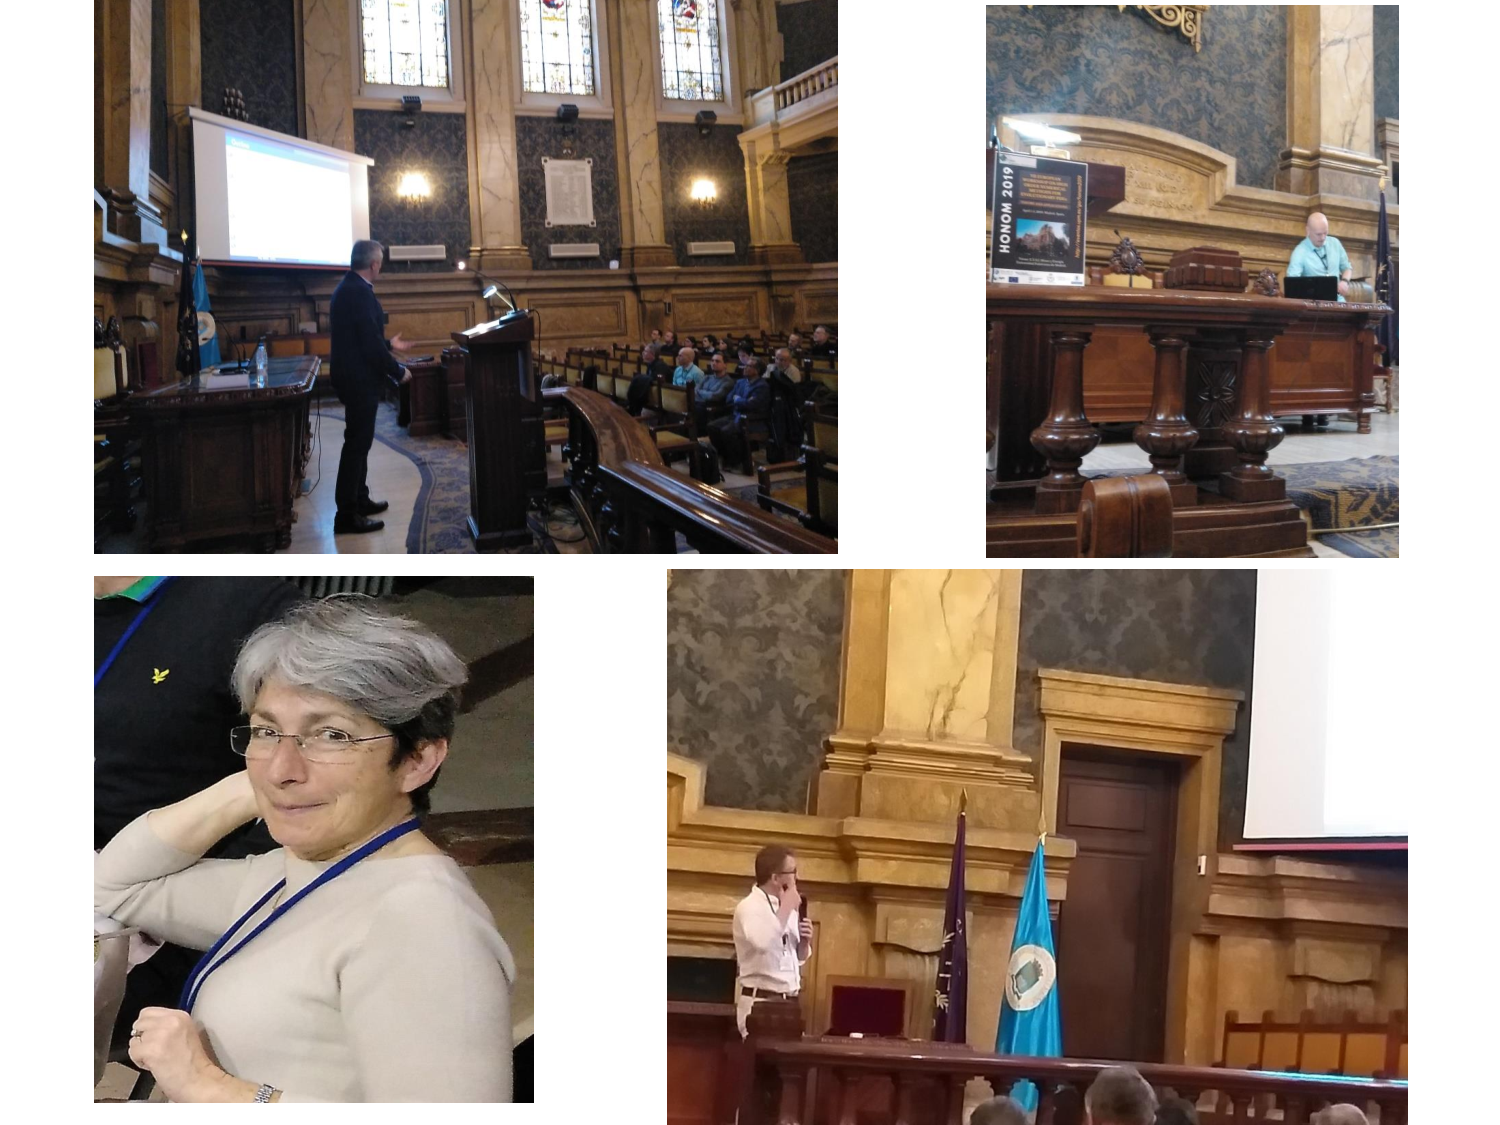
\includegraphics[width=1.2\textwidth]{FotosInv1}
	\label{fig:Invitados1}
	\caption{Conferenciantes invitados. Foto superior (izquierda a derecha): Pep Mulet e Ilya Peshkov. Foto inferior (de izquierda a derecha): Gabriella Puppo y Raphaël Loubère  - Fuente: Comité Organizador}
\end{figure}
\end{center}
%
\begin{center}
\begin{figure}
	\centering
		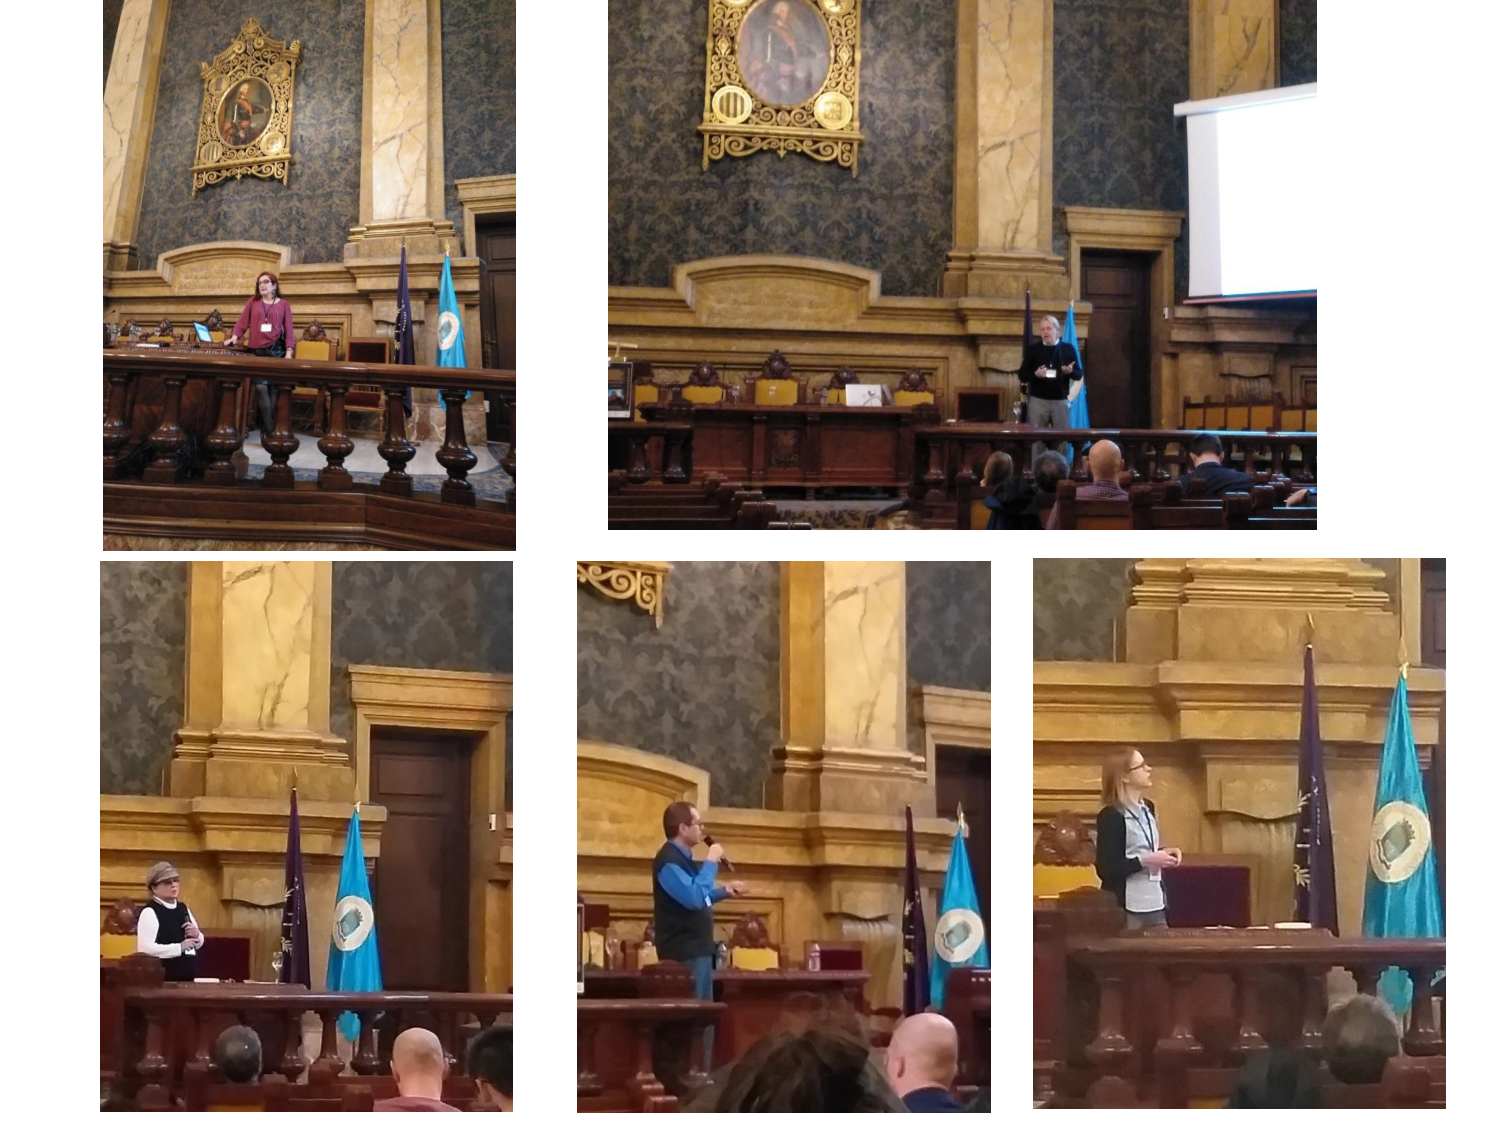
\includegraphics[width=1.2\textwidth]{FotosInv2}
	\label{fig:Invitados2}
	\caption{Foto superior (izquierda a derecha): Mª Elena Vázquez Cendón y Jan Hesthaven. Foto inferior (de izquierda a derecha): Helen Yee, Vladimir Titarev y Svetlana Tokareva  - Fuente: Comité Organizador}
\end{figure}
\end{center}

\subsection{Contribuciones y sesiones paralelas}

%
%Entre las $53$ comunicaciones orales que se presentaron se pueden destacar la de Manuel J. Castro, Carlos Parés, David Kopriva, Eleuterio F. Toro, Michael Dumbser, Jan Nordström, Gregor Gassner, Florian Hindenlang, Toni Baeza, Walter Boscheri, Tan Bui, entre muchos otros. La mayor parte de estas contribuciones se desarrollaron en dos sesiones paralelas cada día.

Tanto en las sesiones plenarias como en las comunicaciones orales se trataron diversos temas relacionados con la resolución numérica de problemas representados por leyes de conservación hiperbólicas como leyes de balance (es decir, leyes de conservación con términos fuente). La mayor parte de los trabajos presentados se basaron en esquemas numéricos de volúmenes finitos y de Galerkin discontinuo, si bien hubo también bastantes aportaciones en el contexto de métodos de elementos finitos, como en la comunicación de P. Bacigaluppi, en la que se presentaba una variante de dicho método empleando esquemas de distribución residual de alto orden. Otras comunicaciones se basaban también en métodos de elementos finitos como fue el caso, por ejemplo, de las de M. Bragin o P. Öffner. Con el fin de conseguir esquemas de orden alto en tiempo, gran parte de los trabajos utilizaban métodos IMEX (\textbf{Im}plícitos-\textbf{Ex}plícitos) tipo Runge-Kutta empleando la parte explícita para los términos hiperbólicos y la parte implícita para el tratamiento de términos fuente rígidos, como en la comunicación de G. Bertaglia, o de los términos difusivos, como en la conferencia plenaria de P. Mulet. En otras aplicaciones se emplearon esquemas numéricos tipo ADER con el fin de conseguir orden arbitrario en tiempo. En este sentido, es interesante destacar que estos métodos fueron introducidos por E.F. Toro, quien forma parte del Comité Organizador de HONOM y participó como ponente en la presente edición, junto con V. Titarev que fue conferenciante plenario de este congreso. Una reciente versión de los esquemas ADER, denominada \textit{Local-Space Time Discontinuous Galerkin} (LSTDG) fue introducida por M. Dumbser, quien forma, asimismo, parte del Comité Organizador de HONOM y también presentó una comunicación en este Congreso. Mediante estos esquemas tipo ADER se consigue un orden arbitrario en espacio y tiempo en un sólo paso, sin necesidad de emplear varias etapas intermedias, como sucede en los métodos de Runge-Kutta, tal como quedó patente en alguna de las comunicaciones presentadas. Algunas de las comunicaciones en las que se empleaban los esquemas ADER fueron las de M. Dumbser, E.F. Toro, M. Tavelli, F. Fambri, M. Ioratti o la plenaria de I. Peshkov. En muchos de los trabajos se emplearon esquemas numéricos tipo WENO (Weighted Essentially Non Oscillatory) y CWENO (Central WENO) para conseguir reconstrucciones espaciales de alto orden, especialmente en el contexto de los métodos en volúmenes finitos. En la comunicación de A. Baeza se presentó un cálculo eficiente de los indicadores de suavidad para los métodos WENO. Interesantes también fueron trabajos basados en técnicas numéricas de Galerkin discontinuo, las cuales, en algunos casos, se han complementado con limitadores de flujo \textit{a posteriori} basados en volúmenes finitos, en el interior de celdas \textit{conflictivas}, con el fin de conseguir esquemas más eficientes. Trabajos en esta línea fueron, por ejemplo, los de M.J. Castro, W. Boscheri, M. Tavelli, M. Ioratti o la plenaria de R. Loubère, en las que se hacía uso del paradigma MOOD. También se presentaron esquemas en Galerkin discontinuo semimplícitos de alto orden, sobre mallados \textit{staggered} no estructurados, como en la comunicación presentada por S. Busto. Hubo algunas comunicaciones, como las de F. Fambri, M. Tavelli y G. Gassner, en las que se empleaban esquemas numéricos basados en refinamiento adaptativo del mallado (AMR por sus siglas en inglés) que mejoran sustancialmente el tiempo de cálculo refinando sólo donde es necesario y desrefinando cuando deja de serlo. Otros problemas que en plantearon fueron en un contexto Lagrangiano-Euleriano como los denominados ALE (Arbitrary Lagrangian Eulerian), como en la comunicación de L. Saavedra. También se presentaron aplicaciones al filtrado numérico de señales, como en el caso del trabajo presentado por J. Nordström. Los modelos matemáticos tratados fueron ecuaciones de aguas someras, ecuaciones de Navier-Stokes, ecuaciones de Euler en dinámica de gases, comportamiento viscoelástico de vasos sanguíneos, ecuaciones de Cahn-Hilliard que describen la separación de fases en un fluido, ecuaciones de convección-difusión, problemas de flujo multifásico, ecuaciones de Baer-Nunziato para flujo bifásico, problemas de mecánica de sólidos, mecánica de medios continuos o problemas de electromagnetismo entre otros. Hubo además trabajos relacionados con redes neuronales, como la plenaria de J. Hesthaven.  También se presentaron comunicaciones de un enfoque más teórico, vinculadas a estudios teóricos de los métodos numéricos de interés en este congreso.
%
\begin{center}
\begin{figure}
	\centering
		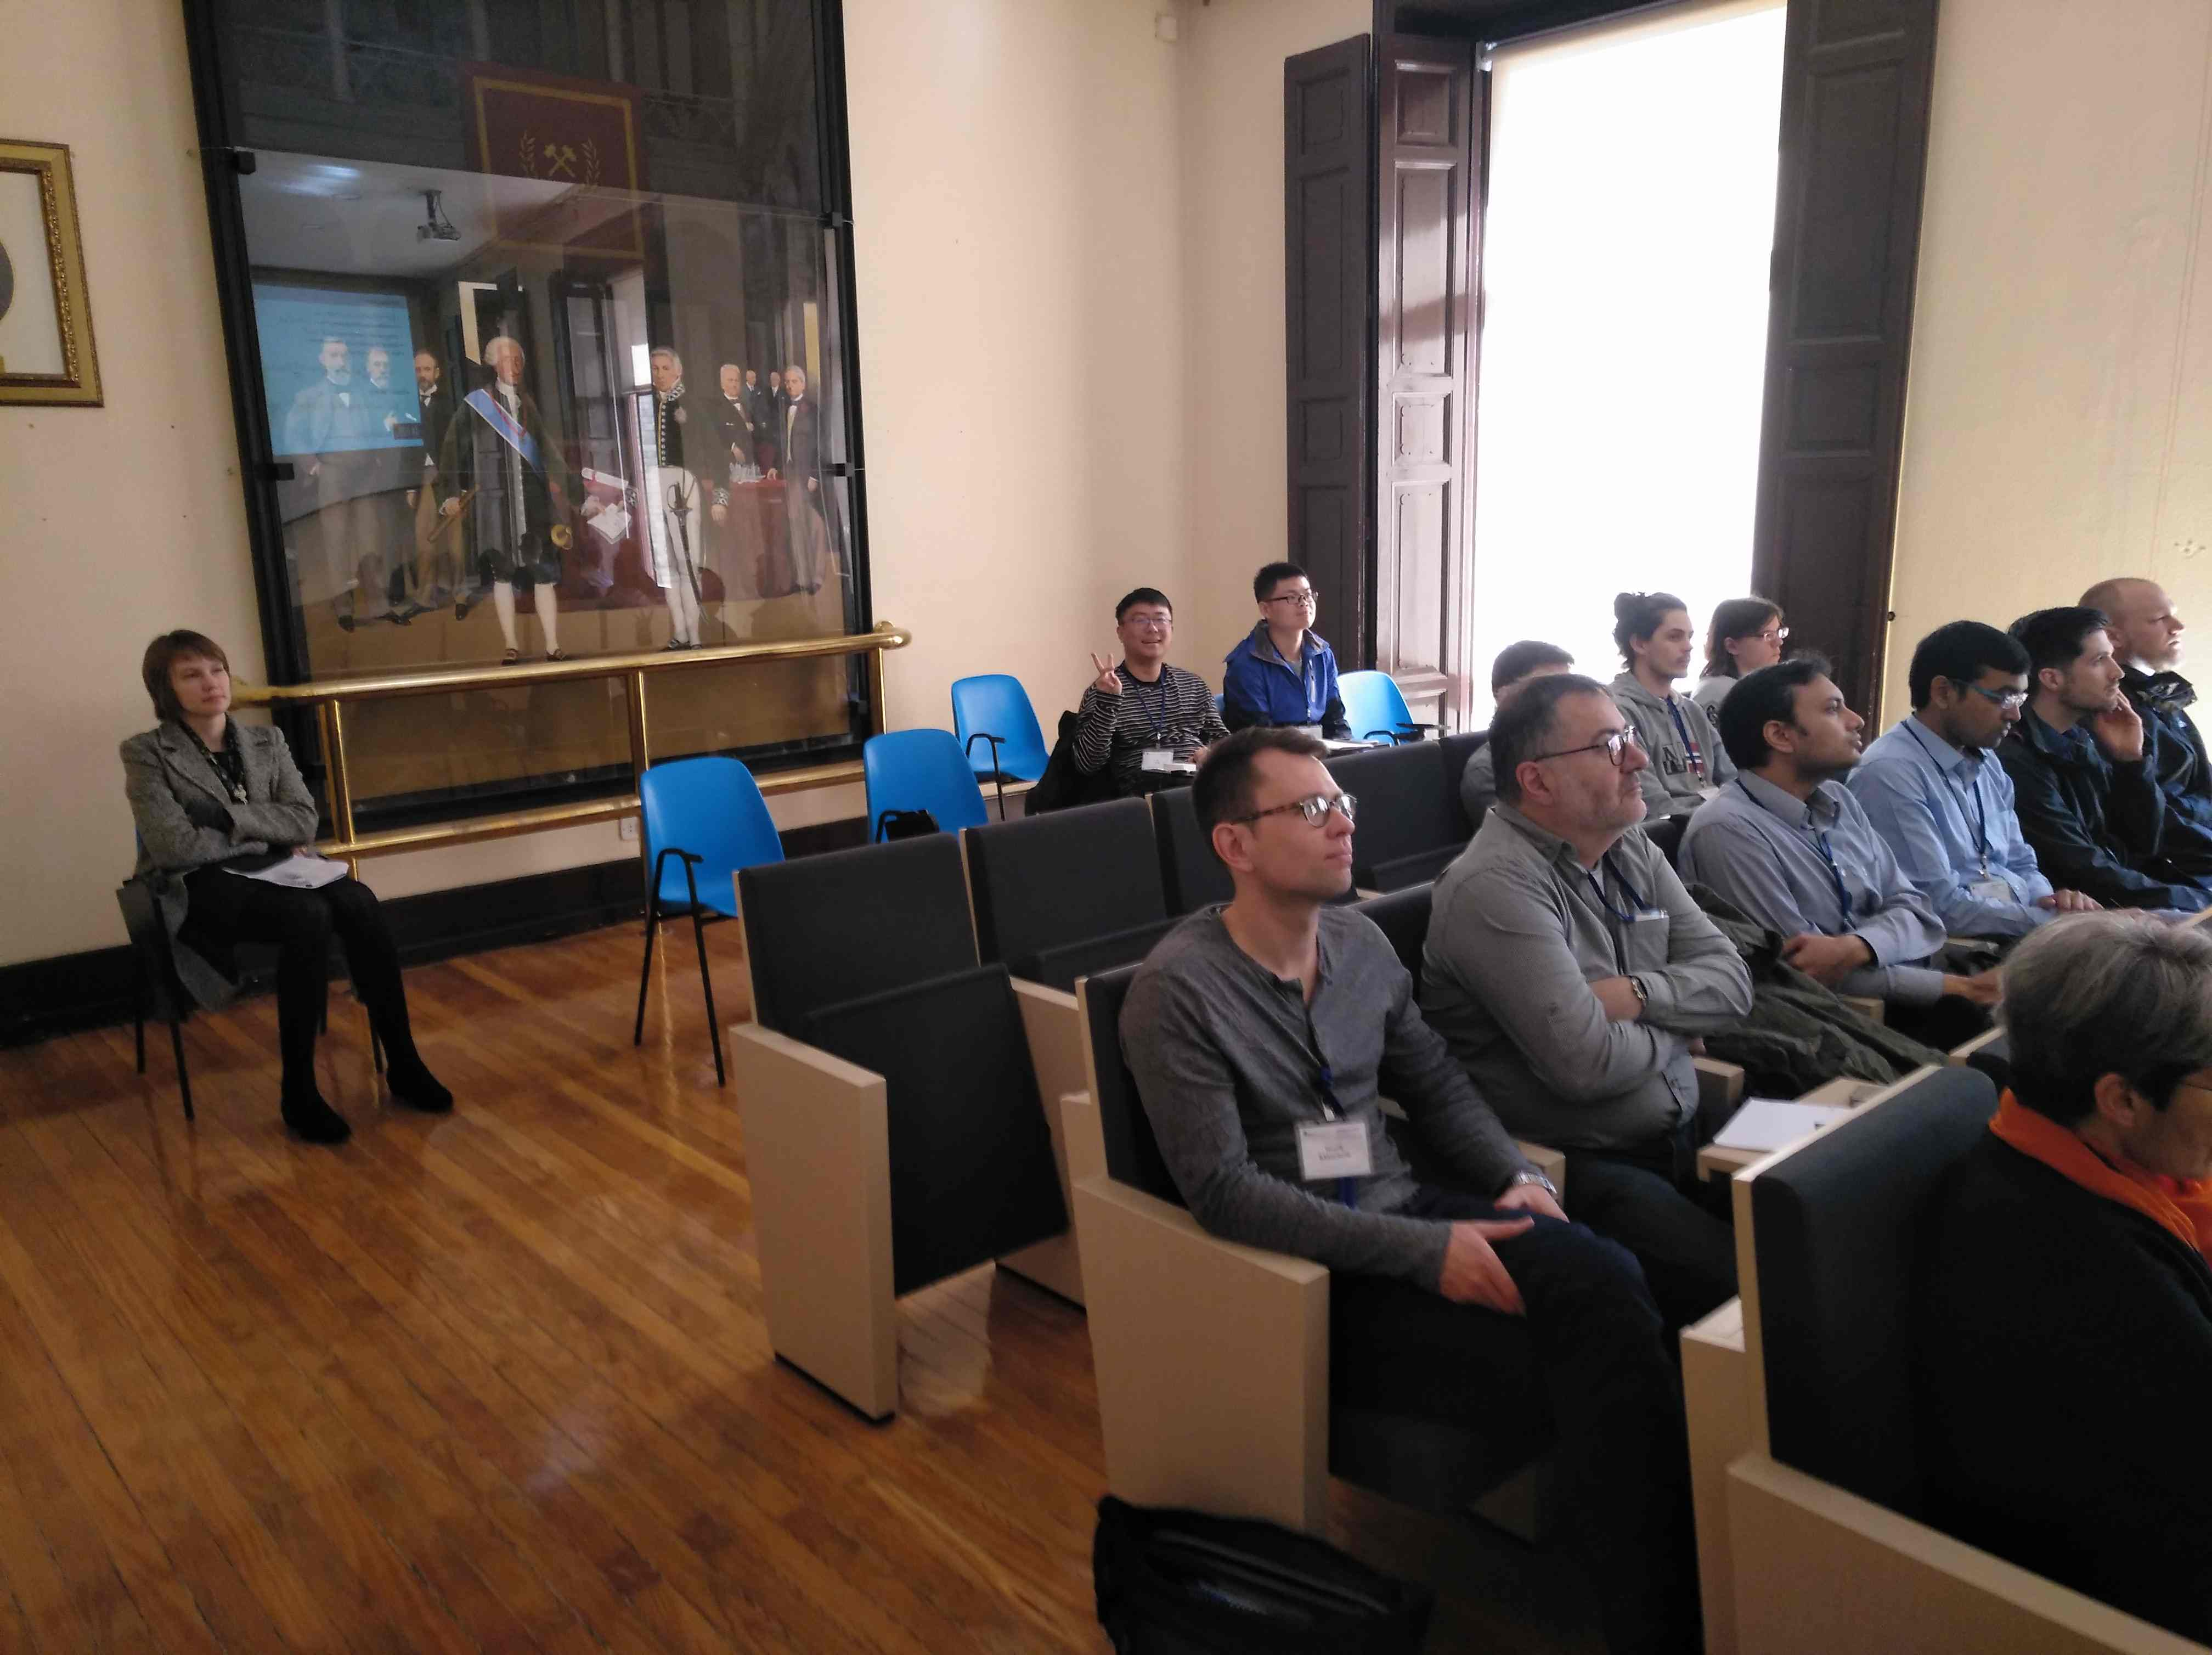
\includegraphics[width=0.7\textwidth]{Fausto}
		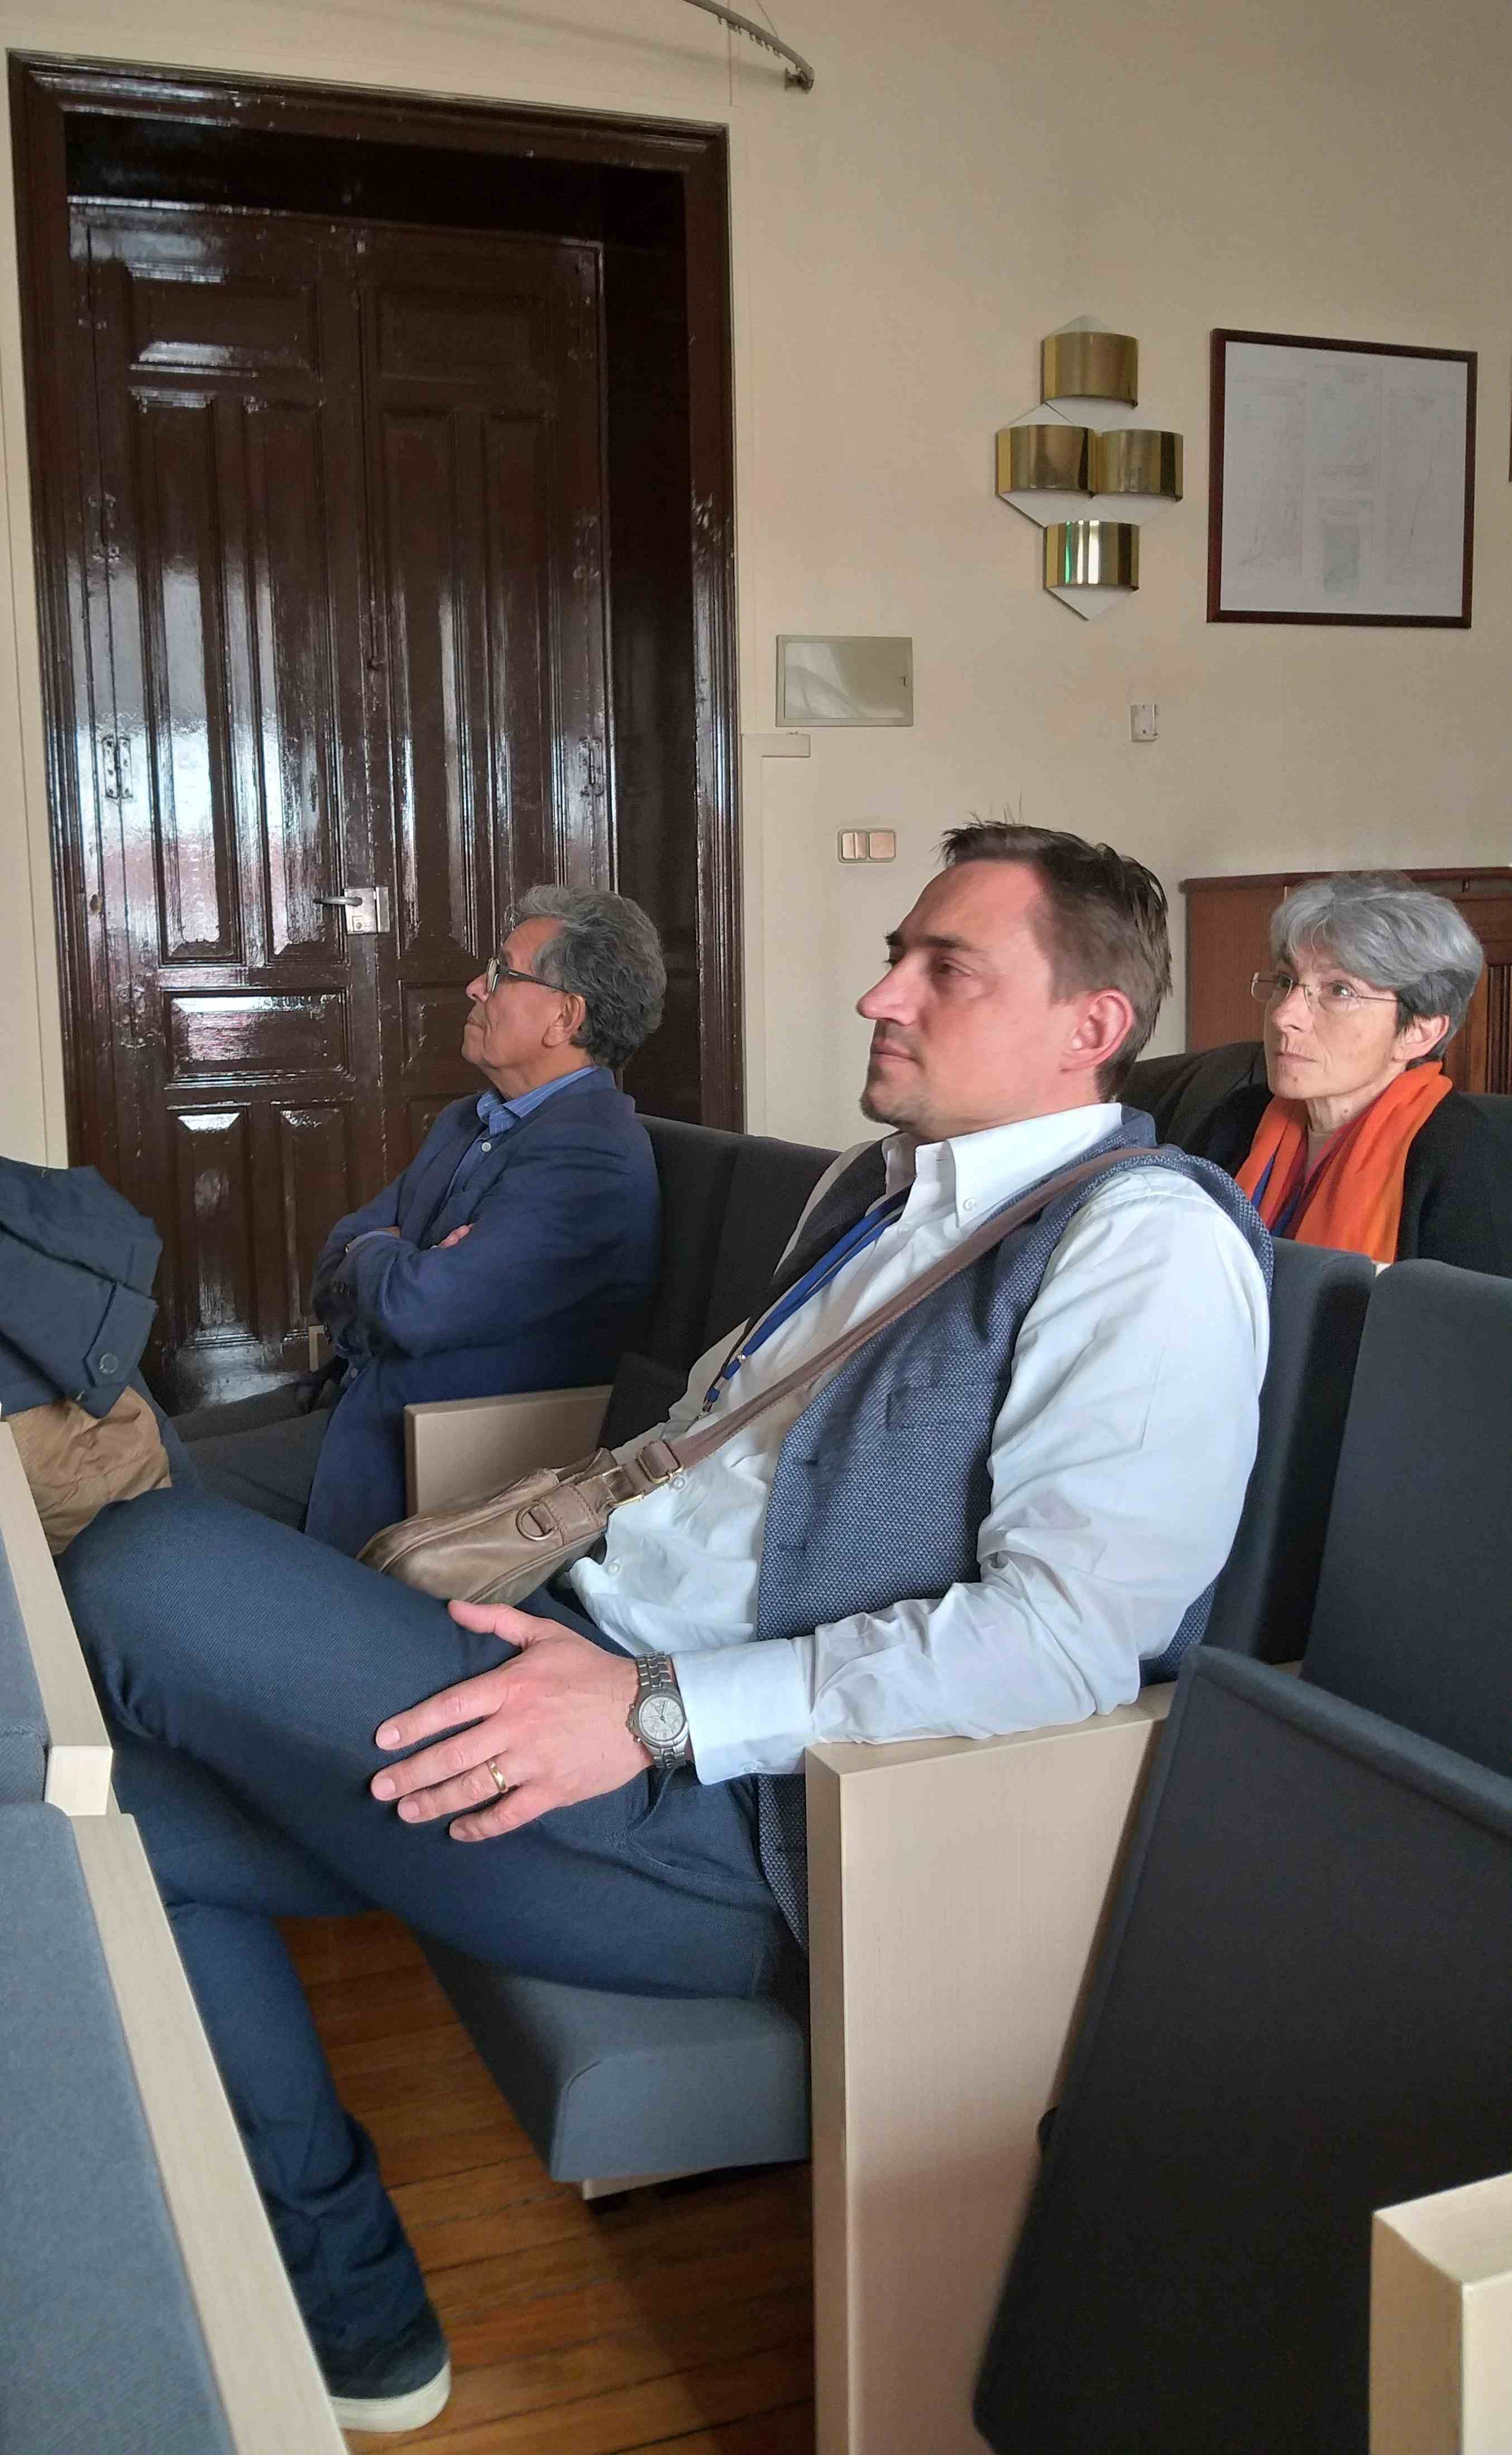
\includegraphics[width=0.7\textwidth]{Puppo-Dumbser-Toro}
	\label{fig:FaustoElh}
	\caption{Asistentes a una de las sesiones paralelas en la Sala Fausto Elhuyar de la Escuela  - Fuente: Comité Organizador}
\end{figure}
\end{center}
%
%
\begin{center}
\begin{figure}
	\centering
		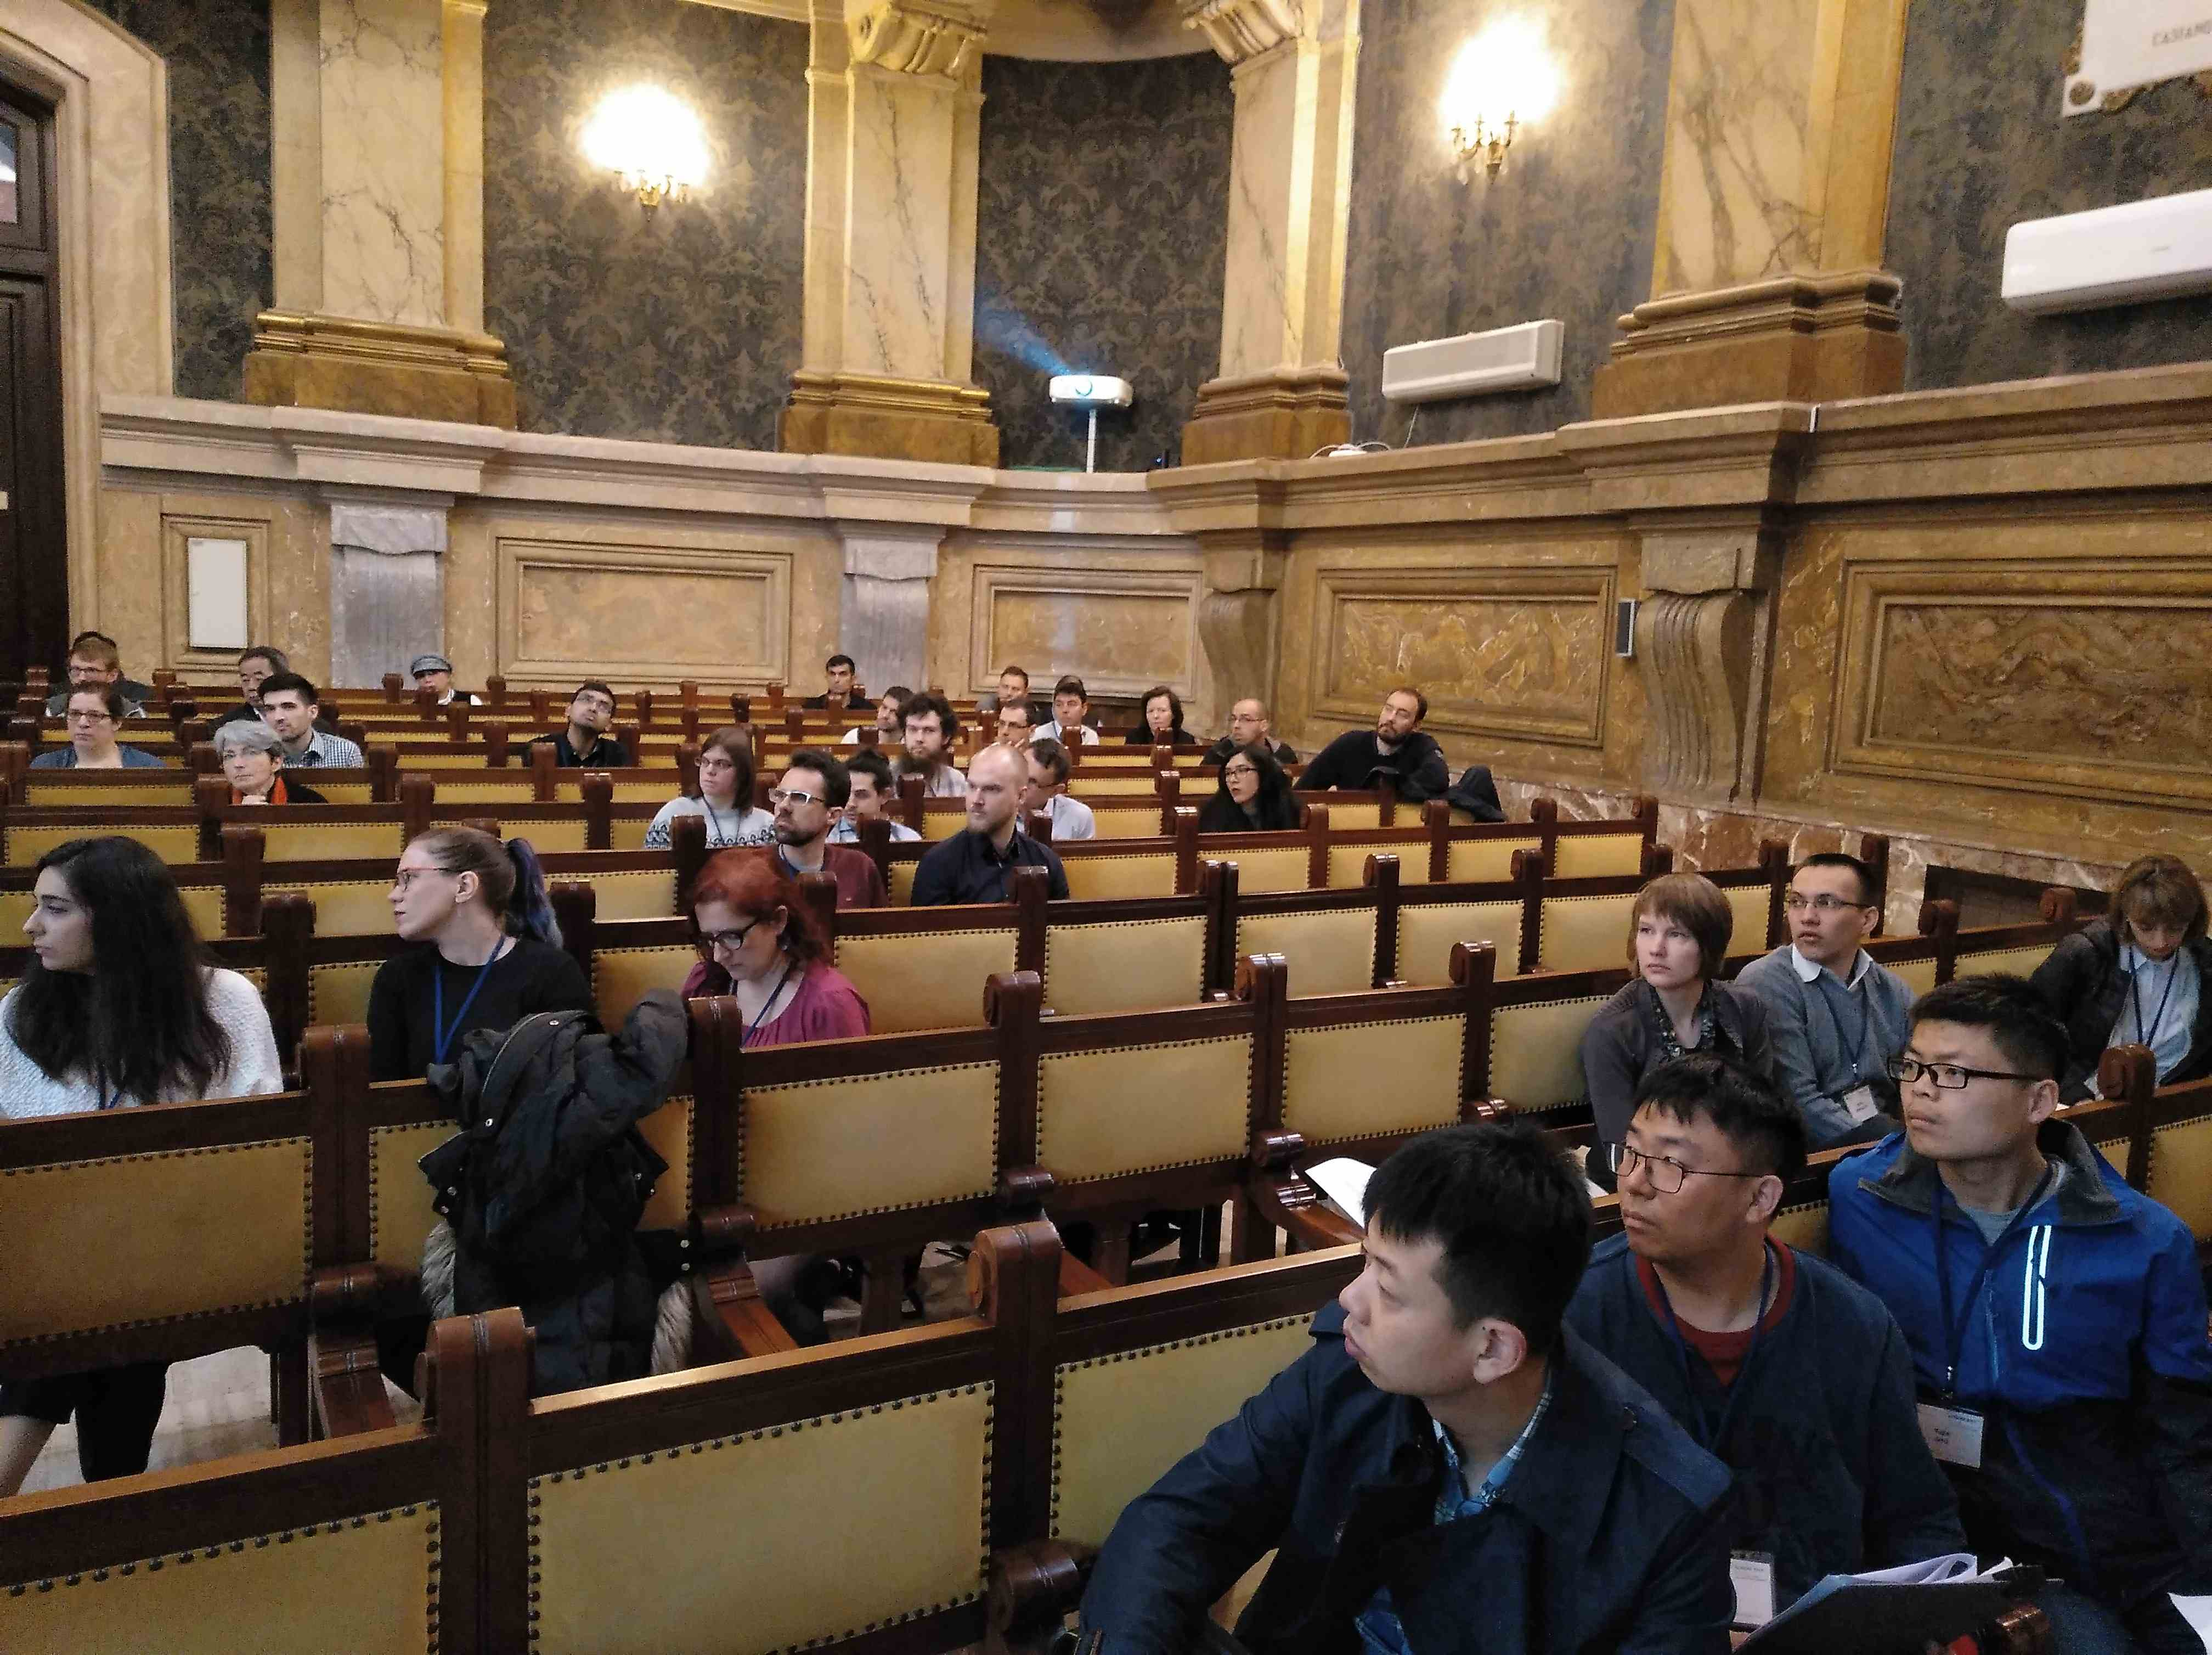
\includegraphics[width=0.9\textwidth]{SalonActos}
		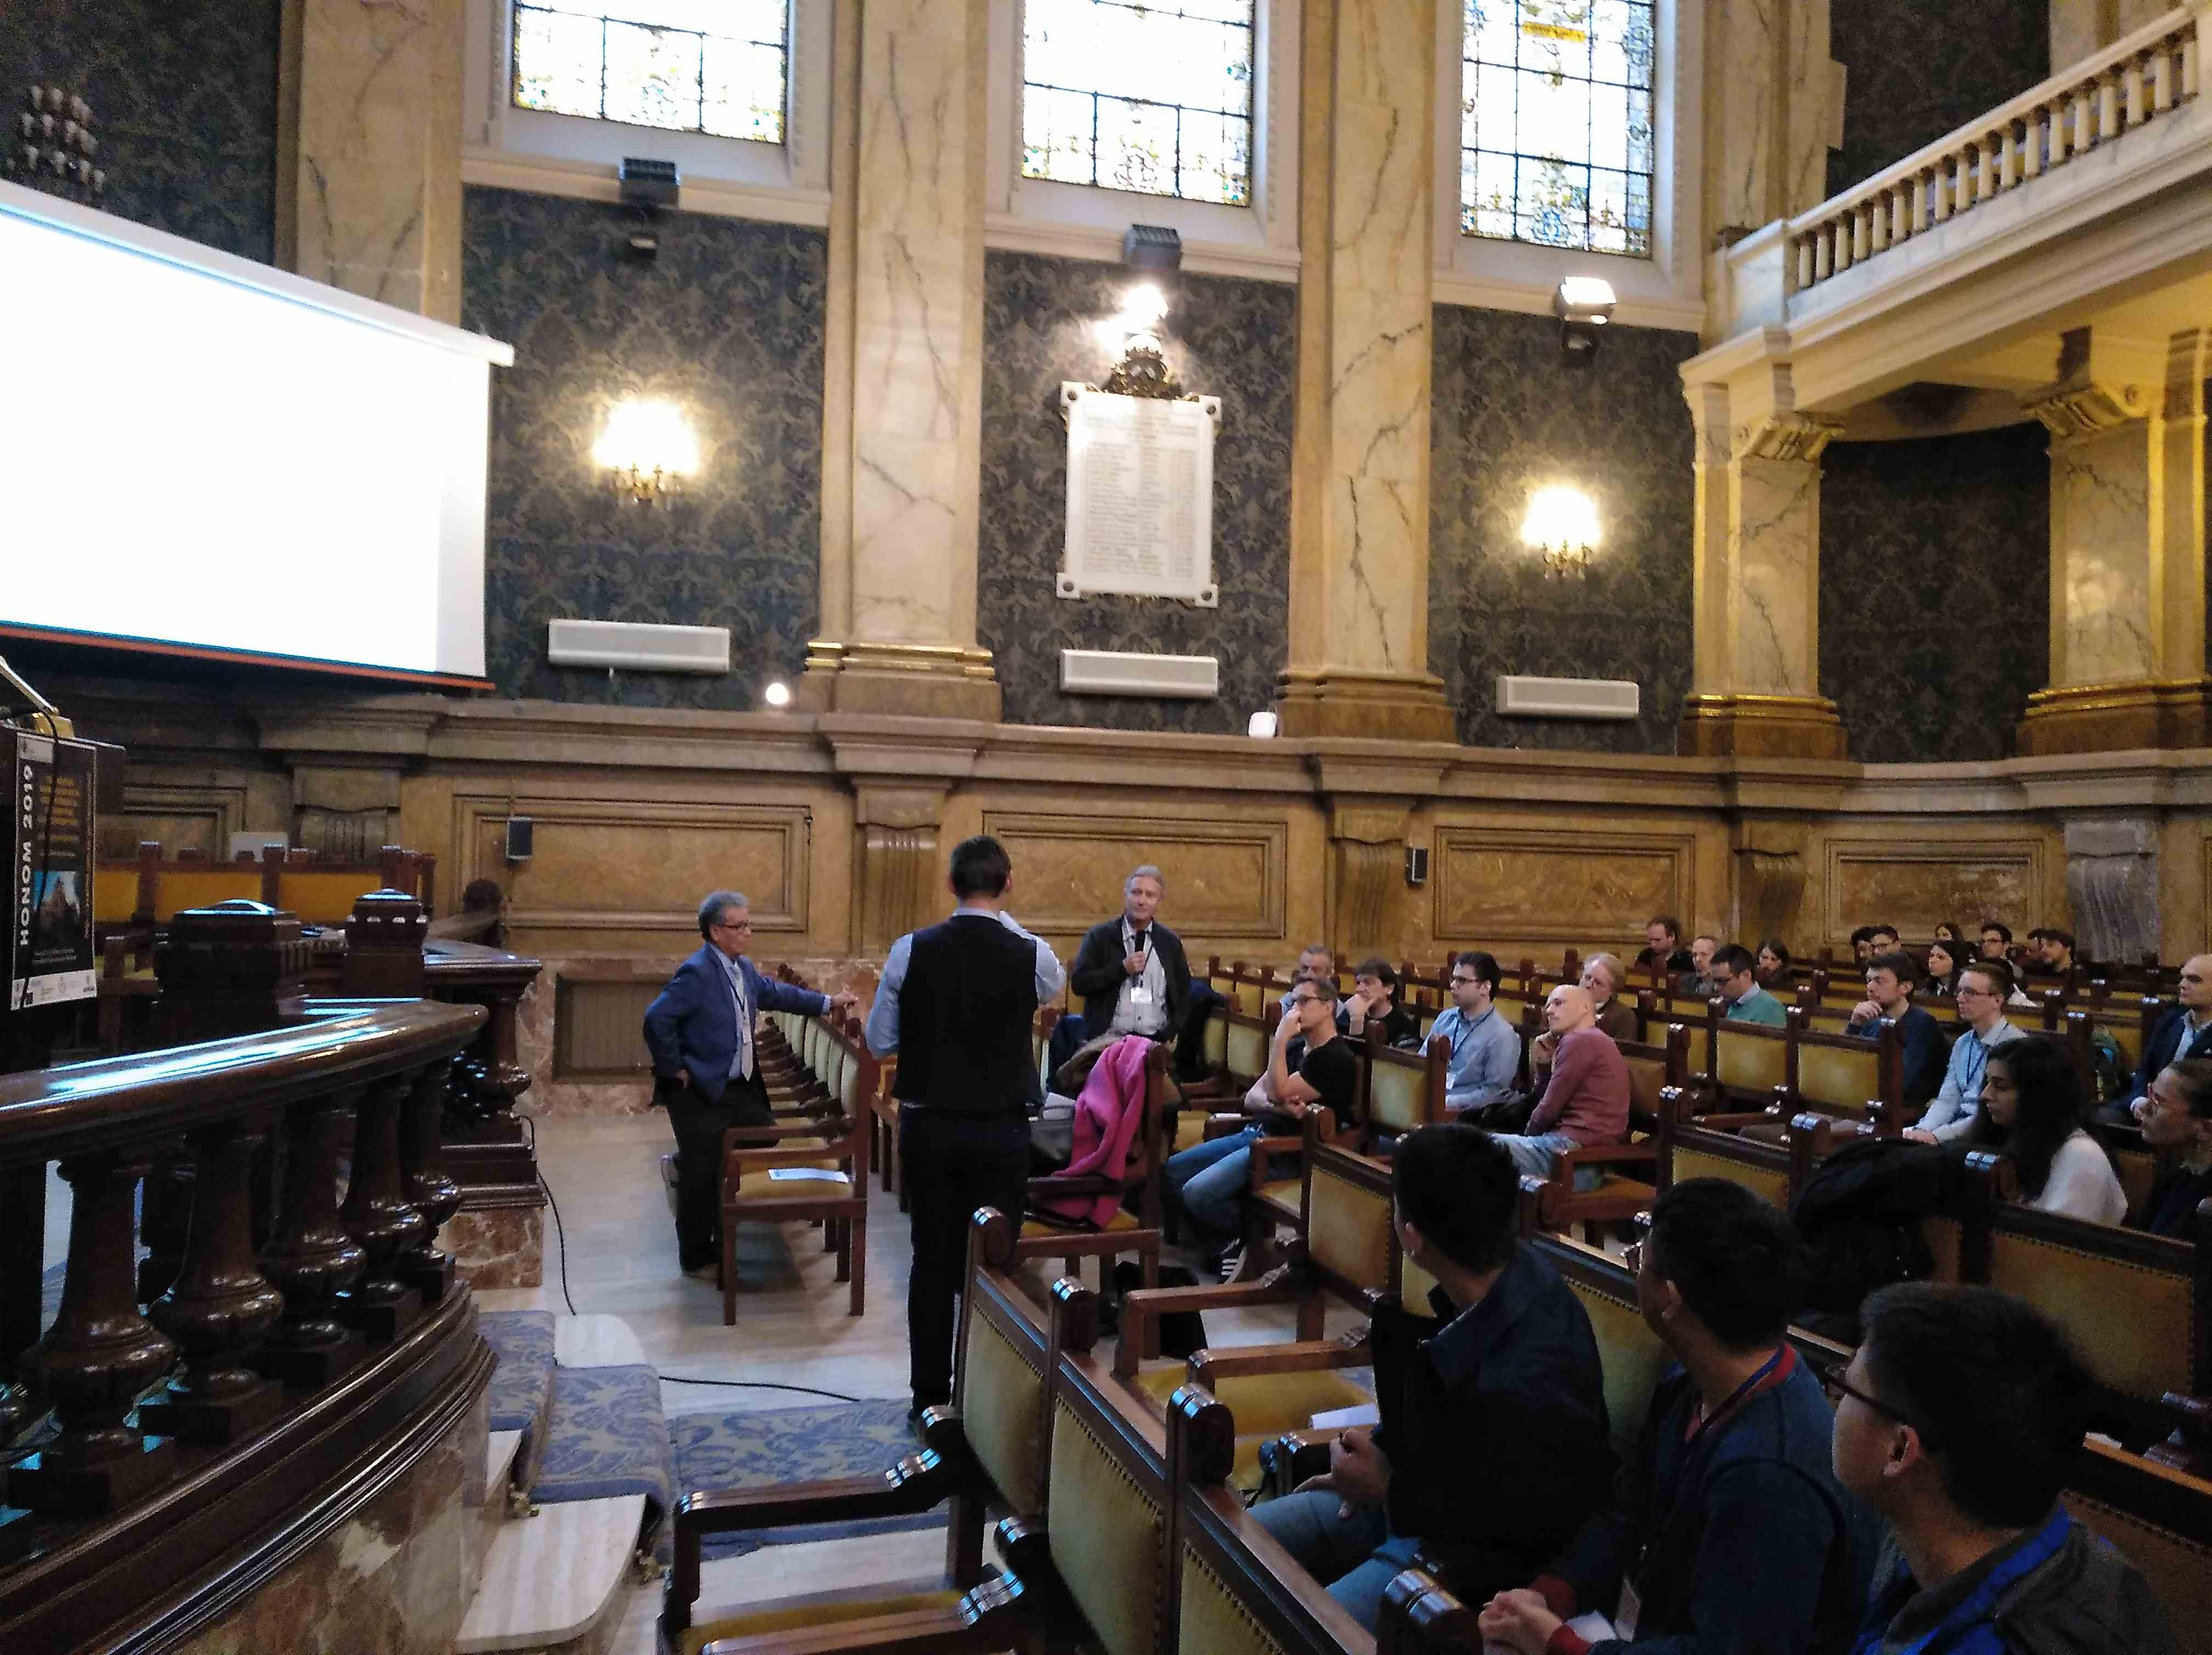
\includegraphics[width=0.9\textwidth]{SalonActos2}
	\label{fig:SalActs}
	\caption{Asistentes a una de las sesiones el Salón de Actos de la Escuela  - Fuente: Comité Organizador}
\end{figure}
\end{center}
%
\begin{center}
\begin{figure}
	\centering
		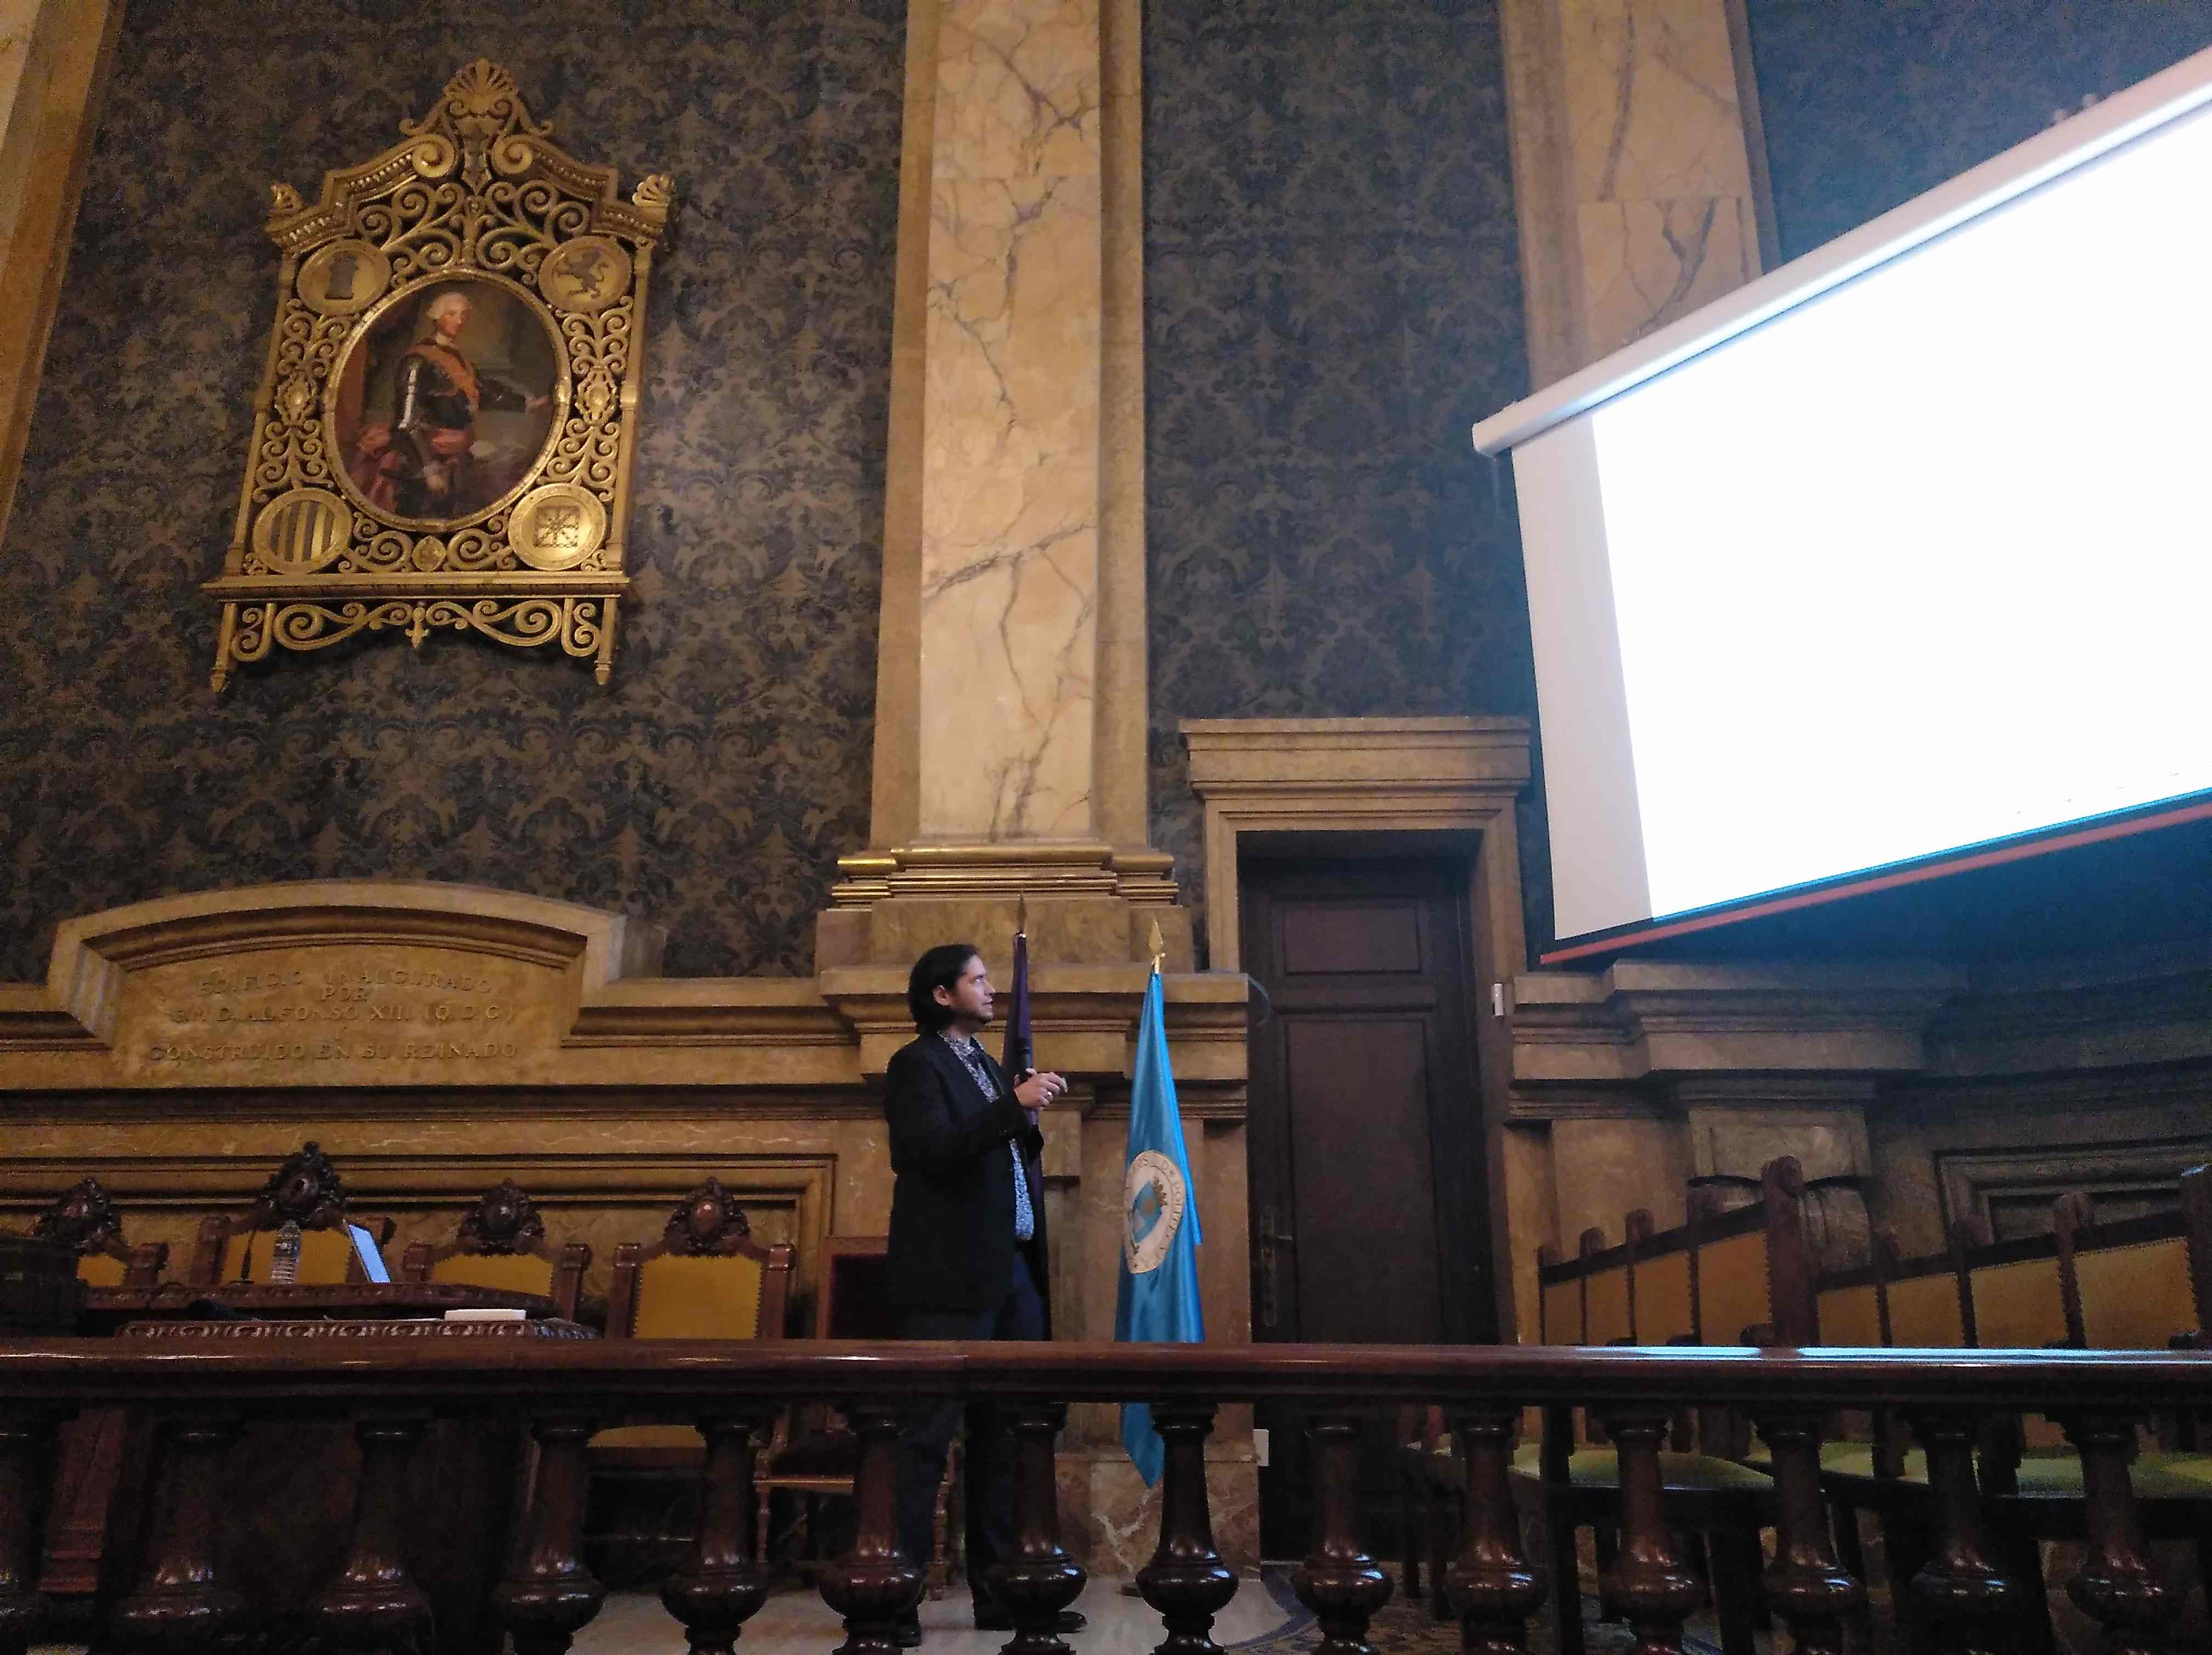
\includegraphics[width=0.9\textwidth]{GGassner}
		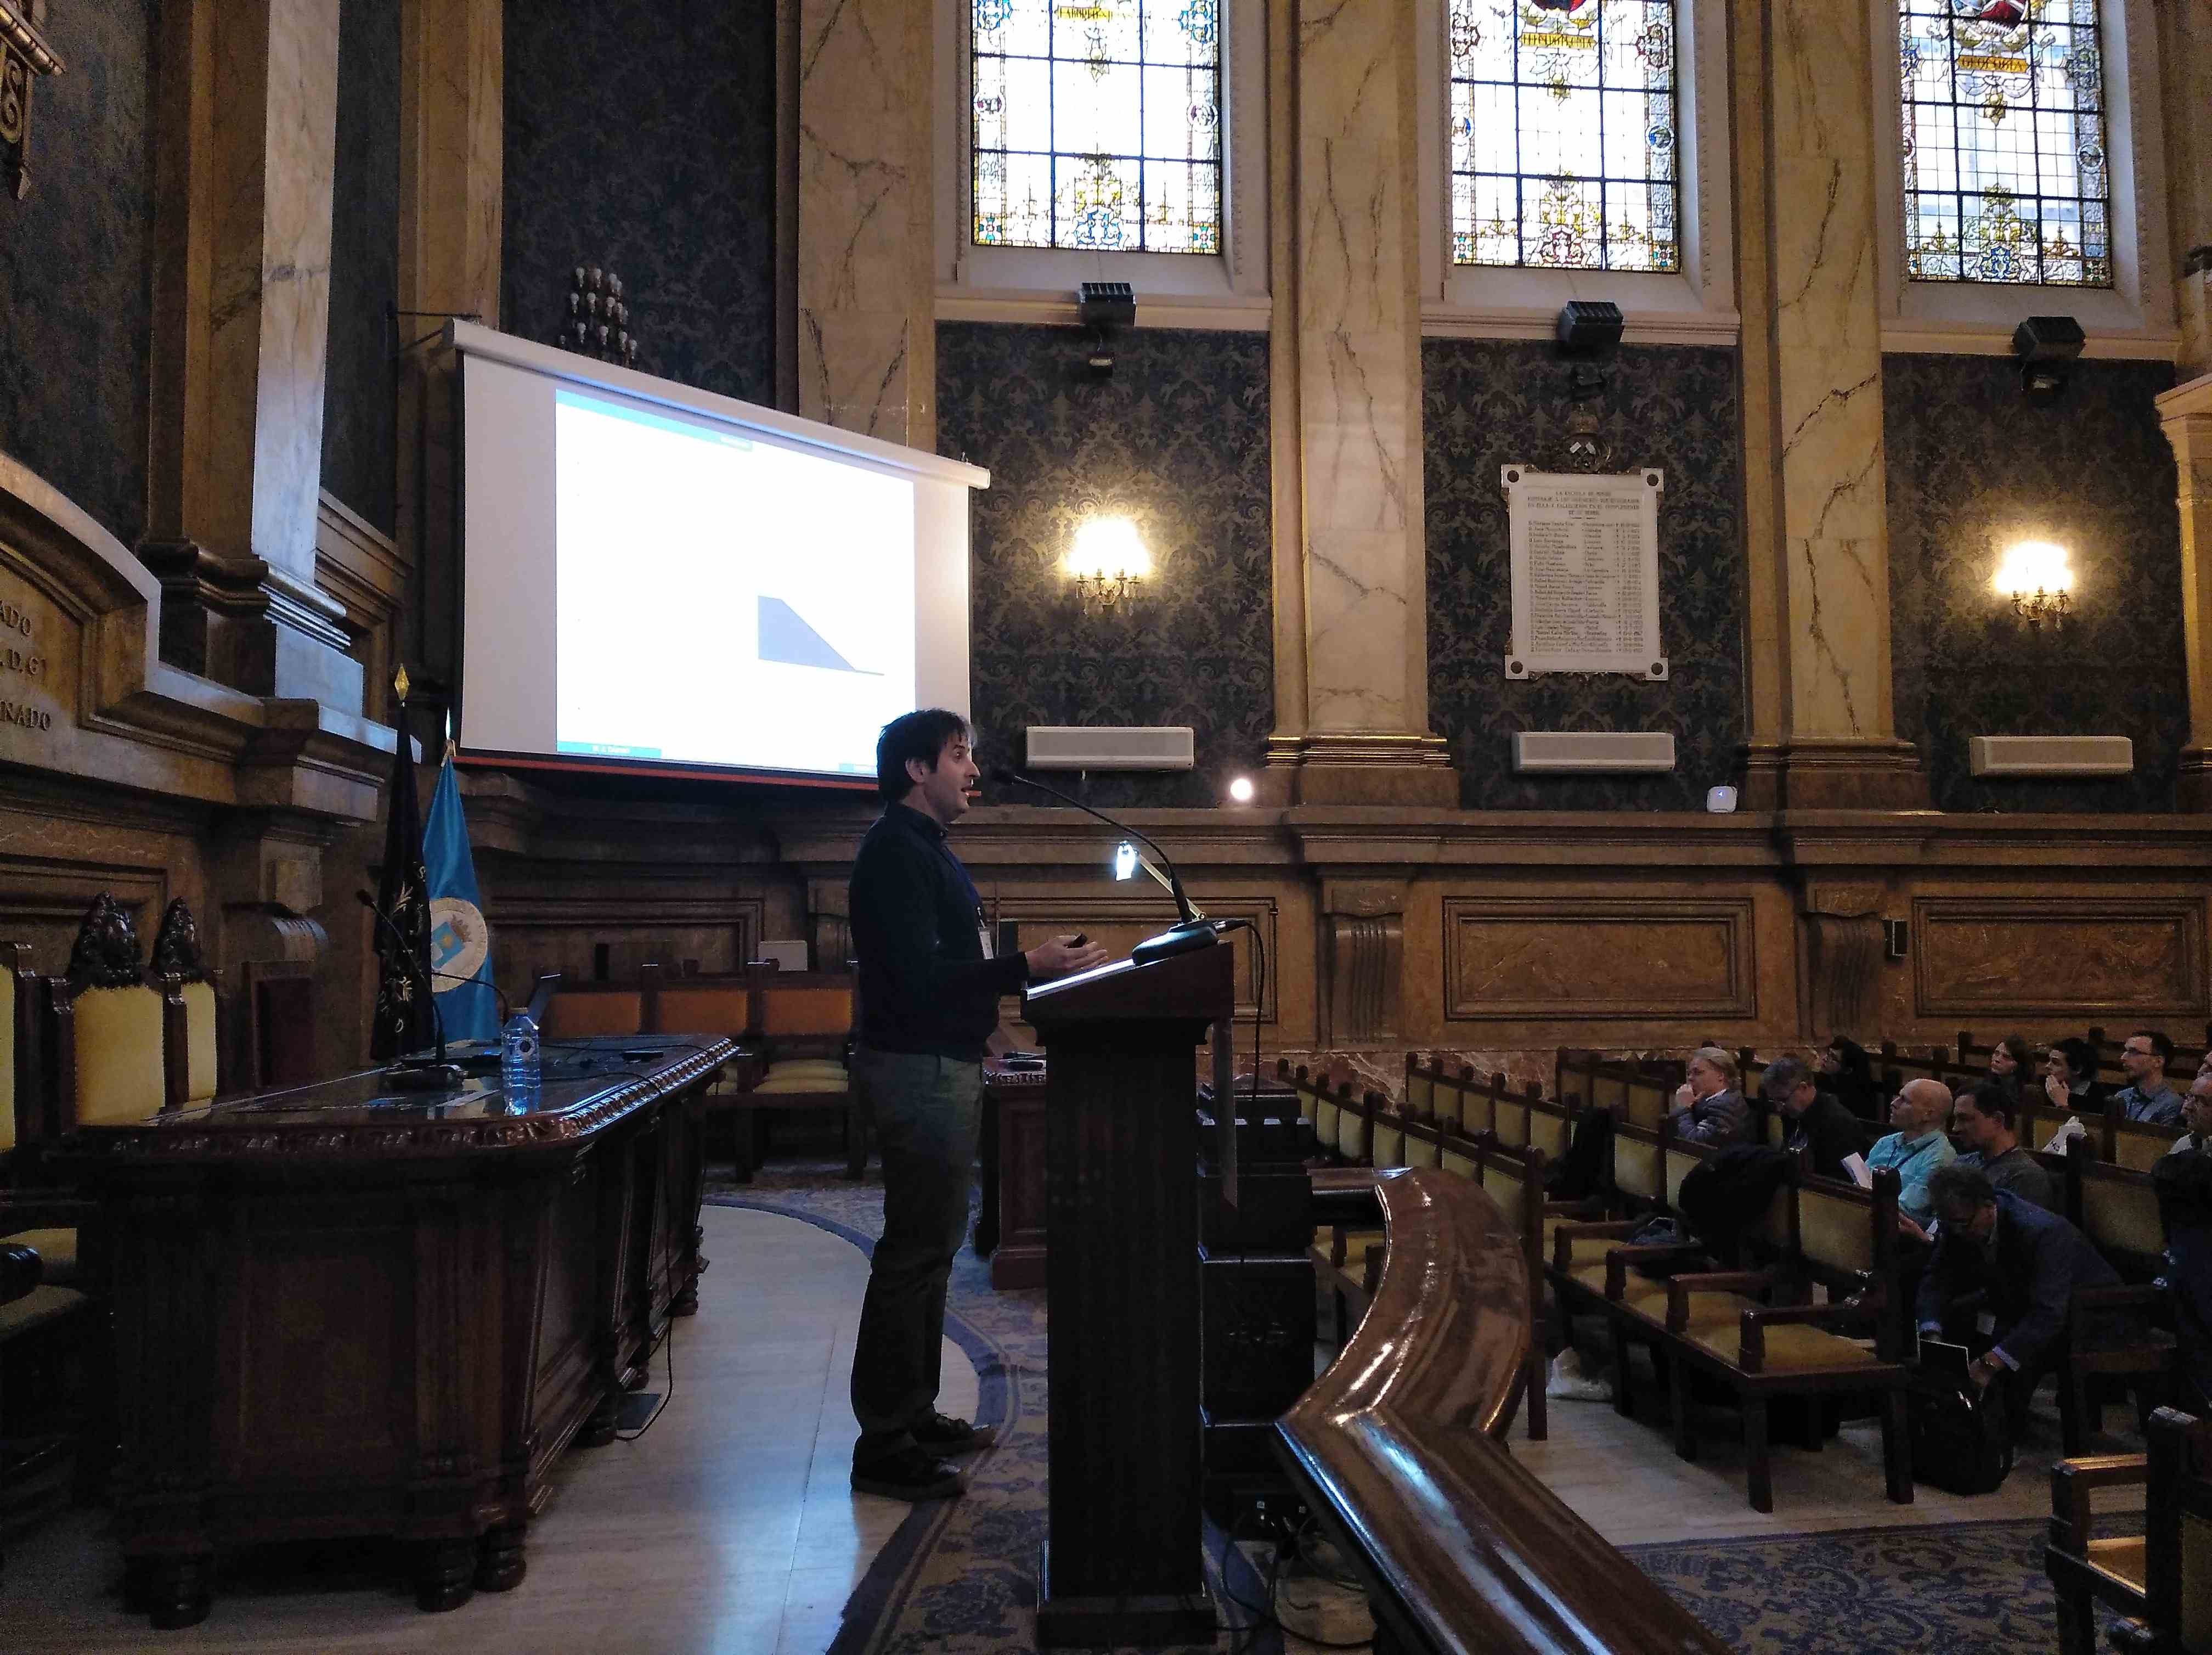
\includegraphics[width=0.9\textwidth]{MCastro}
	\label{fig:Salon1}
	\caption{Imágenes de las charlas de Gregor Gassner y Manuel J. Castro en el Salón de Actos de la ETSIME  - Fuente: Comité Organizador}
\end{figure}
\end{center}
%
\begin{center}
\begin{figure}
	\centering
		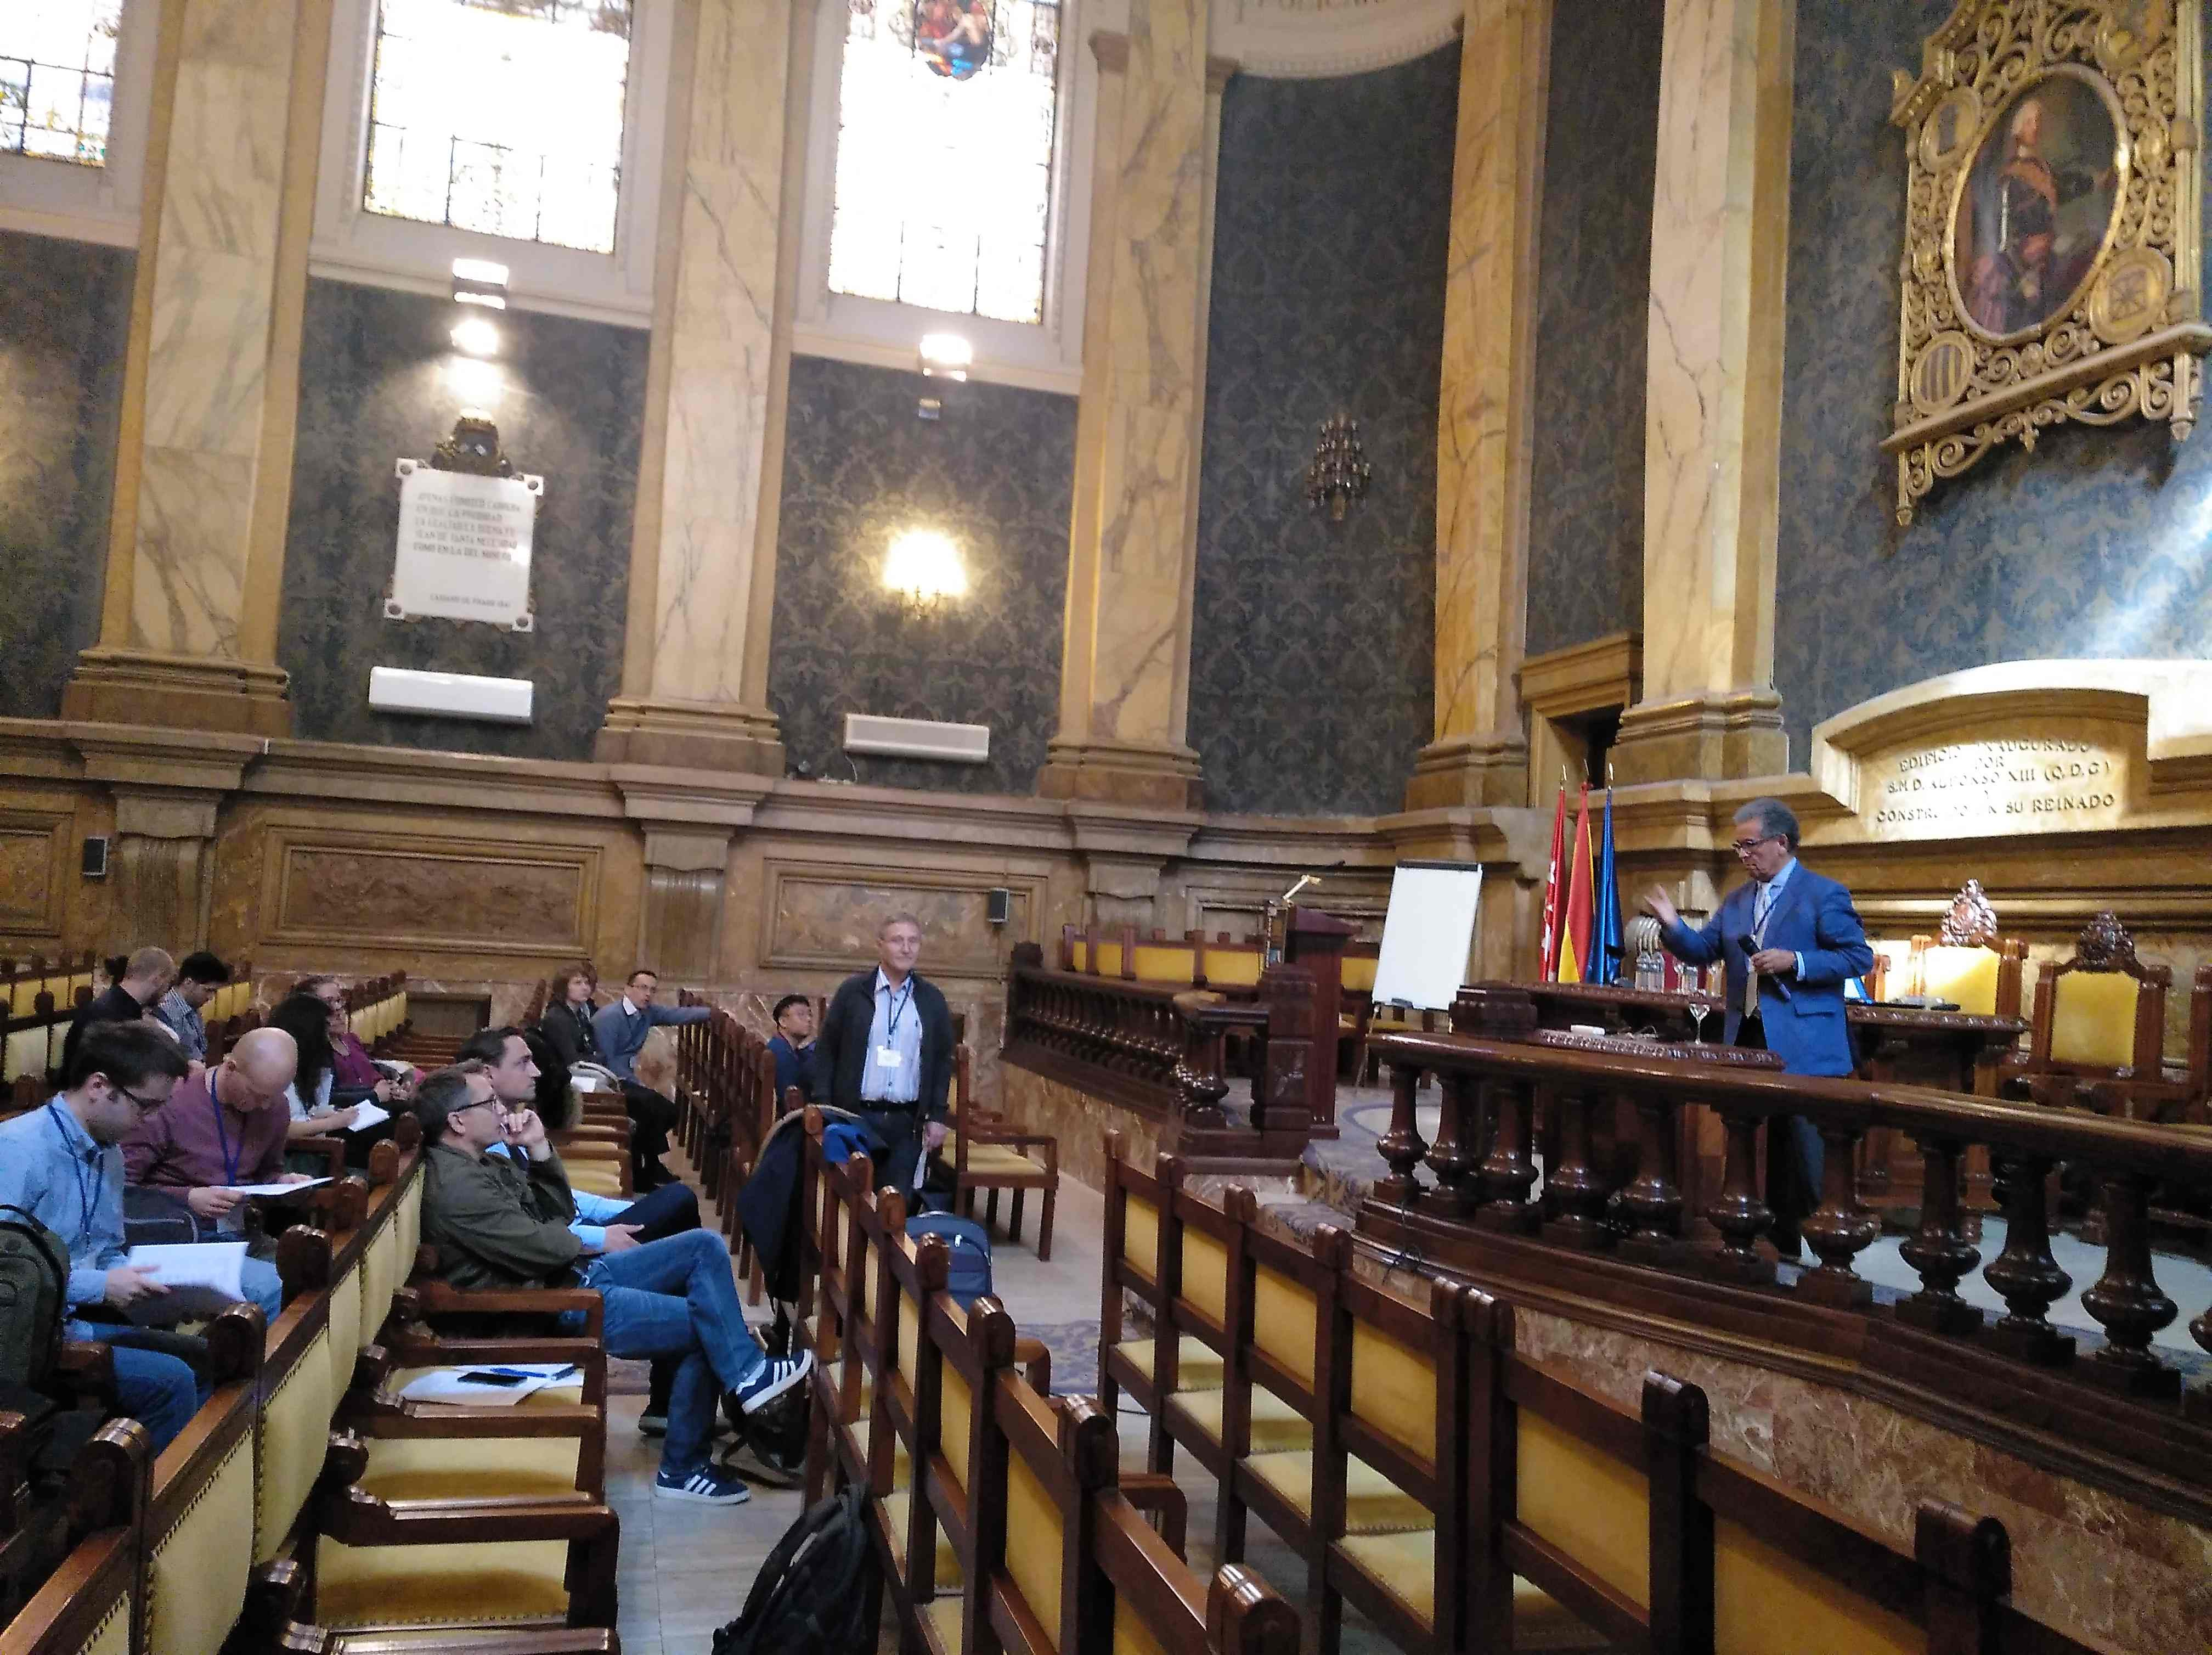
\includegraphics[width=0.9\textwidth]{EFToro}
		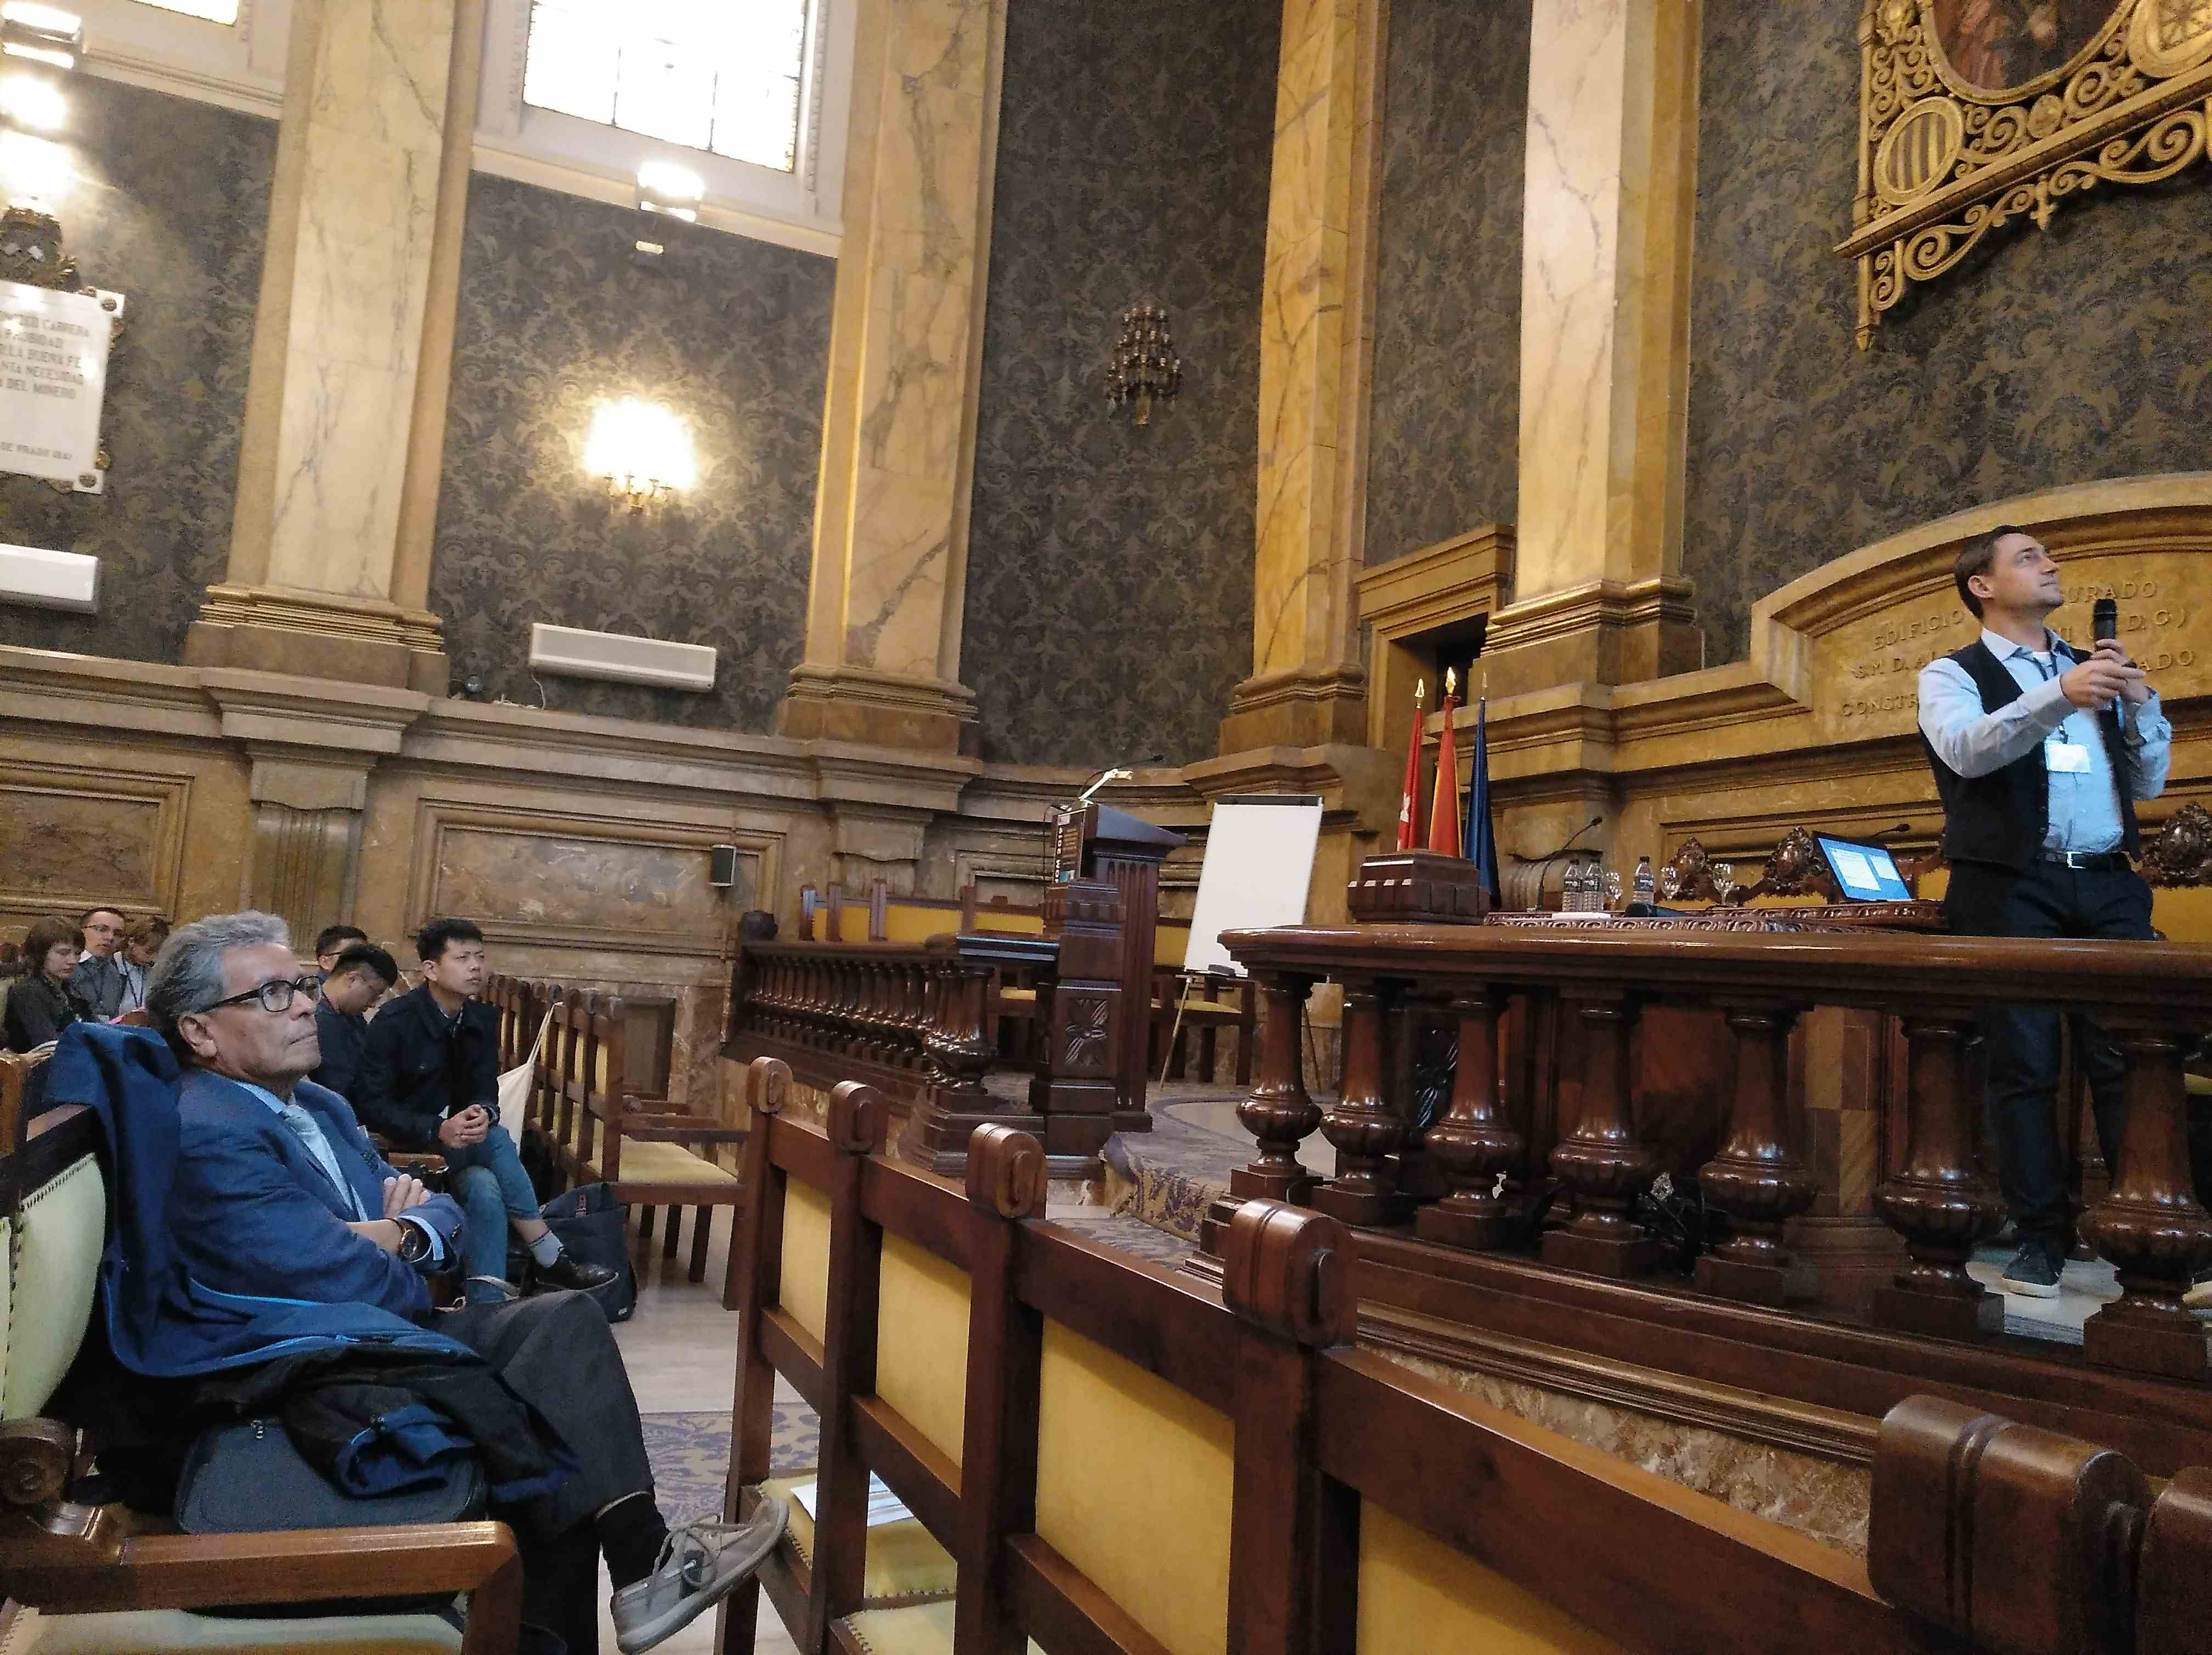
\includegraphics[width=0.9\textwidth]{MDumbser}
	\label{fig:Salon2}
	\caption{Imágenes de las charlas de Eleuterio F. Toro y Michael Dumbser en el Salón de Actos de la ETSIME  - Fuente: Comité Organizador}
\end{figure}
\end{center}
%
\begin{center}
\begin{figure}
	\centering
		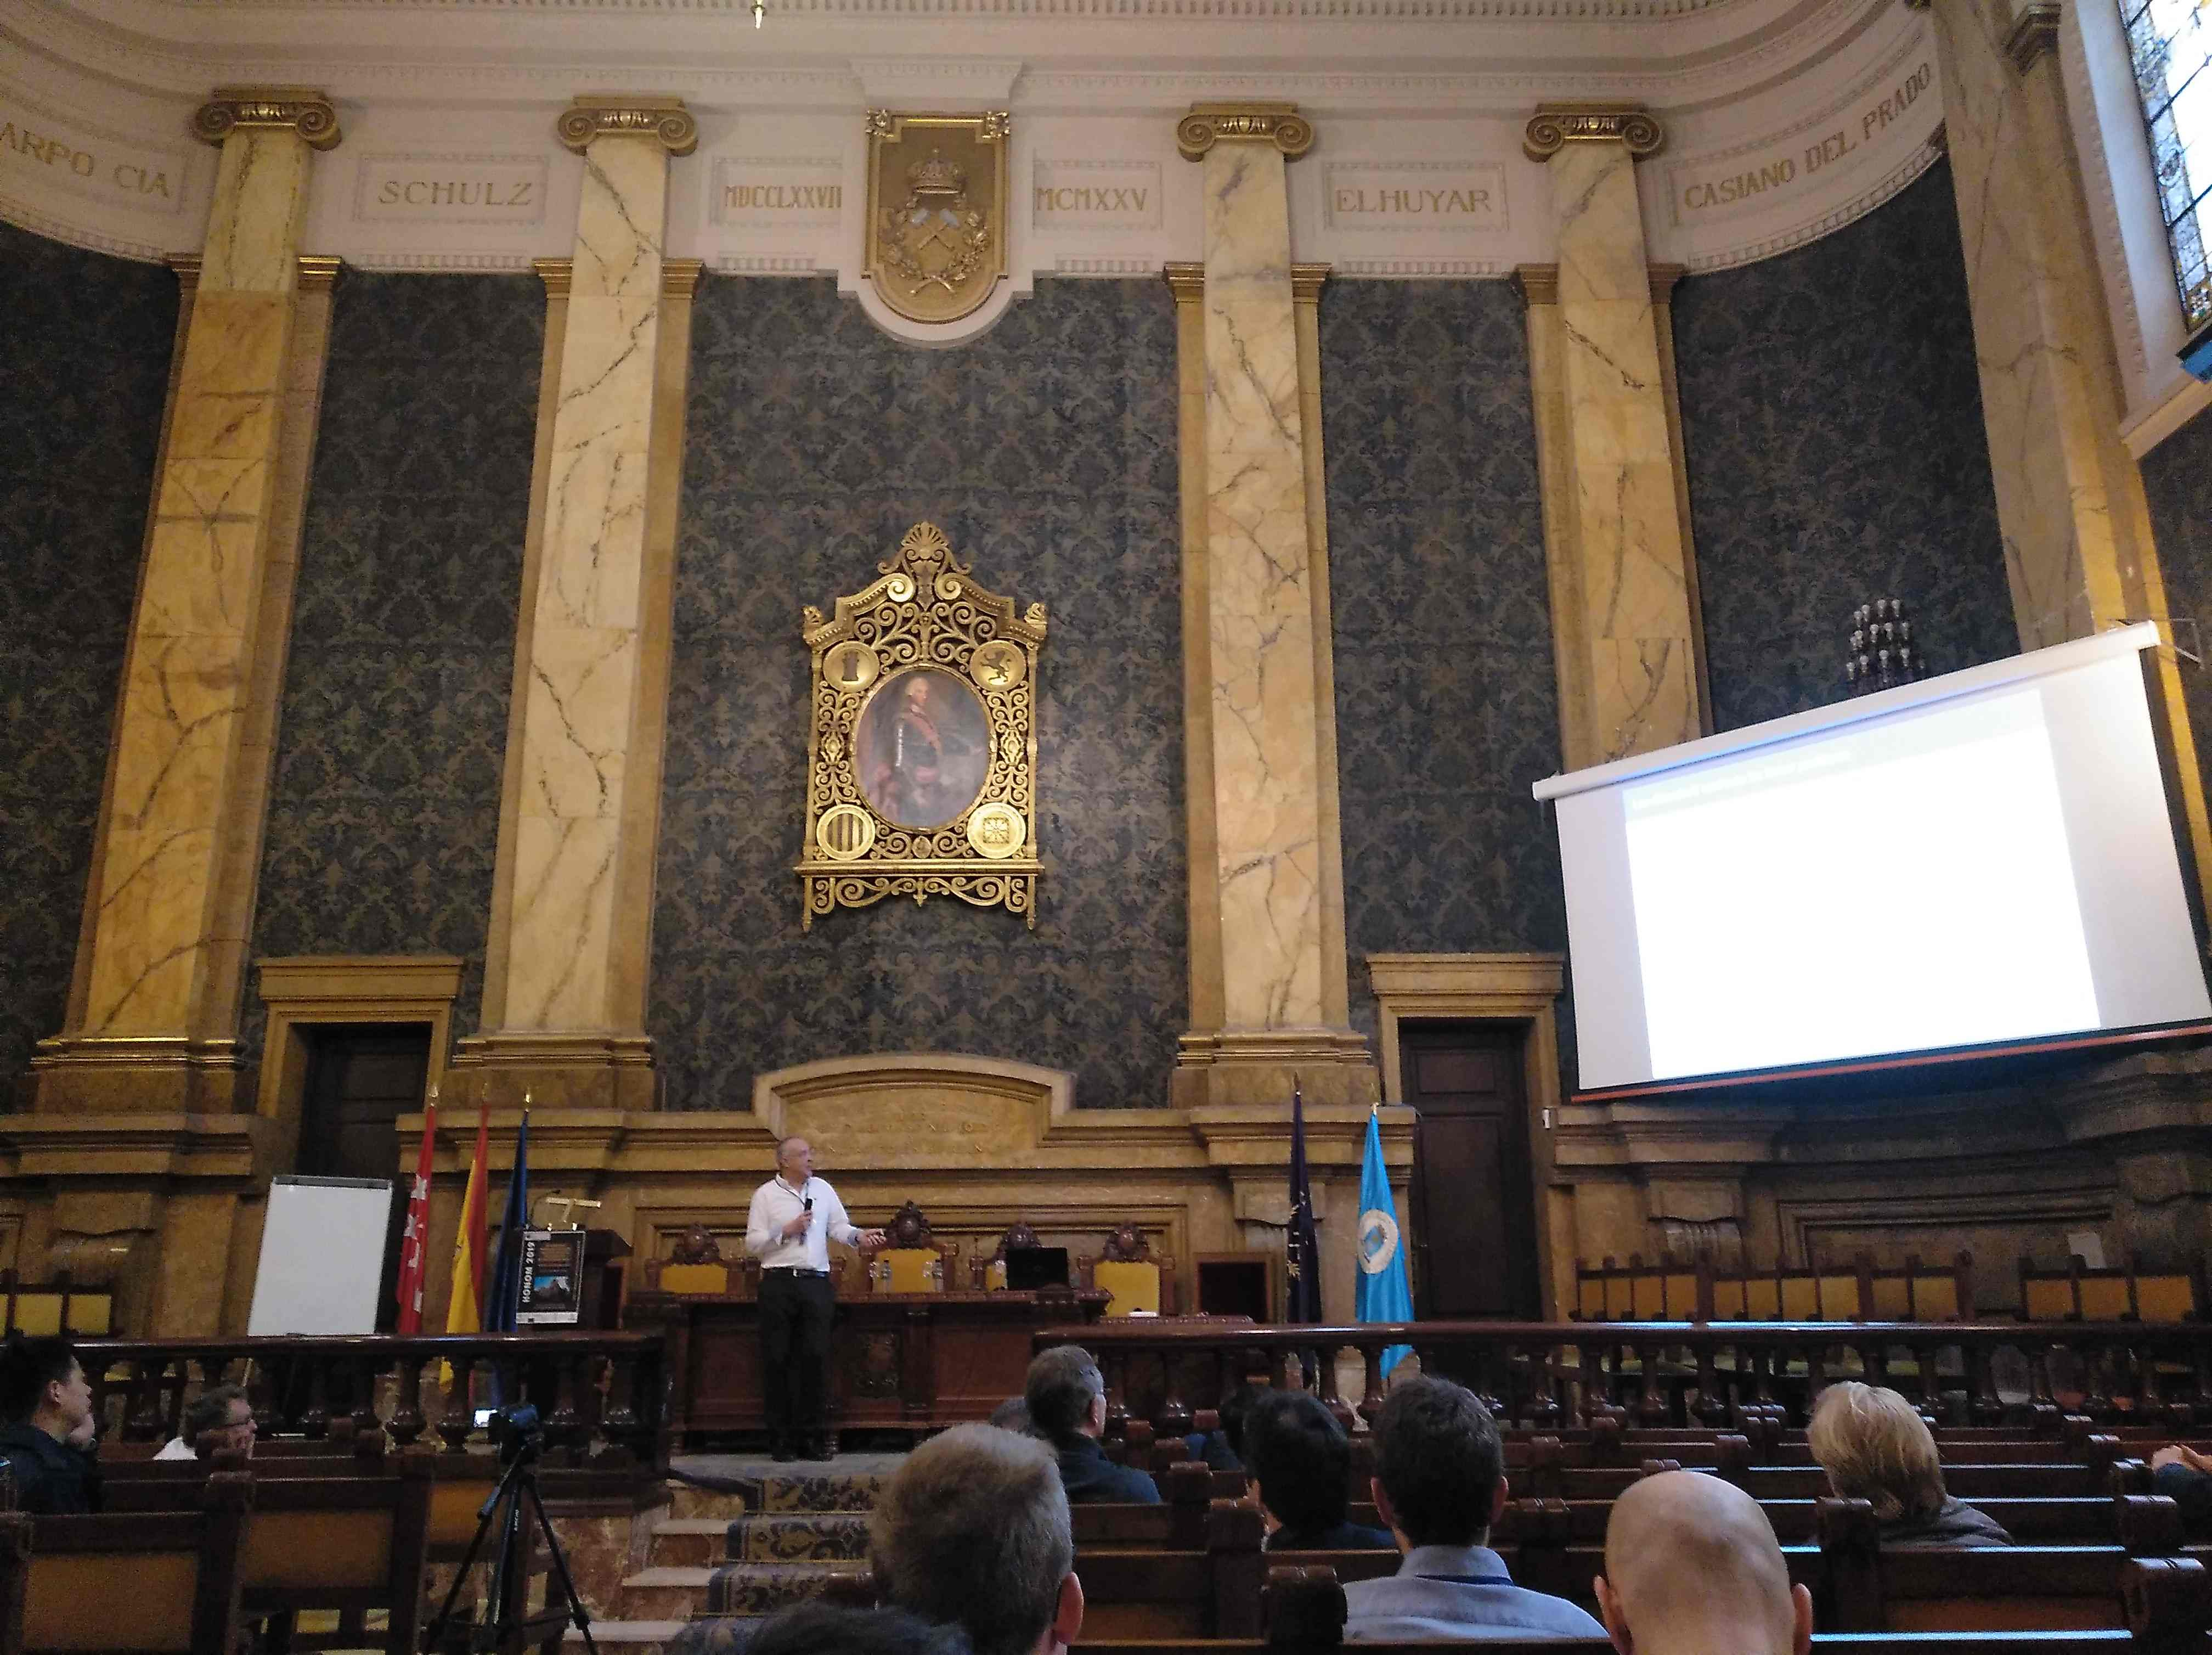
\includegraphics[width=0.9\textwidth]{CPares}
		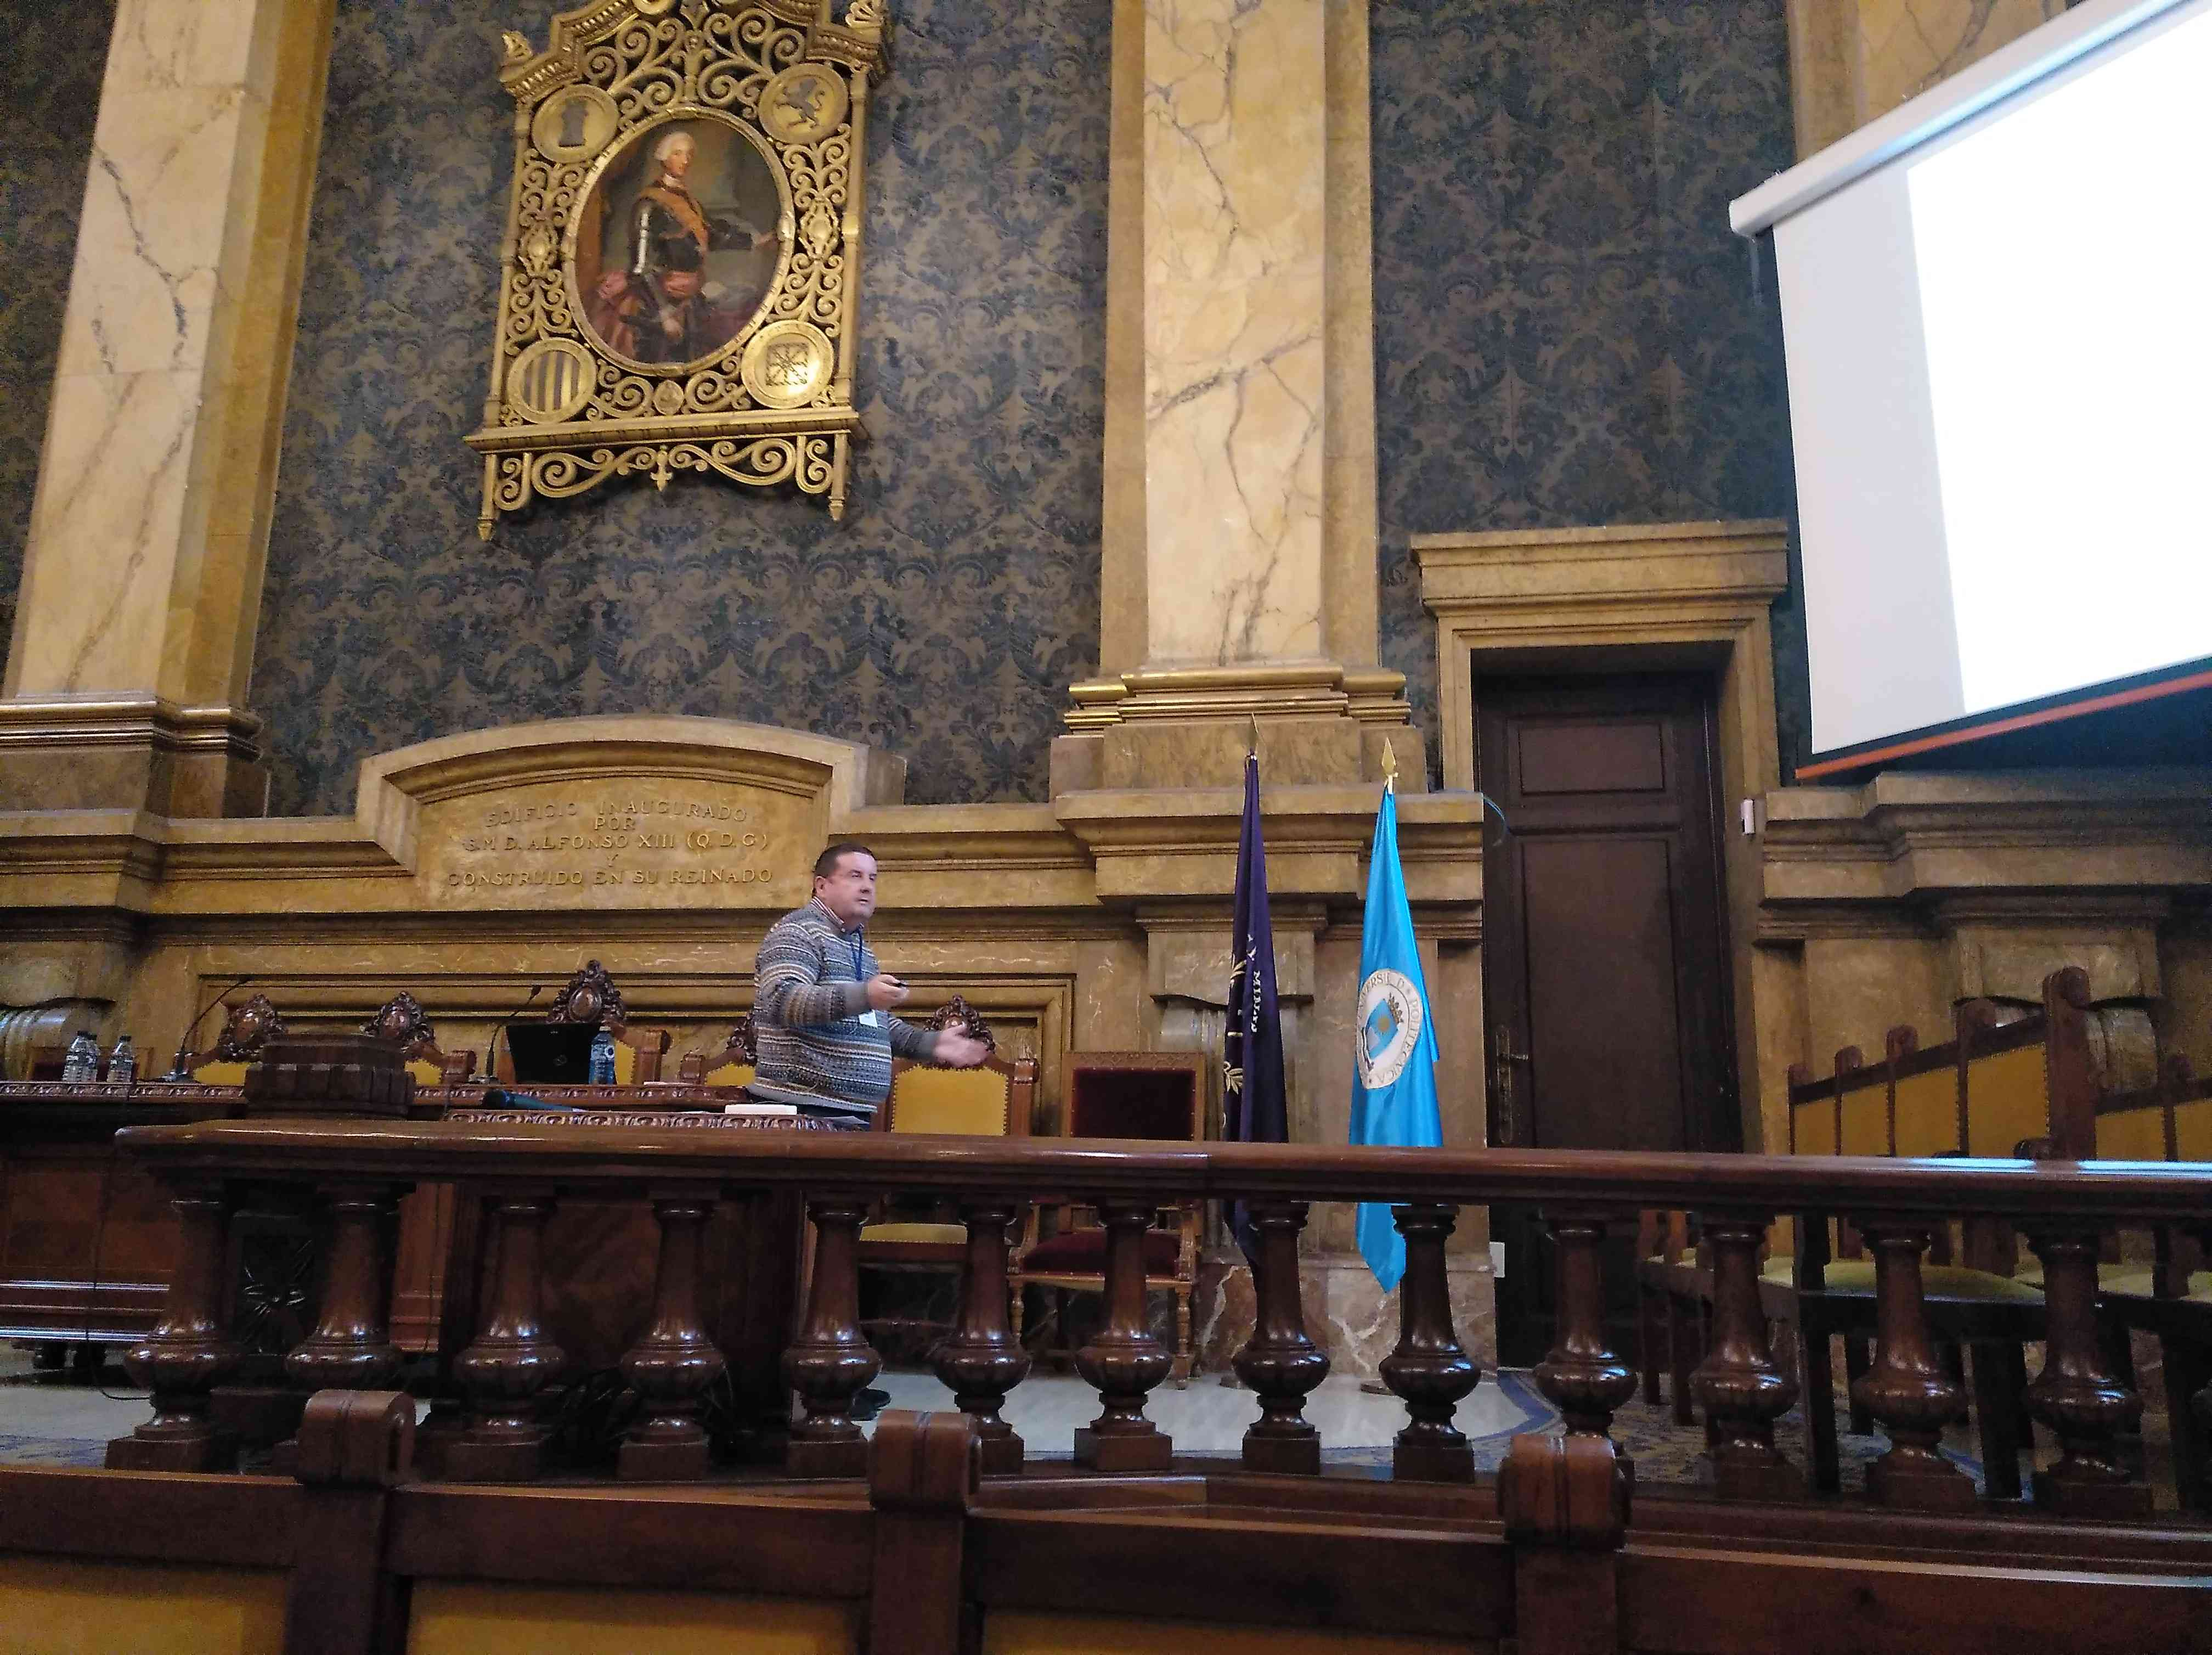
\includegraphics[width=0.9\textwidth]{APascau}
	\label{fig:Salon3}
	\caption{Imágenes de las charlas de Carlos Parés y Antonio Pascau en el Salón de Actos de la ETSIME  - Fuente: Comité Organizador}
\end{figure}
\end{center}
%
\begin{center}
\begin{figure}
	\centering
		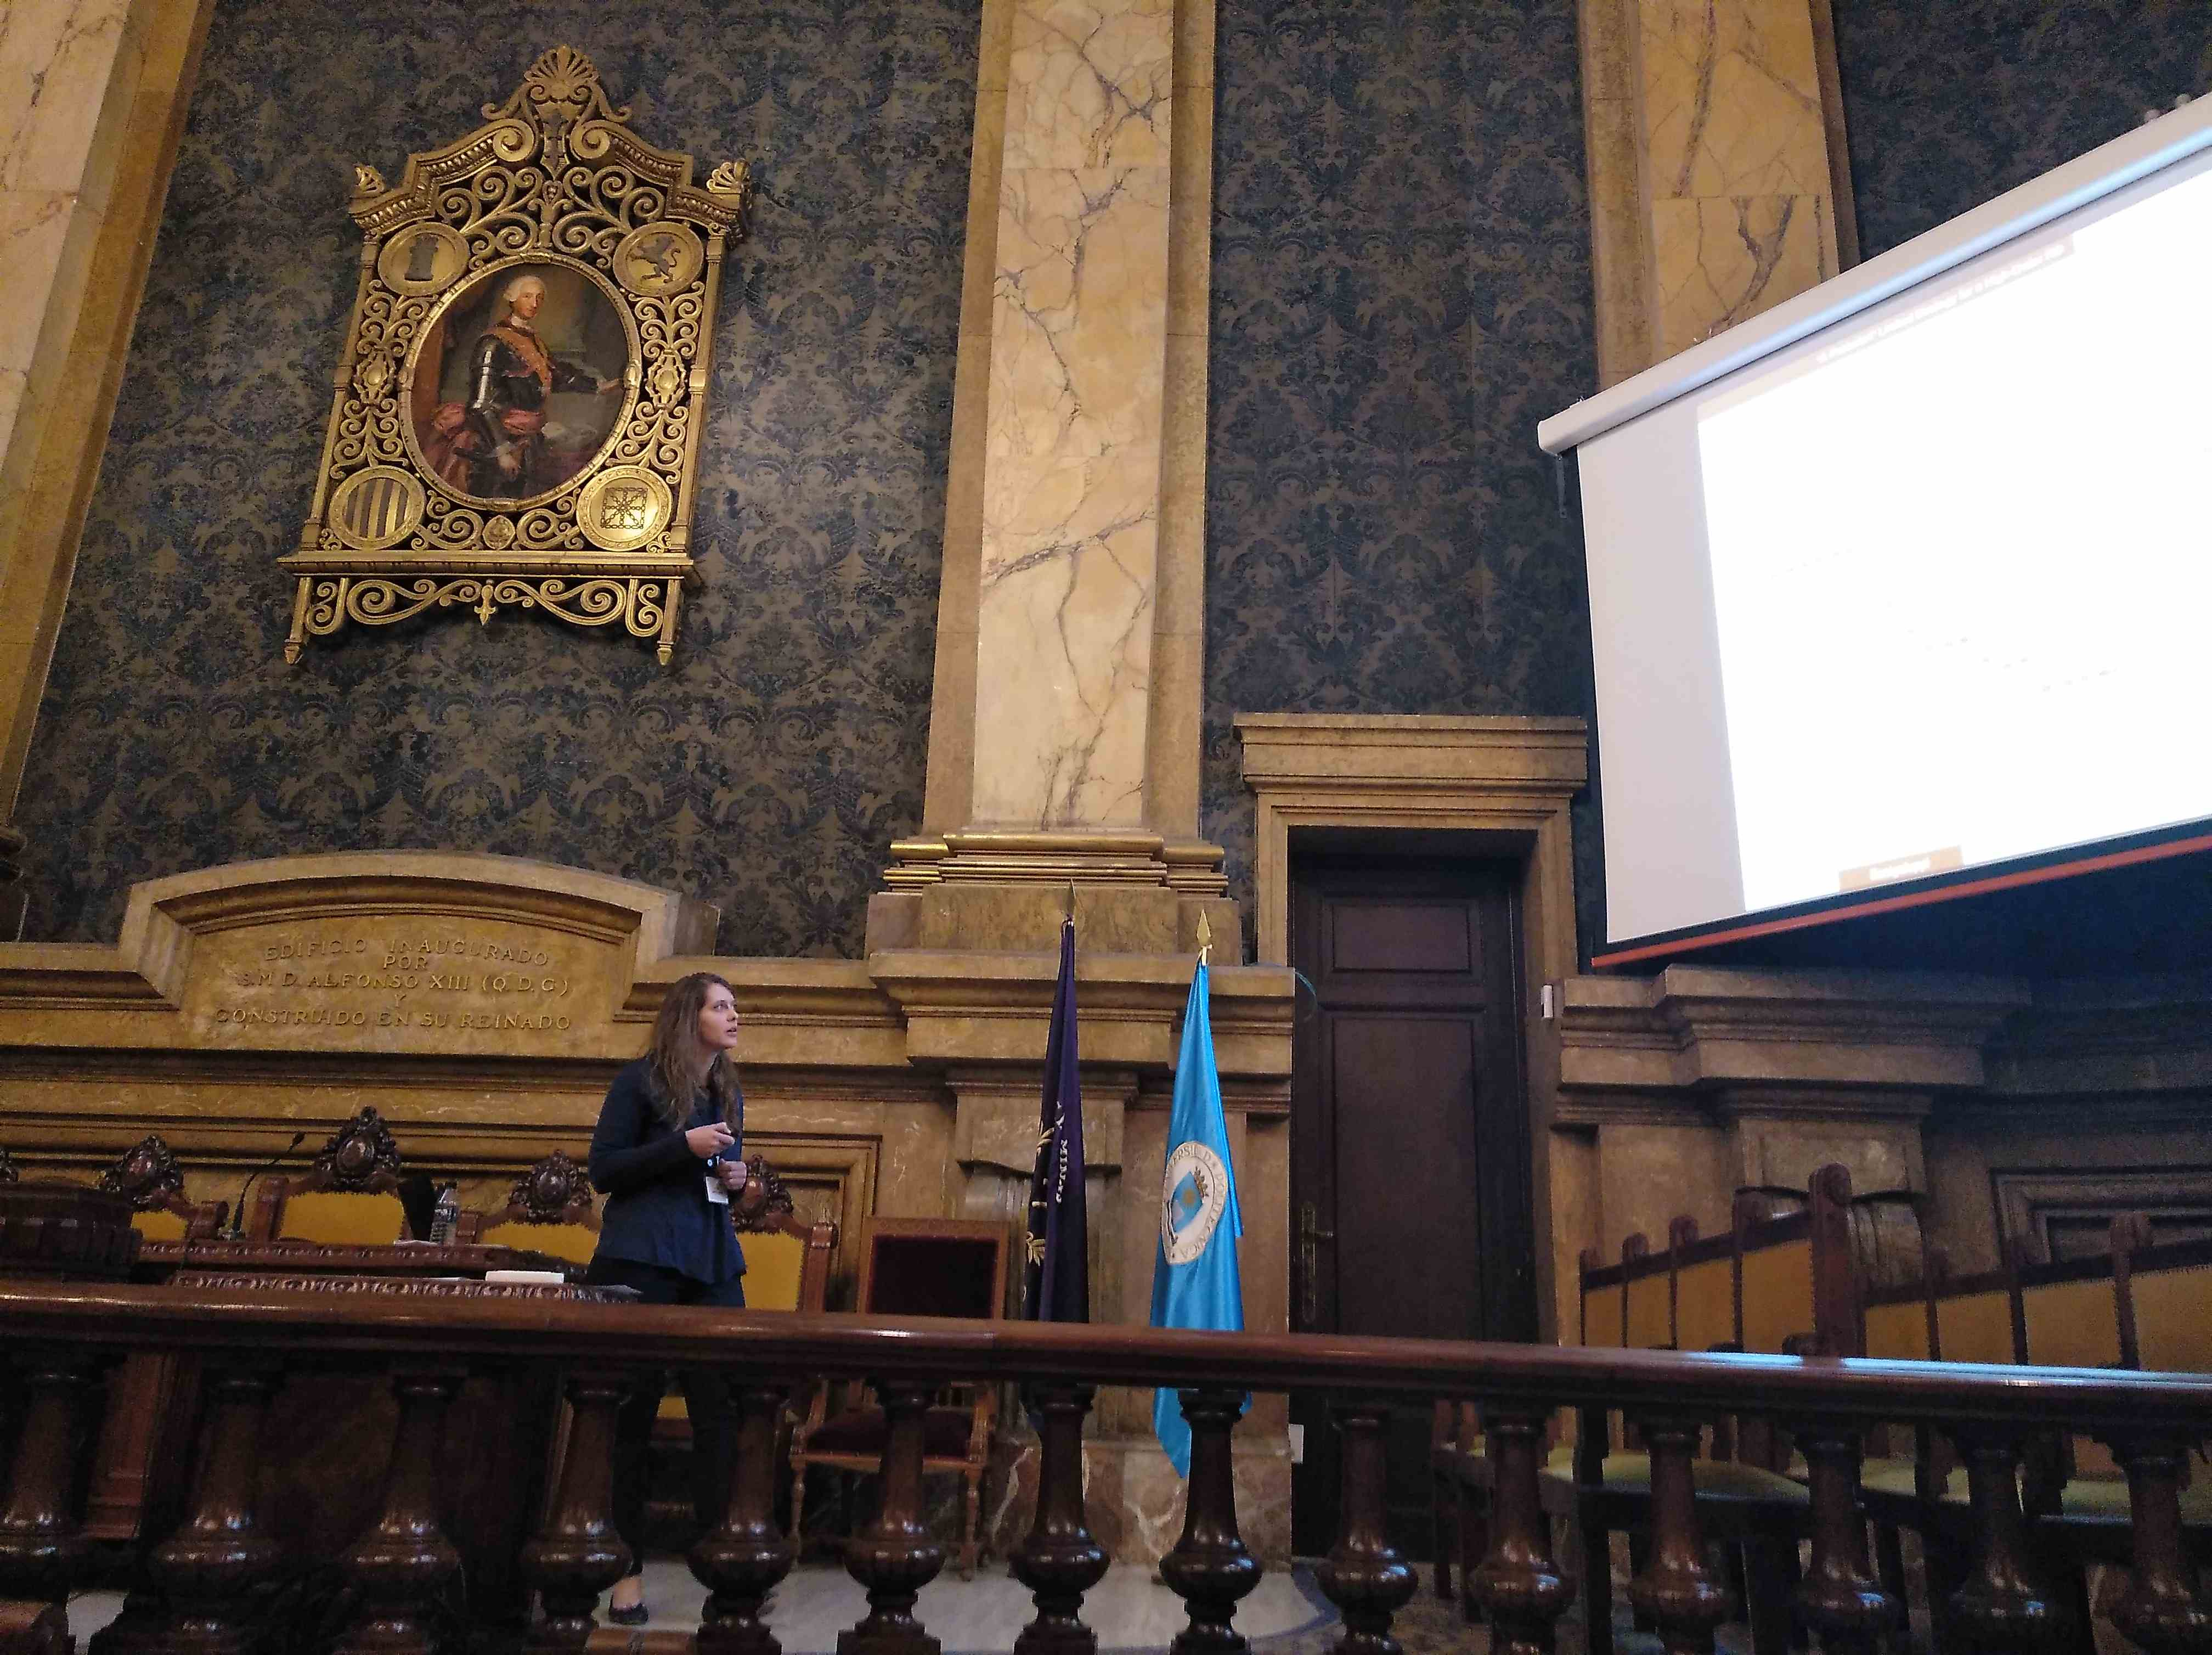
\includegraphics[width=0.9\textwidth]{PBacigaluppi}
		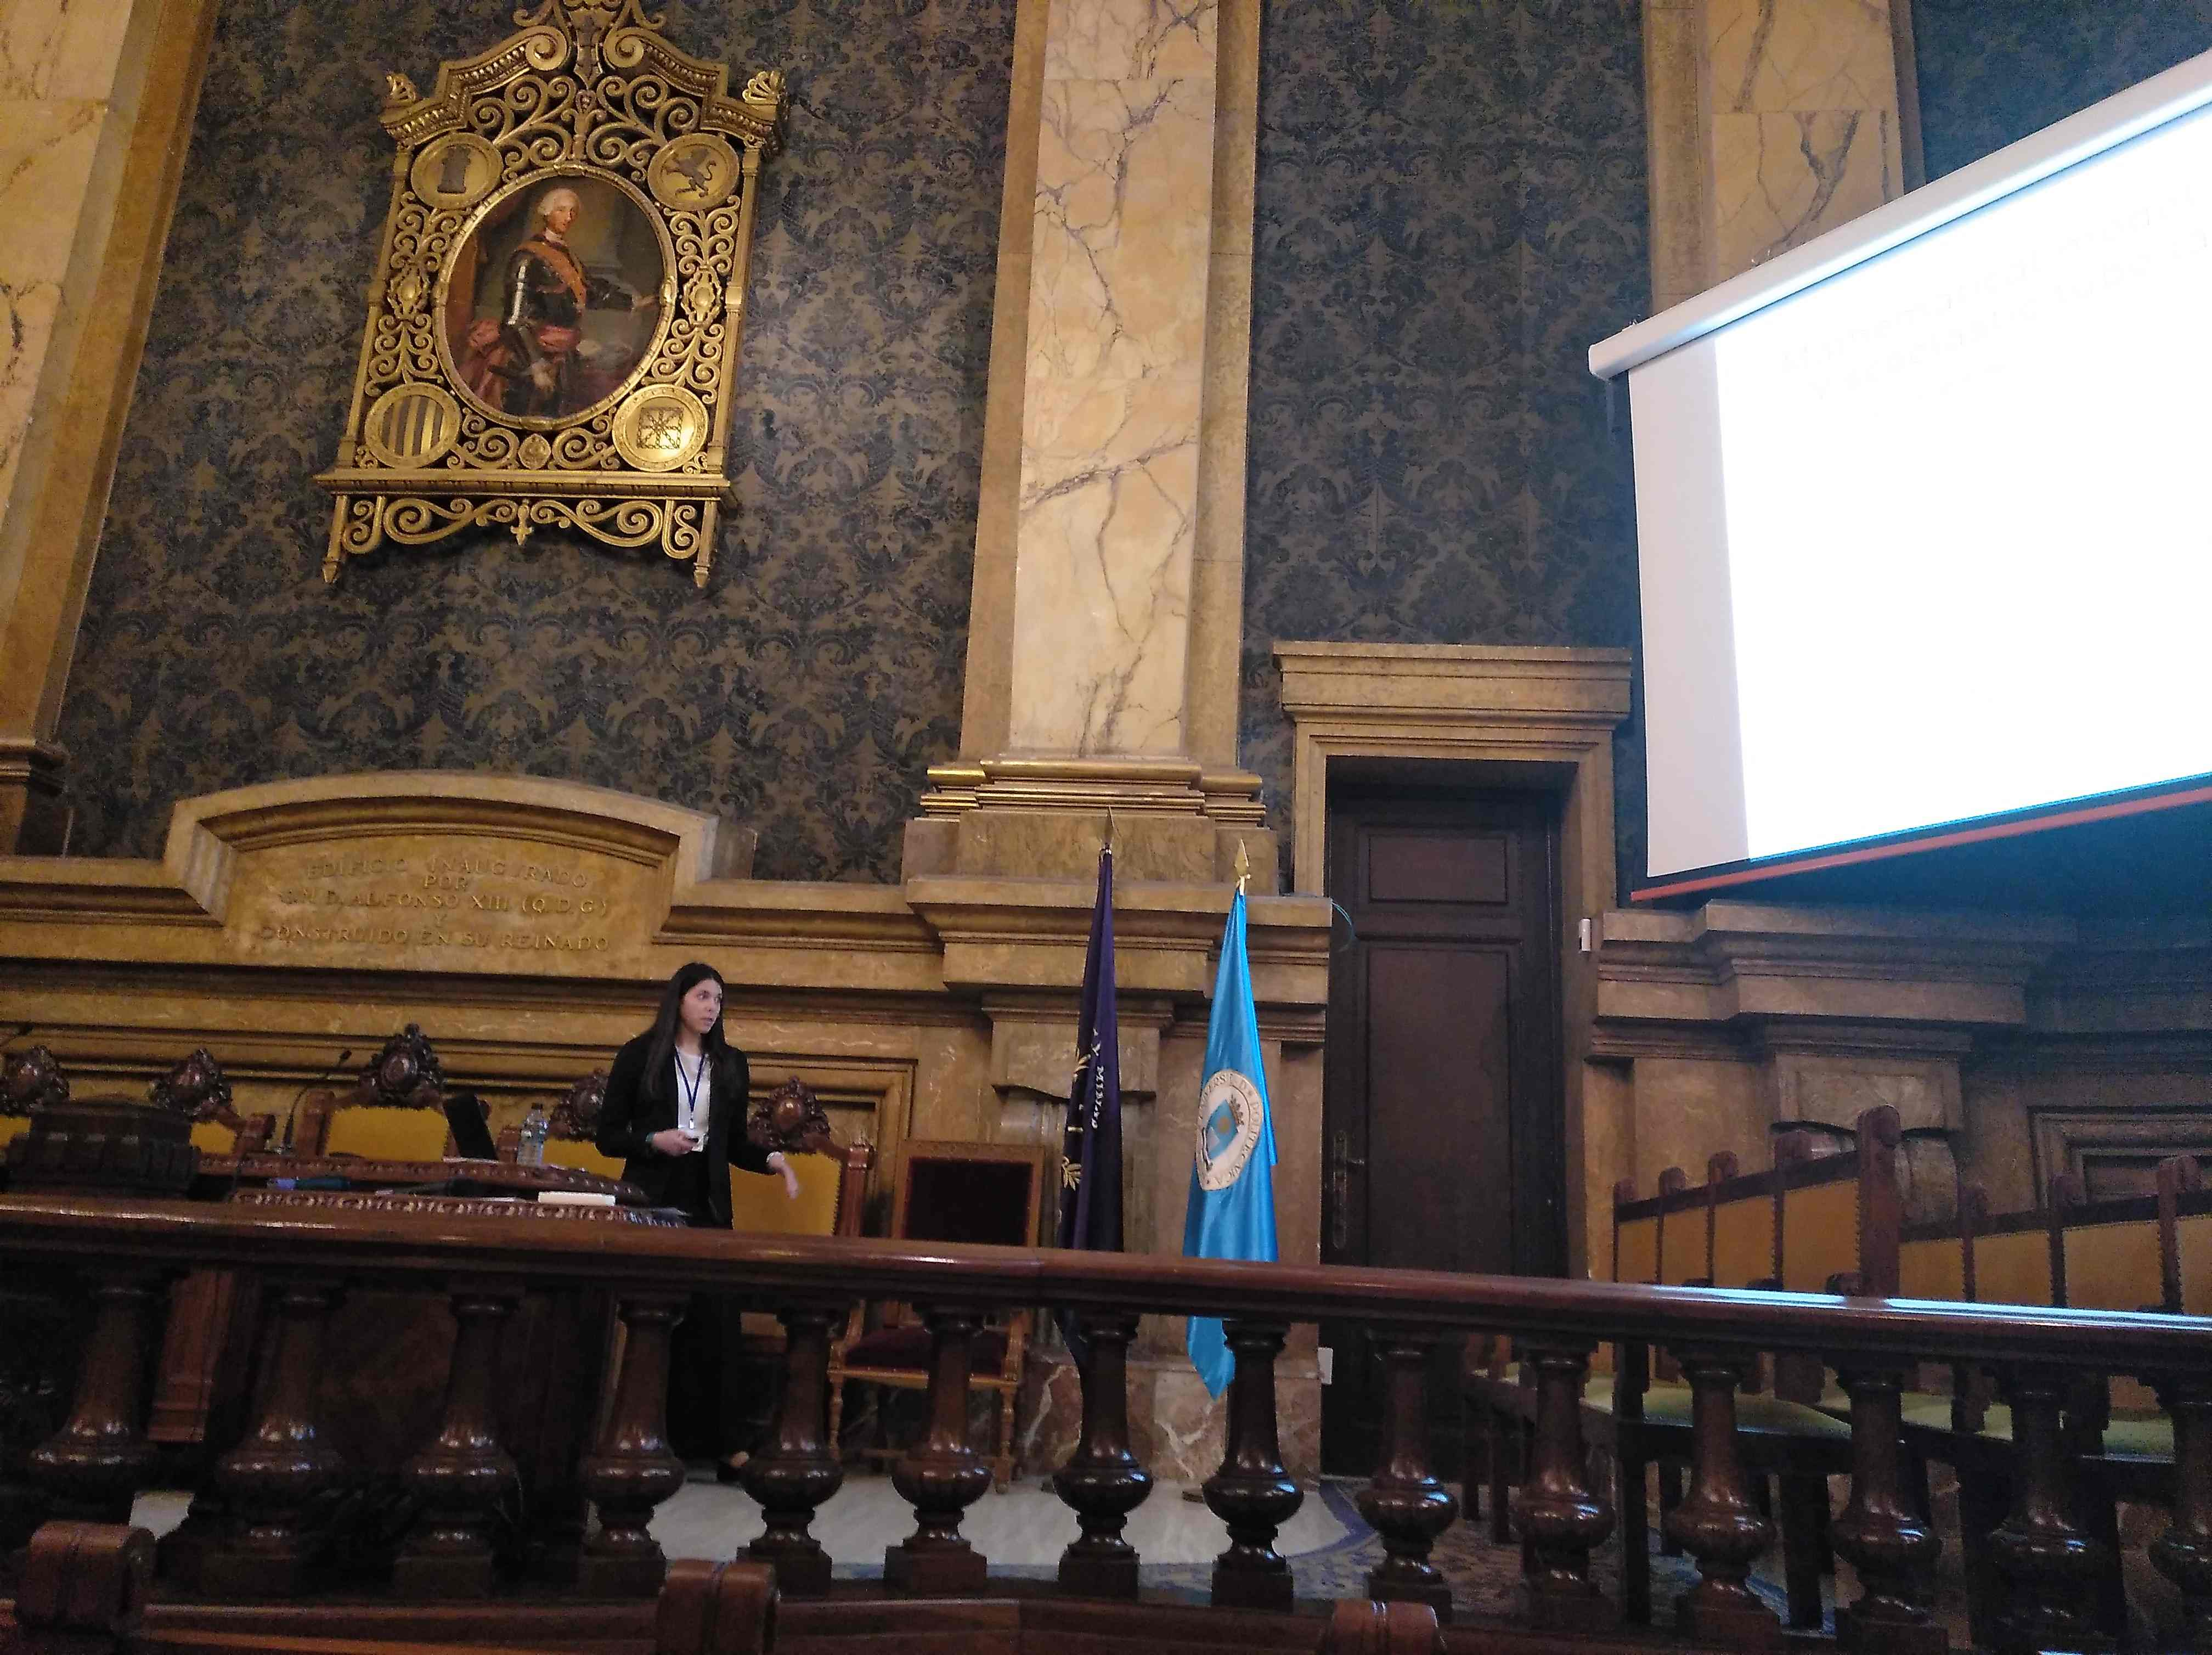
\includegraphics[width=0.9\textwidth]{GBertaglia}
	\label{fig:Salon4}
	\caption{Imágenes sesiones paralelas en el Salón de Actos de la ETSIME (P. Bacigaluppi y G. Bertaglia)  - Fuente: Comité Organizador}
\end{figure}
\end{center}
%
\begin{center}
\begin{figure}
	\centering
		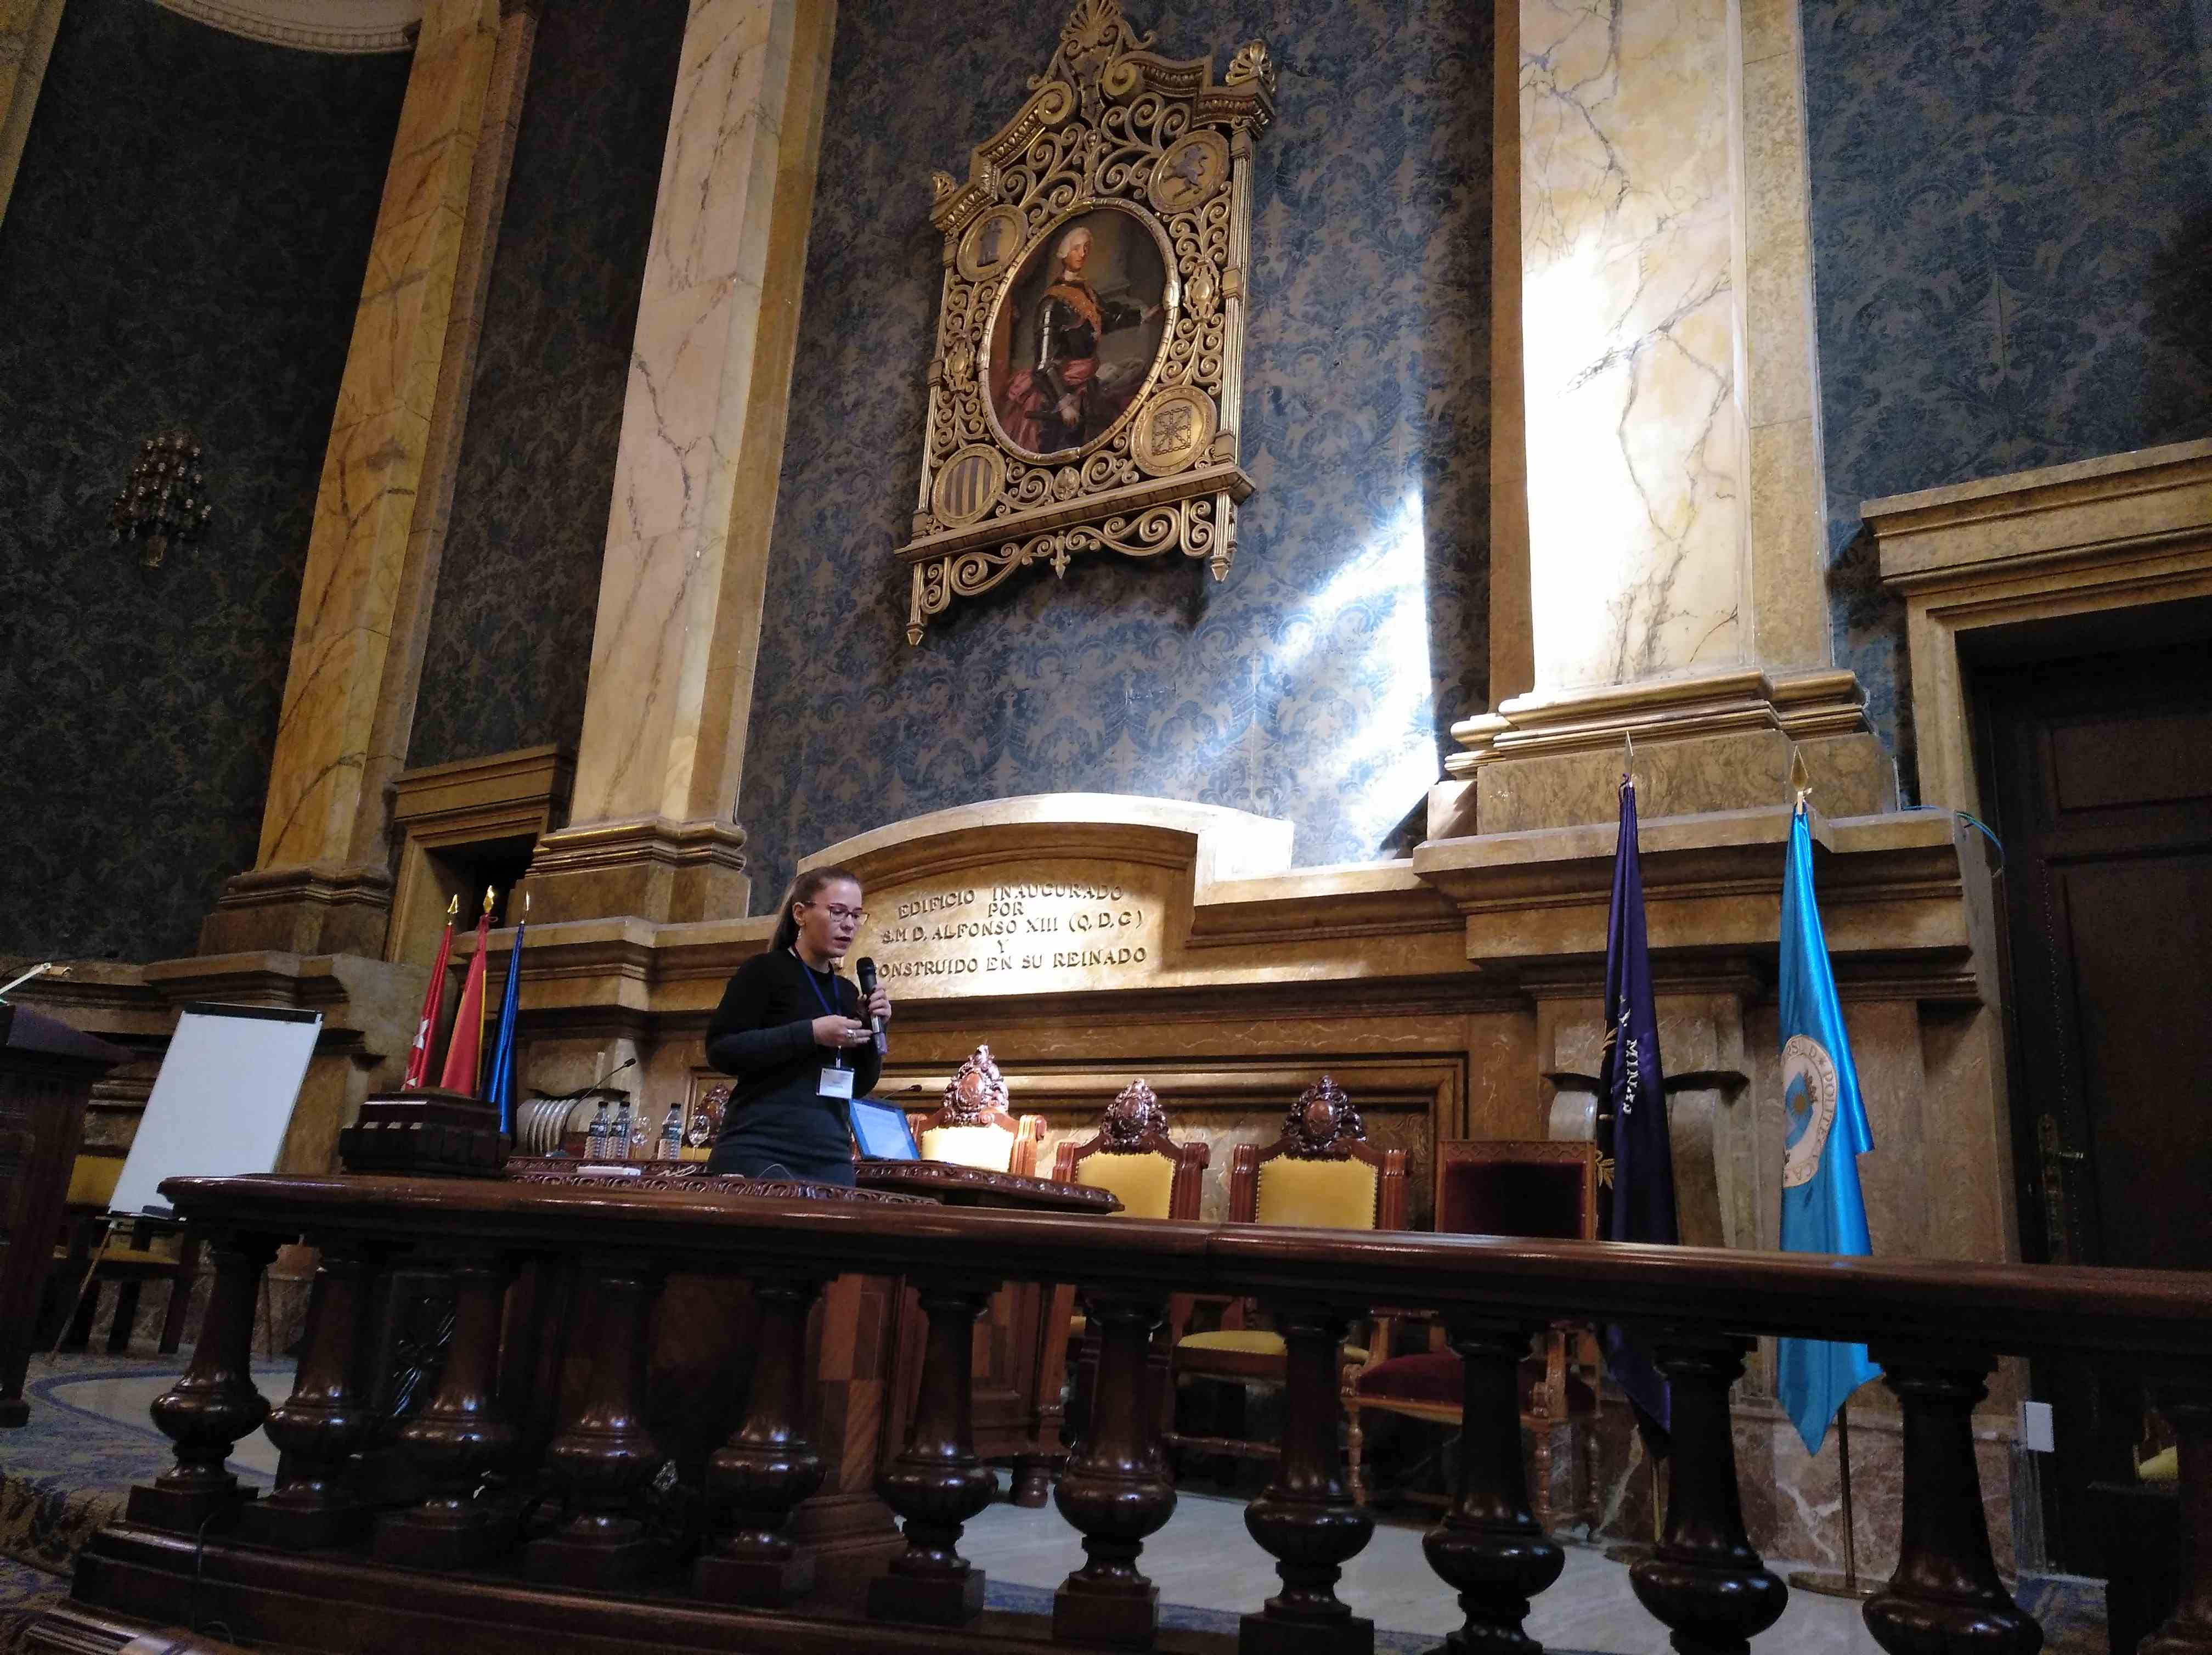
\includegraphics[width=0.9\textwidth]{Laura_Saavedra}
		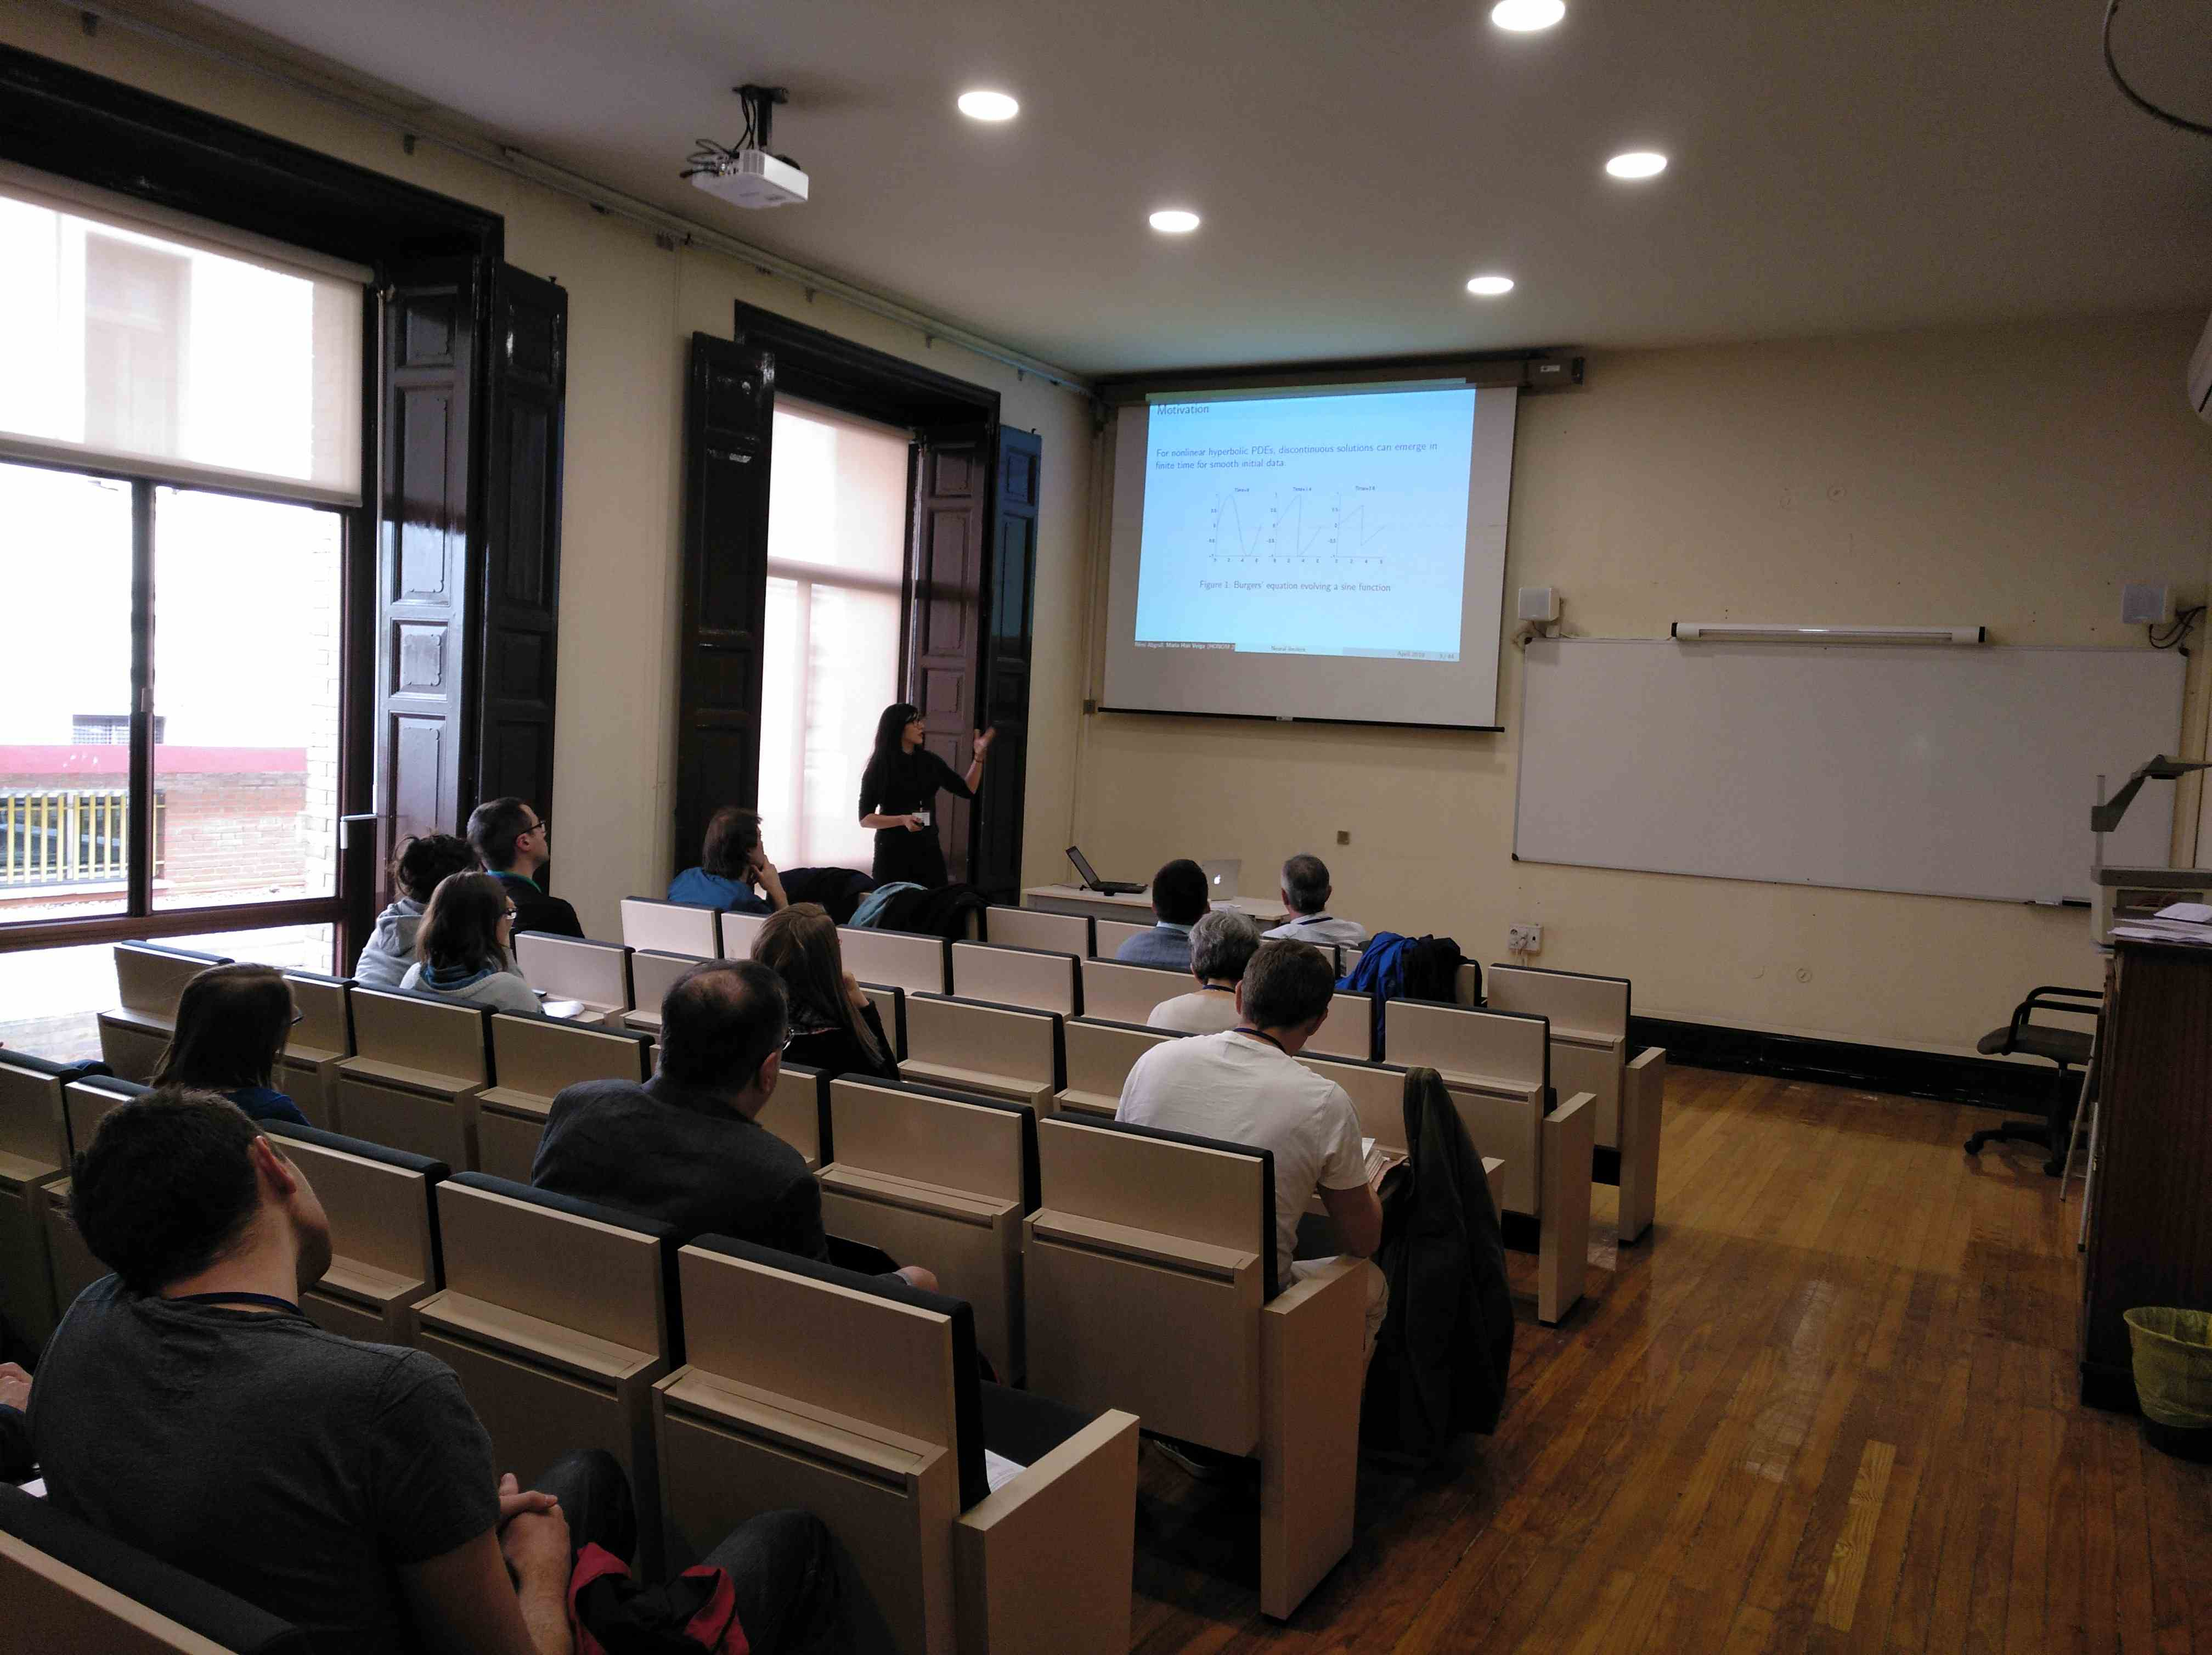
\includegraphics[width=0.9\textwidth]{Maria_Han}
	\label{fig:Salon5}
	\caption{Imágenes de las charlas de Laura Saavedra y Maria Han Veiga  - Fuente: Comité Organizador}
\end{figure}
\end{center}
%
Al final de cada día tenía lugar una discusión en grupo donde se debatía con todos los conferenciantes en la jornada sobre los temas tratados en la misma. En un ambiente tranquilo y relajado se desarrollaba una discusión entre los conferenciantes y los participantes aclarando cuestiones o analizando posibles alternativas a los problemas planteados y los métodos numéricos aplicados.
%
\begin{center}
\begin{figure}
	\centering
		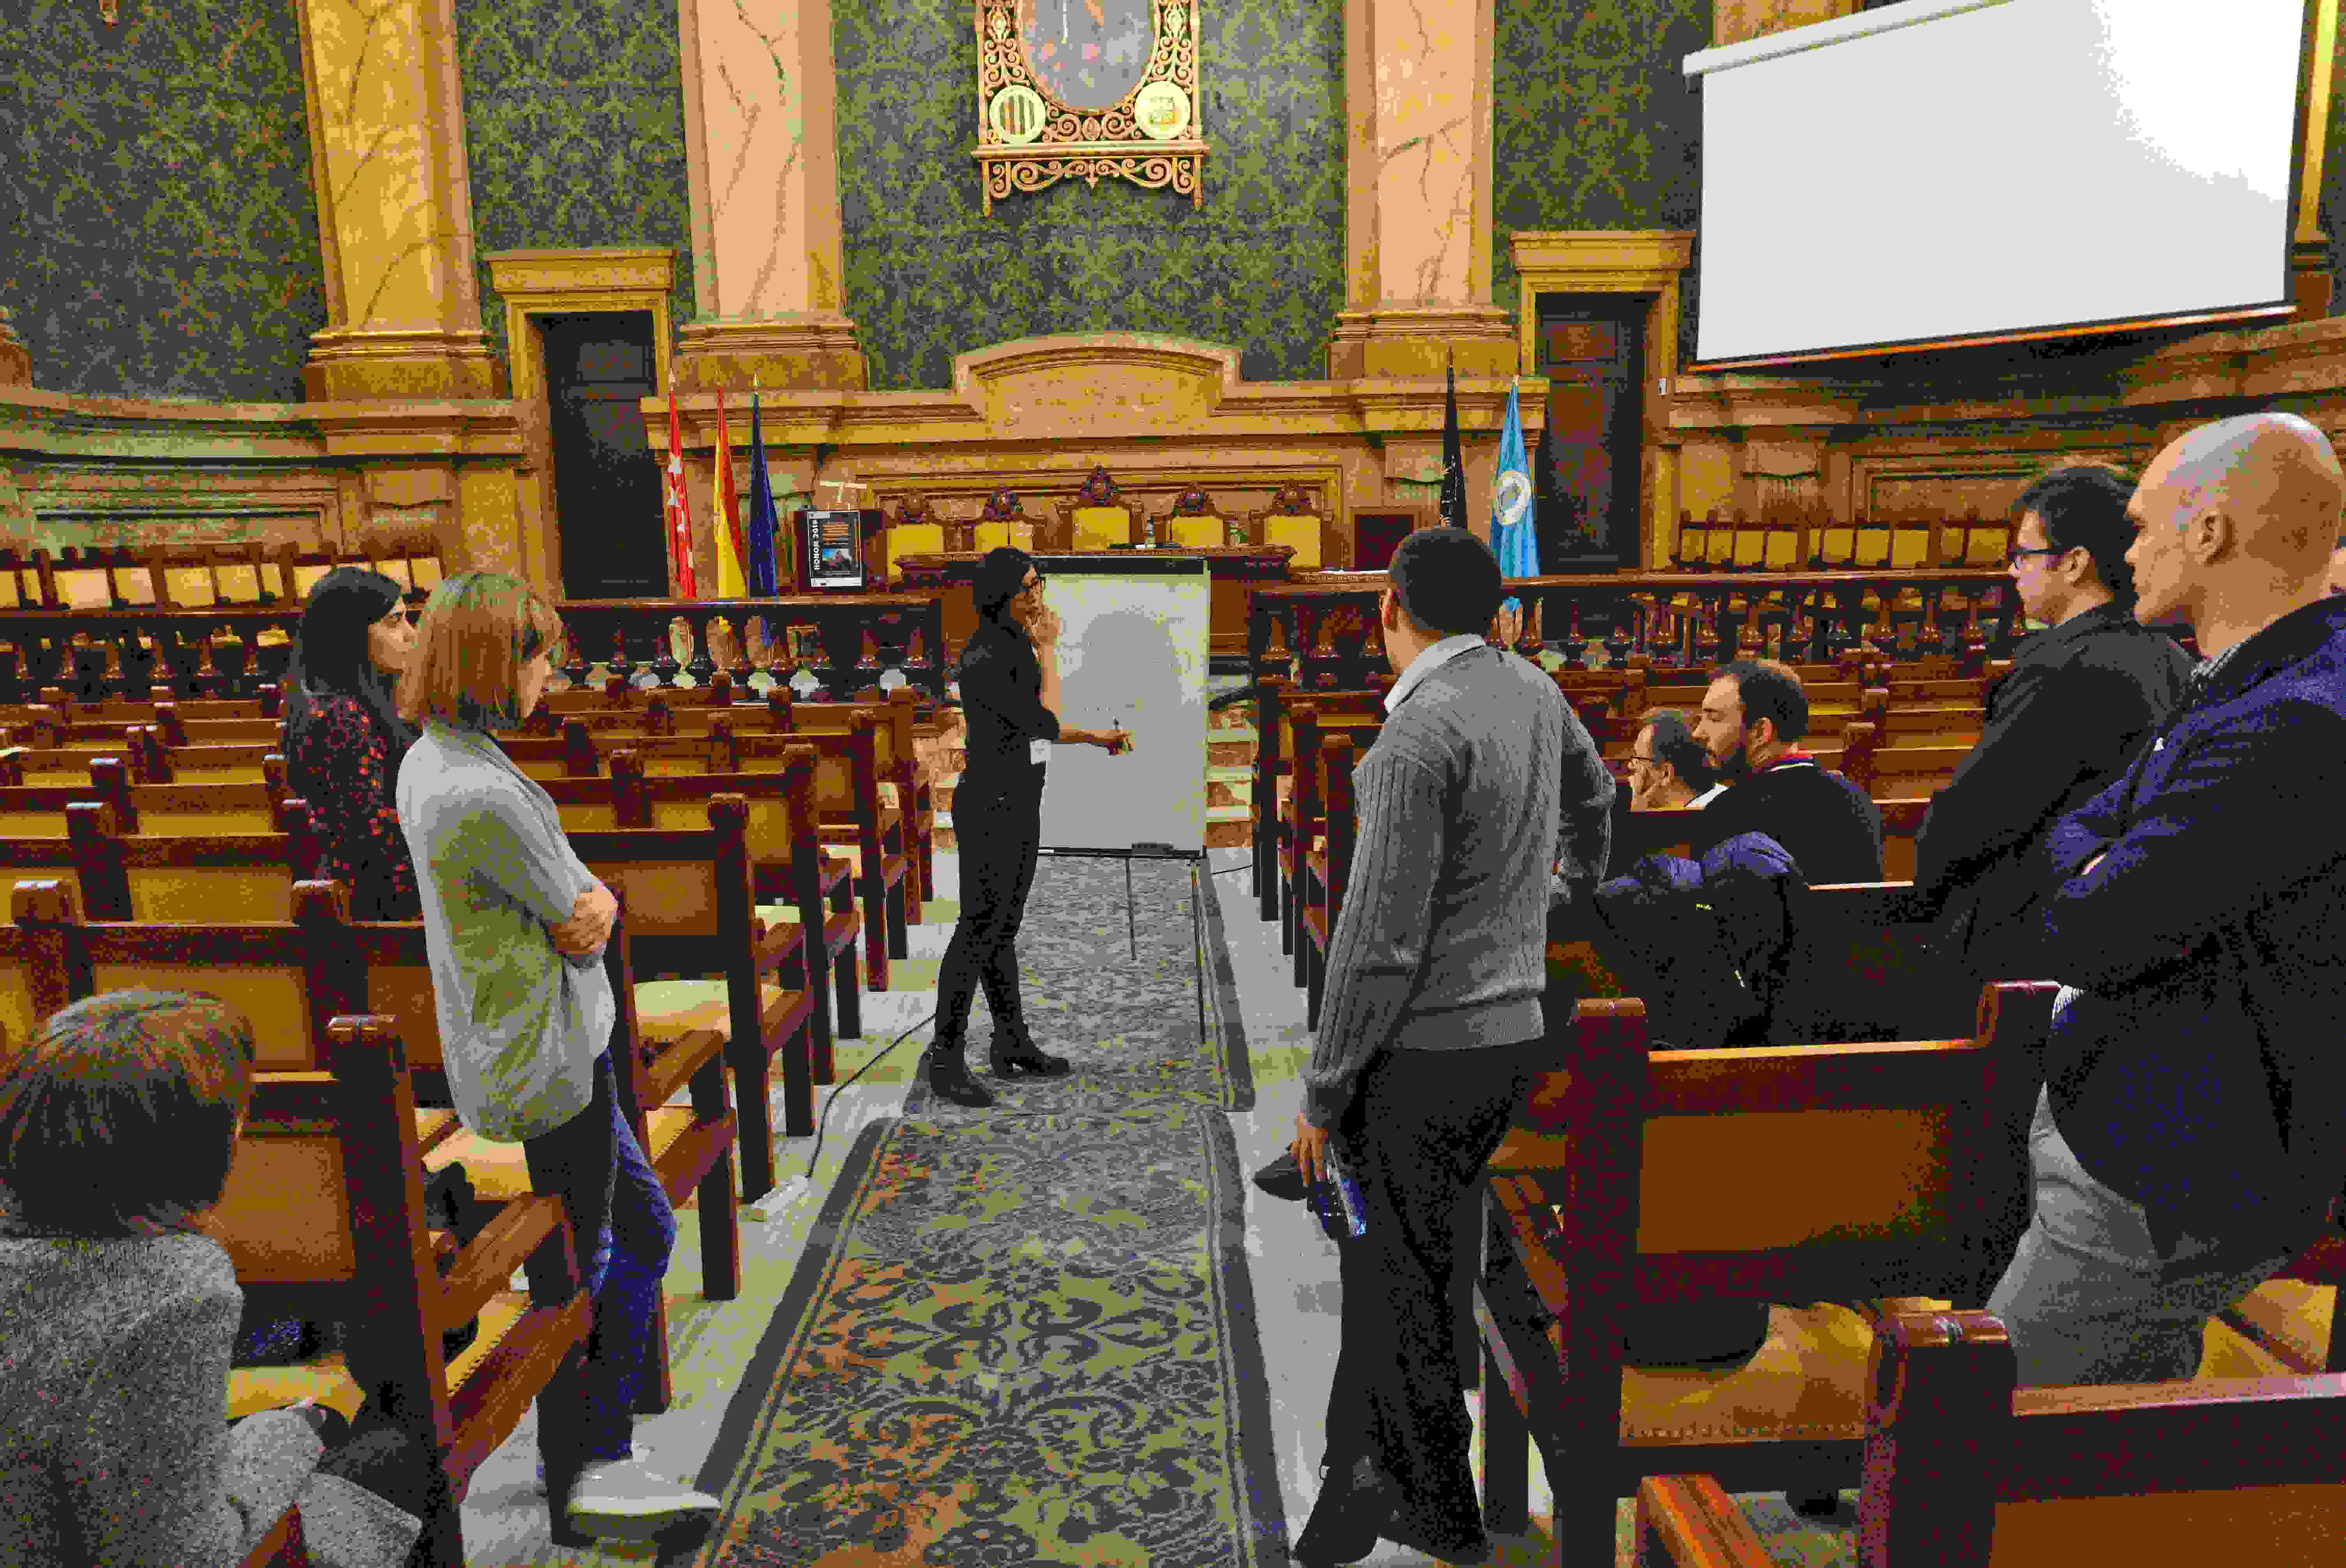
\includegraphics[width=.95\textwidth]{GroupDiscussion}
	\label{fig:Discussion}
	\caption{Escena de una de las discusiones en grupo en el Salón de Actos de la Escuela - Fuente: A. Baeza}
\end{figure}
\end{center}


\subsection{Actividades sociales}

El lunes 1 de abril tuvo lugar recepción en el Patio de Columnas de la ETSI de Minas y Energía donde se ofreció un cóctel de bienvenida a todos los participantes en el congreso. El siguiente día, martes 2 de abril, se organizó una visita guiada a la mina experimental Marcelo Jorissen y al museo histórico-minero. La mina se encuentra situada en el recinto de la Escuela y fue creada por uno de los antiguos directores de la Escuela, Marcelo Jorissen, en el año 1967 y, si bien es experimental, todos sus elementos proceden de minas reales y representa una auténtica mina de carbón. La visita fue dirigida por el profesor Juan Herrera quien explicó a los participantes los detalles de la misma. El miércoles 3 de abril se desarrolló una visita guiada al Museo del Prado junto con un recorrido panorámico por el centro de Madrid. Fue una actividad de gran interés para los participantes, pues les dio la oportunidad de recorrer un museo de gran valor histórico y artístico, reconocido como uno de los museos más importantes del mundo y más visitados. Para esta actividad se contó con dos autobuses para el transporte y dos guías profesionales en inglés. La Cena del Congreso tuvo lugar el jueves 4 de abril. Durante la misma, se anunció a los asistentes la próxima edición de HONOM, que se celebrará en Guimar$\tilde{a}$es (Portugal) en 2021. Ese mismo día, antes de la cena, se tomó la foto de grupo en la puerta principal de la Escuela. 
%
\begin{center}
\begin{figure}
	\centering
		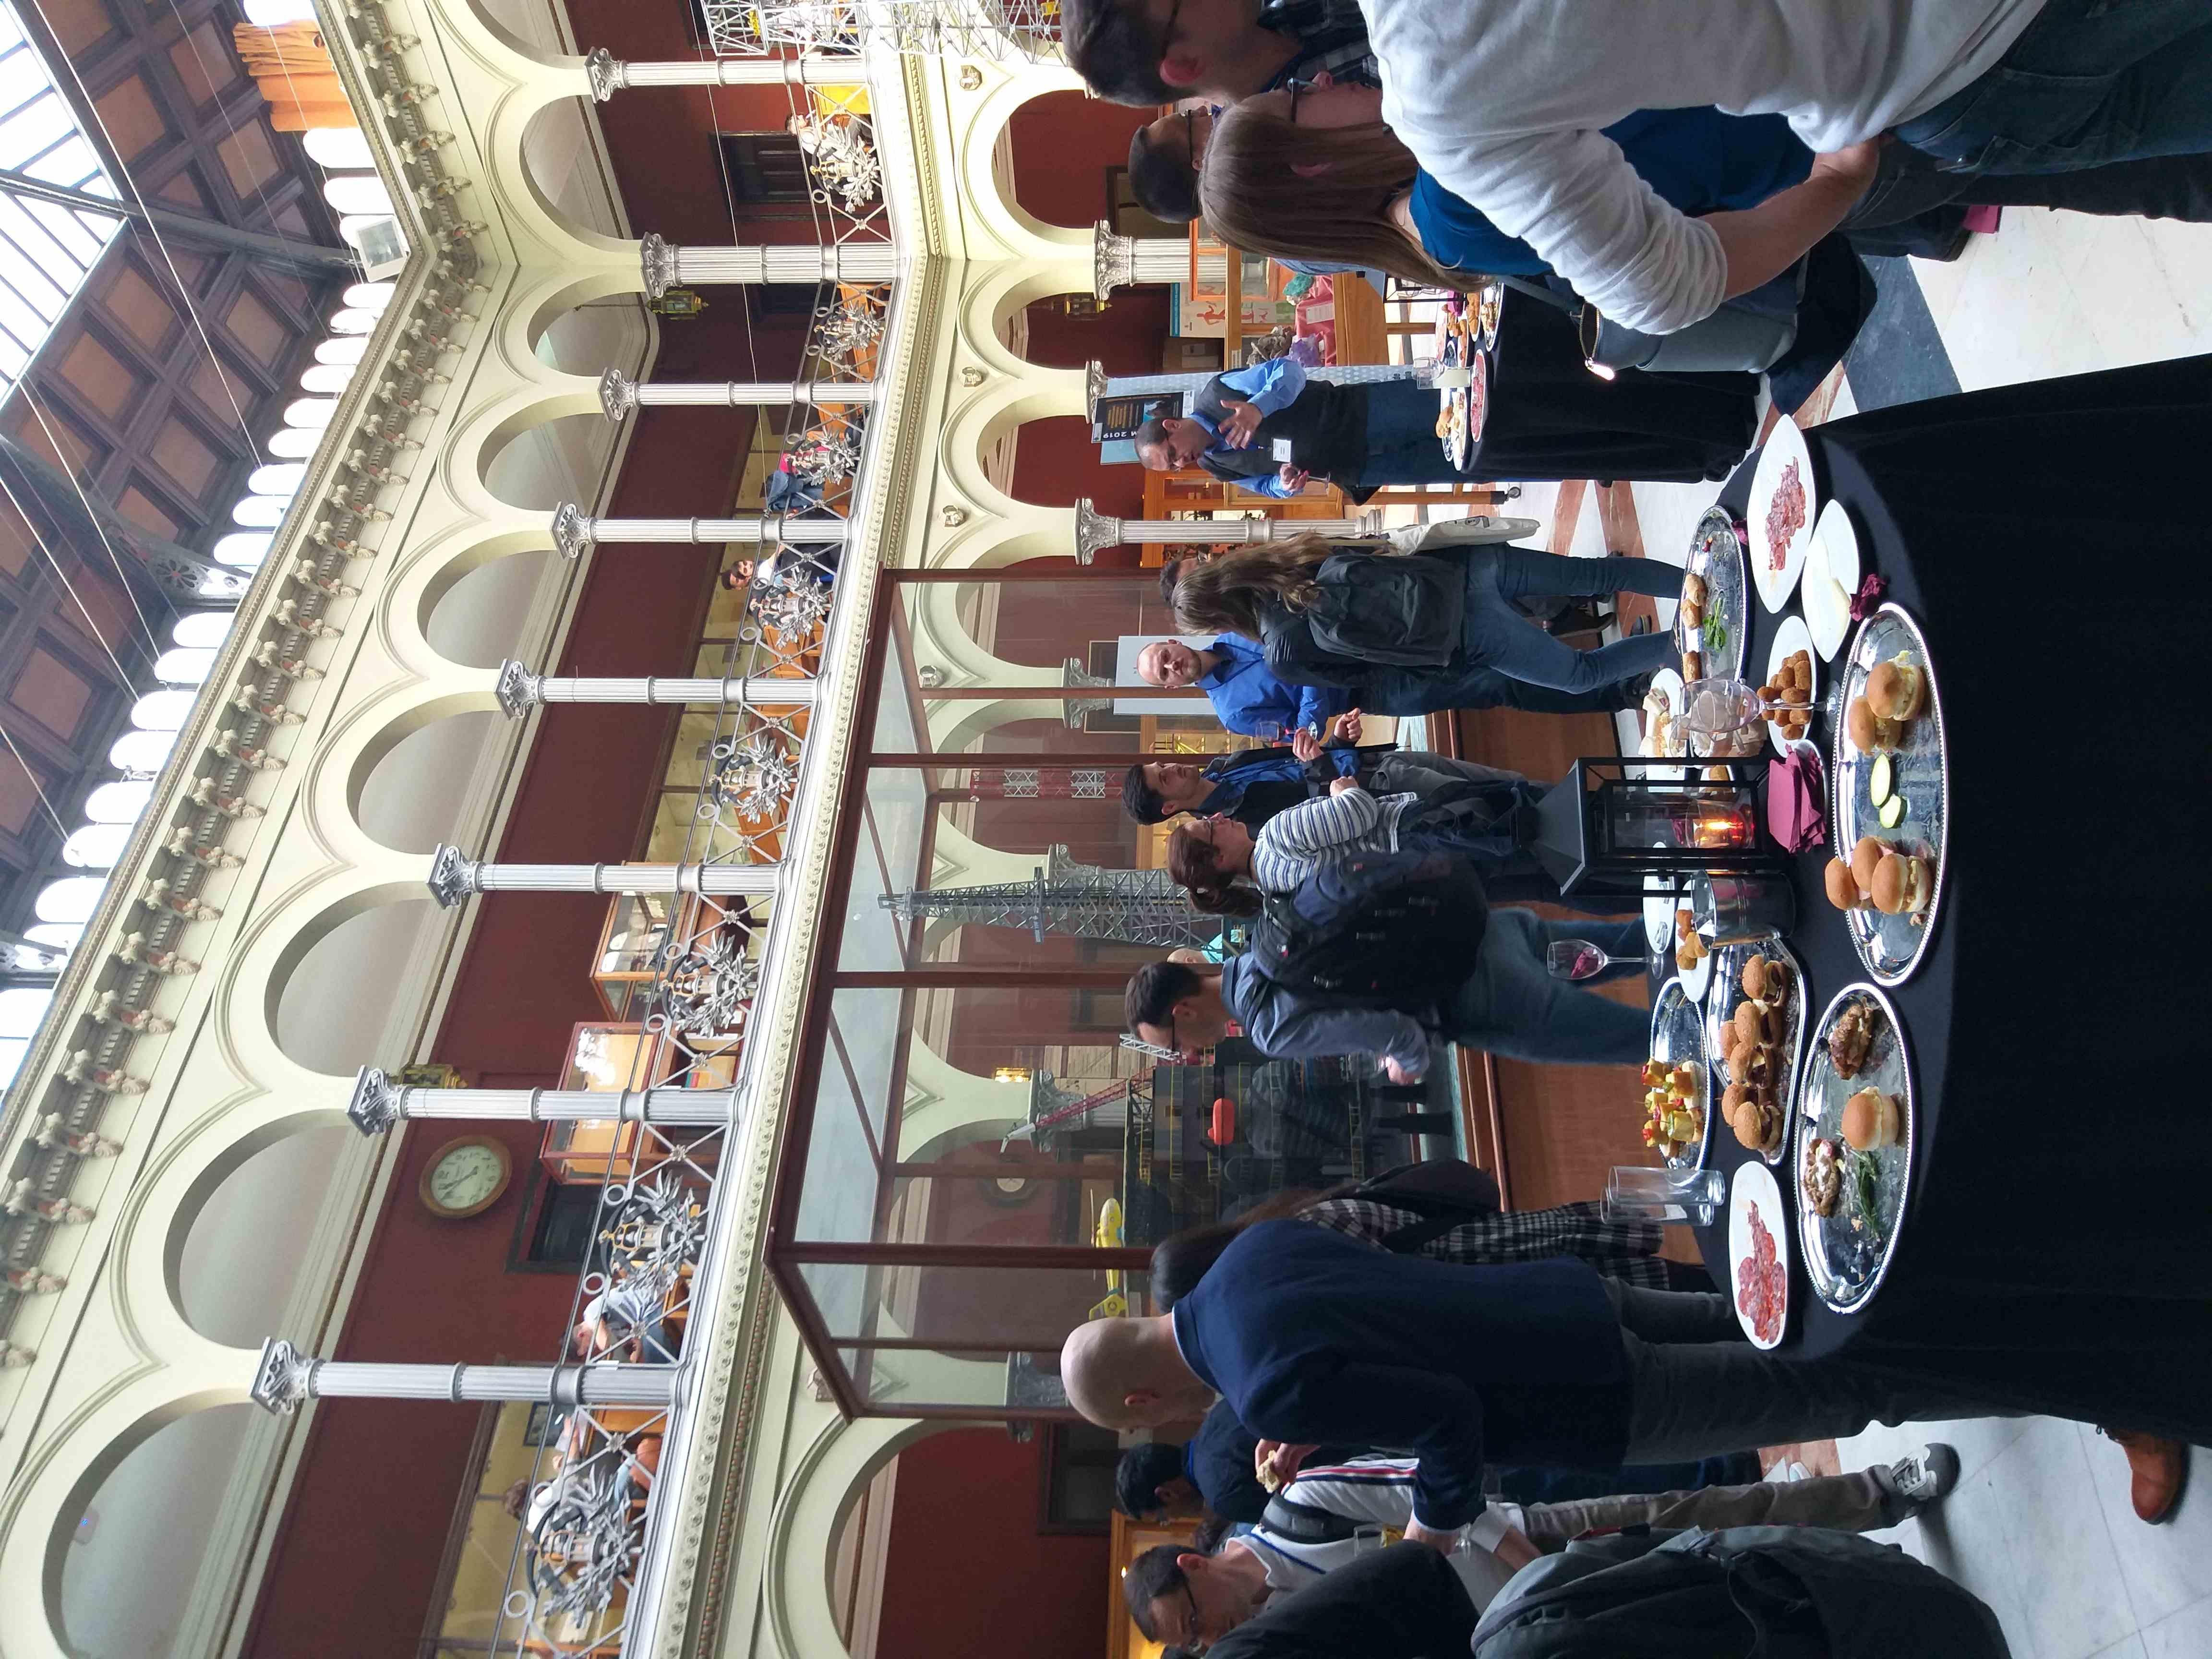
\includegraphics[width=.95\textwidth, angle=270]{Recepcion}
	\label{fig:RecepcionFoto}
	\caption{Recepeción en el Patio de Columnas de la Escuela - Fuente: Comité Organizador}
\end{figure}
\end{center}
%
\begin{center}
\begin{figure}
	\centering
		\includegraphics[width=.95\textwidth]{minaJuan}
		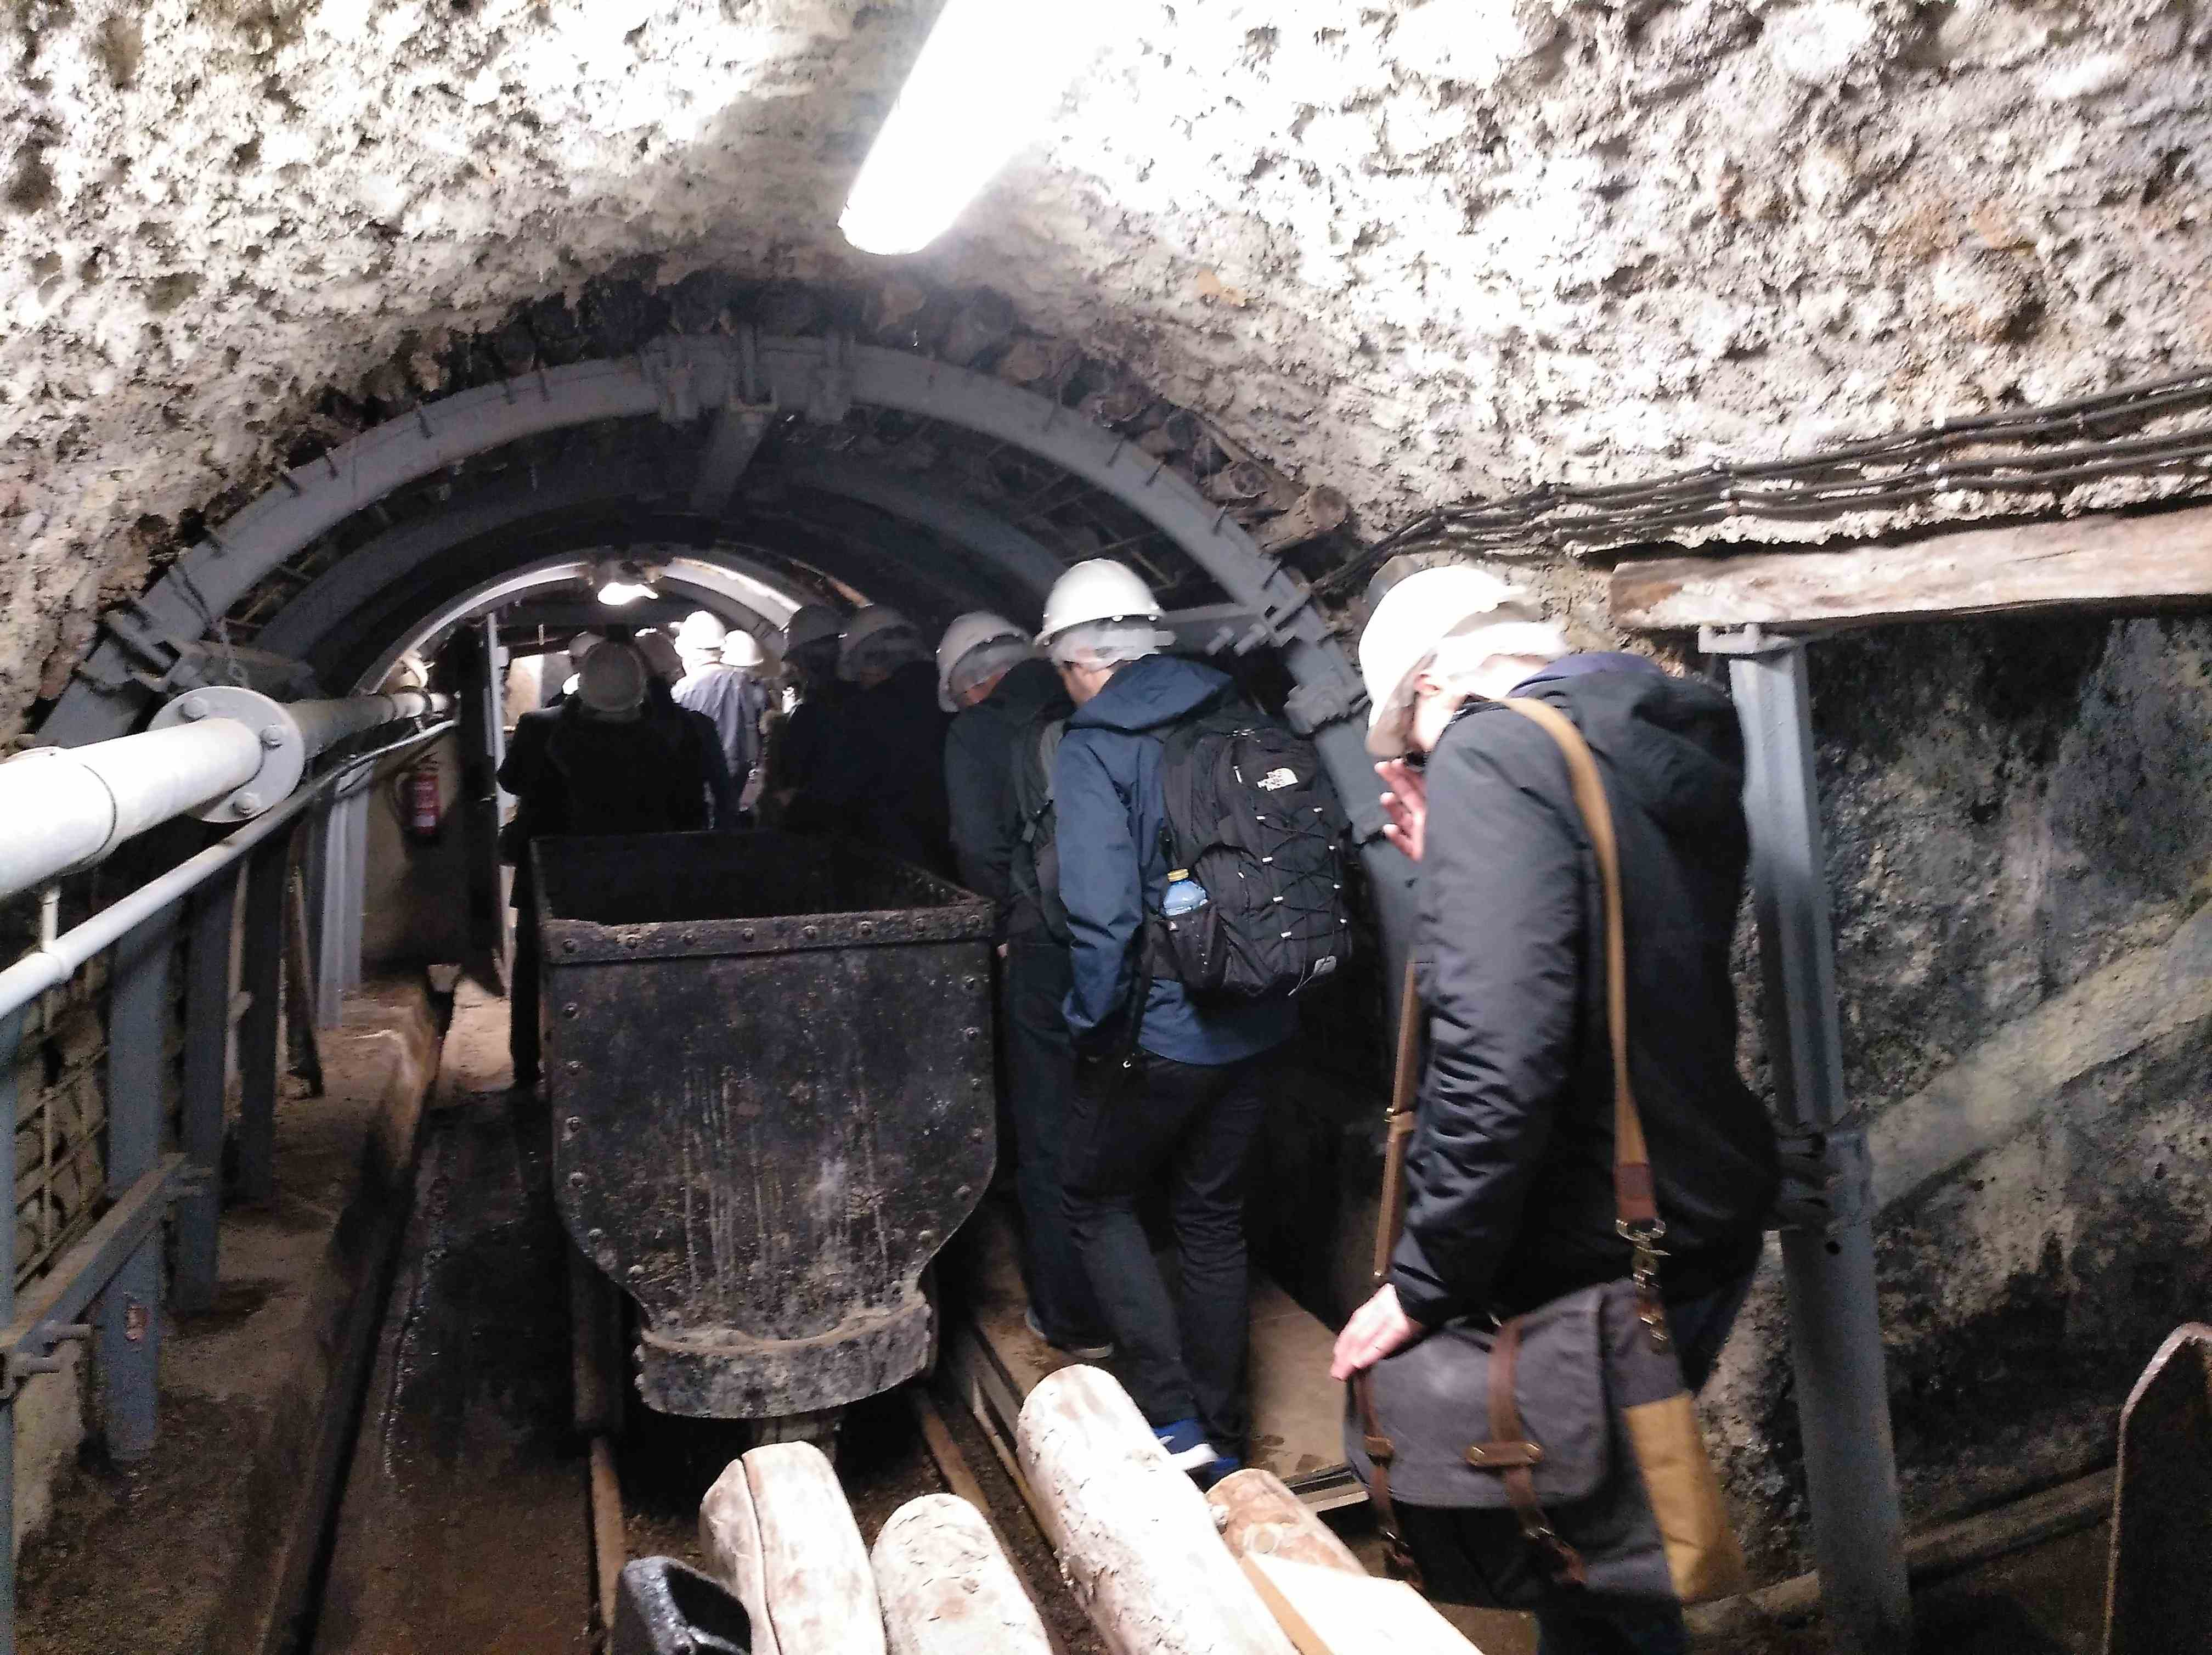
\includegraphics[width=.95\textwidth]{Mina}
	\label{fig:Mina}
	\caption{Visita a la mina Marcelo Jorissen - Fuente: Comité Organizador}
\end{figure}
\end{center}
%
\begin{center}
\begin{figure}
	\centering
		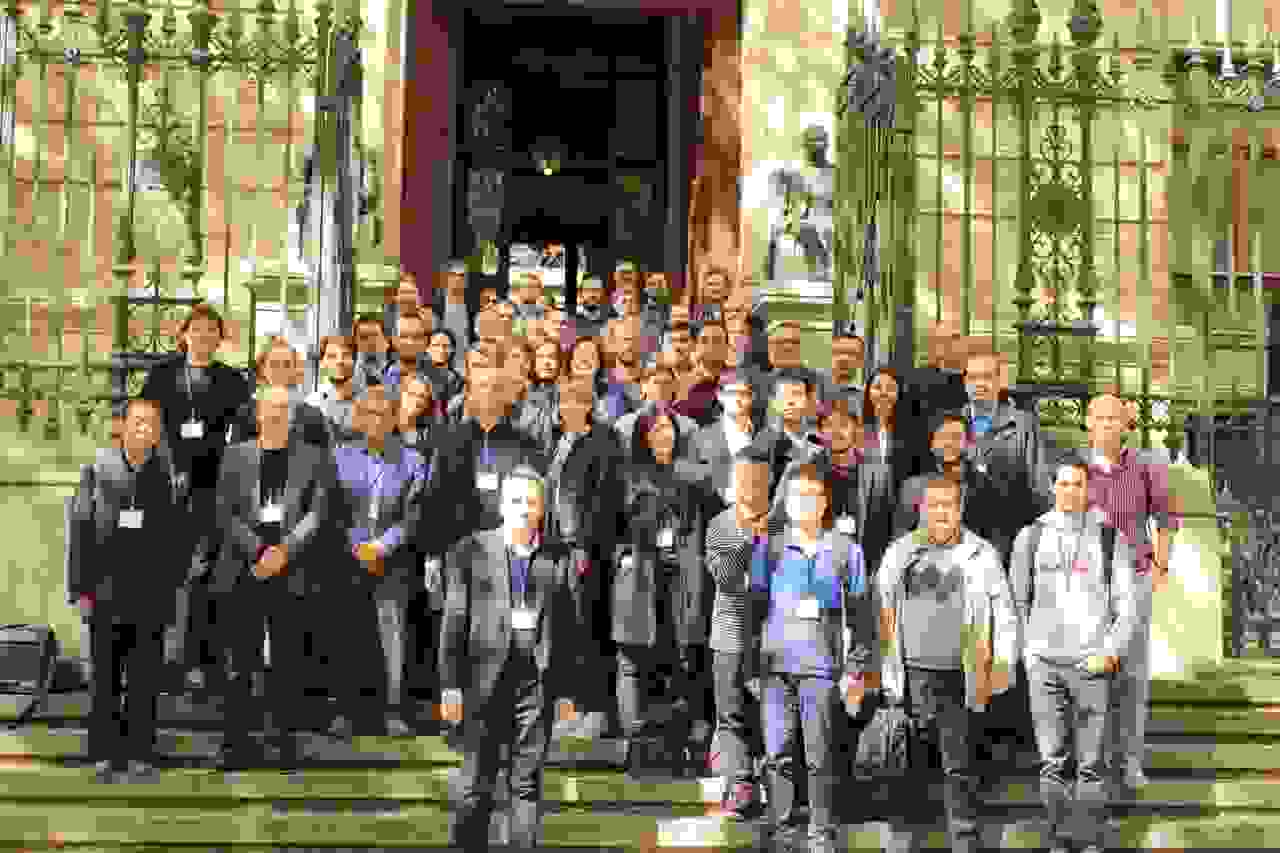
\includegraphics[width=.95\textwidth]{Group_Photo}
	\label{fig:GroupPhoto}
	\caption{Foto de grupo - Fuente: Comité Organizador}
\end{figure}
\end{center}
%
\begin{center}
\begin{figure}
	\centering
		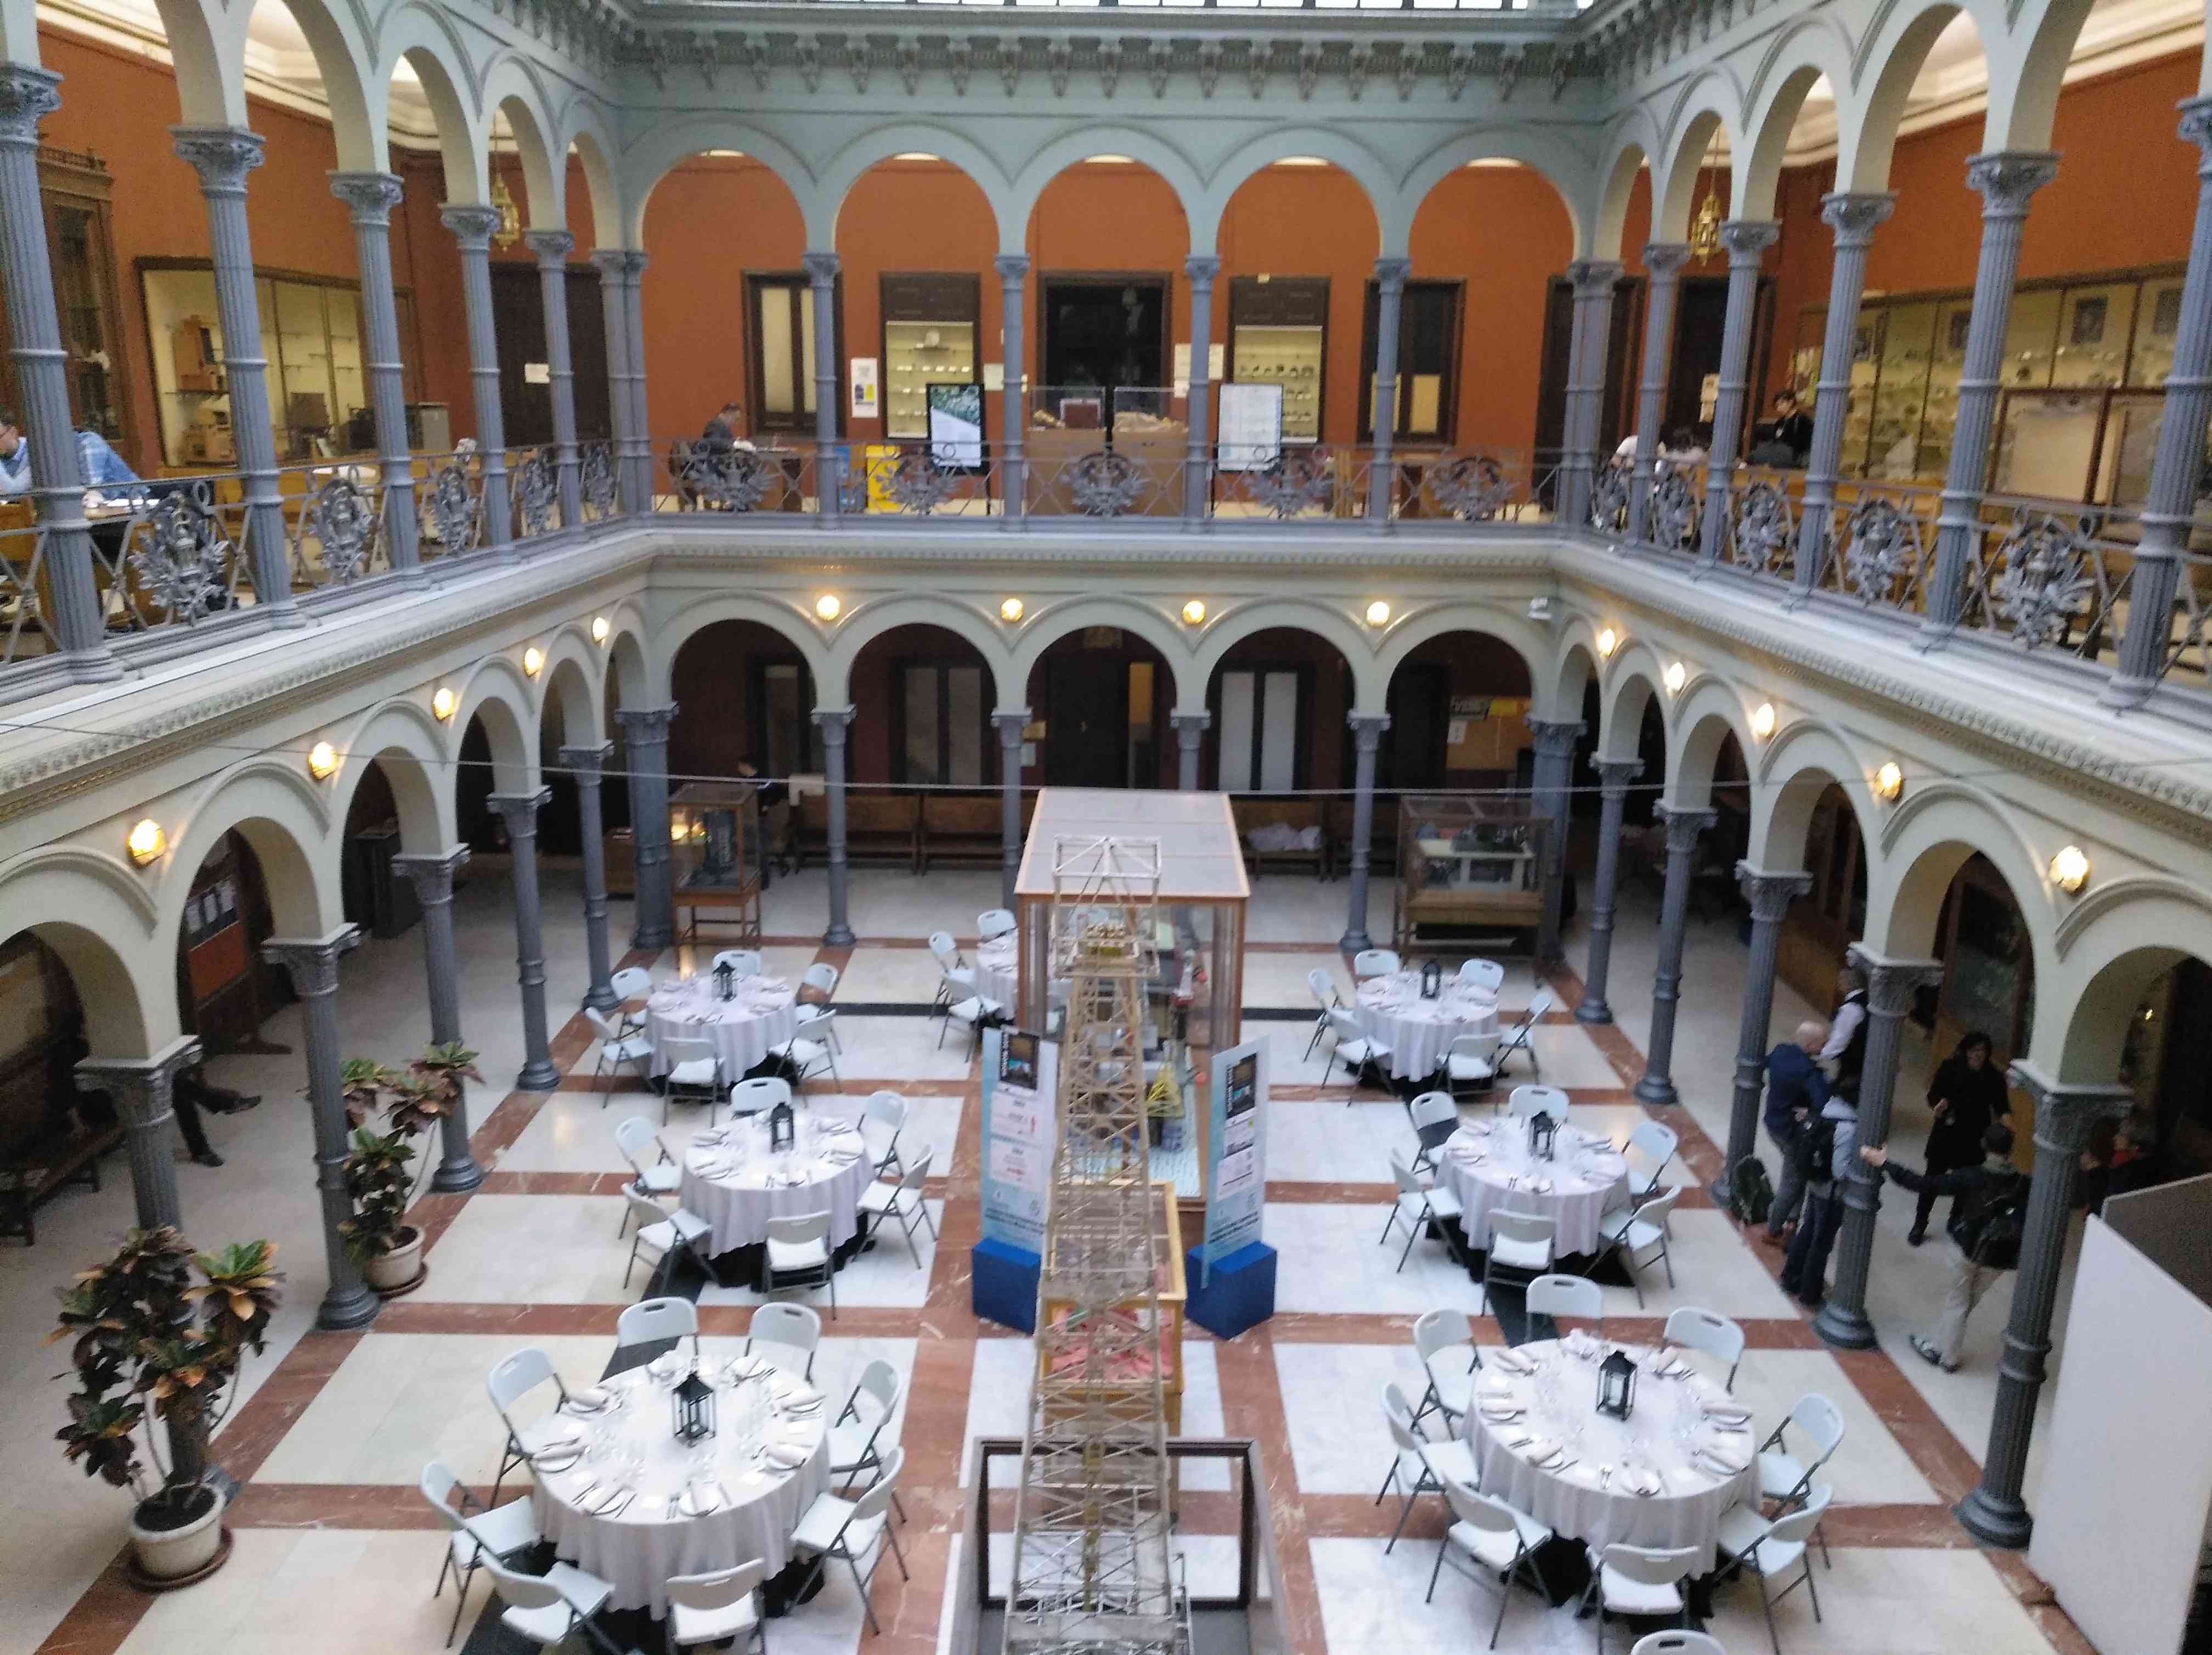
\includegraphics[width=.95\textwidth]{cena}
	\label{fig:CenaCong}
	\caption{Lugar de la cena del congreso: Patio de Columnas de la ETSIME - Fuente: Comité Organizador}
\end{figure}
\end{center}

%\begin{center}
%\begin{figure}
	%\centering
		%\includegraphics[width=.95\textwidth]{Cena_Congreso}
		%\includegraphics[width=.95\textwidth]{Cena_Congreso2}
	%\label{fig:Cenas}
	%\caption{Imágenes de la Cena del Congreso. - Fuente: Comité Organizador}
%\end{figure}
%\end{center}

\subsection{Clausura del congreso}
La clausura del congreso tuvo lugar después de la última charla en la que el presidente del Comité Organizador Local, Arturo Hidalgo, agradeció al Comité Organizador la oportuidad de celebrar esta nueva edición de HONOM en Madrid, así como a la Dirección de la Escuela Técnica Superior de Ingenieros de Minas y Energía de la Universidad Politécnica de Madrid por las facilidades dadas para que el congreso se celebrara en los locales de la Escuela. También agradeció a todos los participantes sus contribuciones, destacando su elevado nivel científico. Emplazó a todos para la próxima edición de HONOM, que tendrá lugar en Guimar$\tilde{a}$es (Portugal) en 2021.
\begin{center}
\begin{figure}
	\centering
		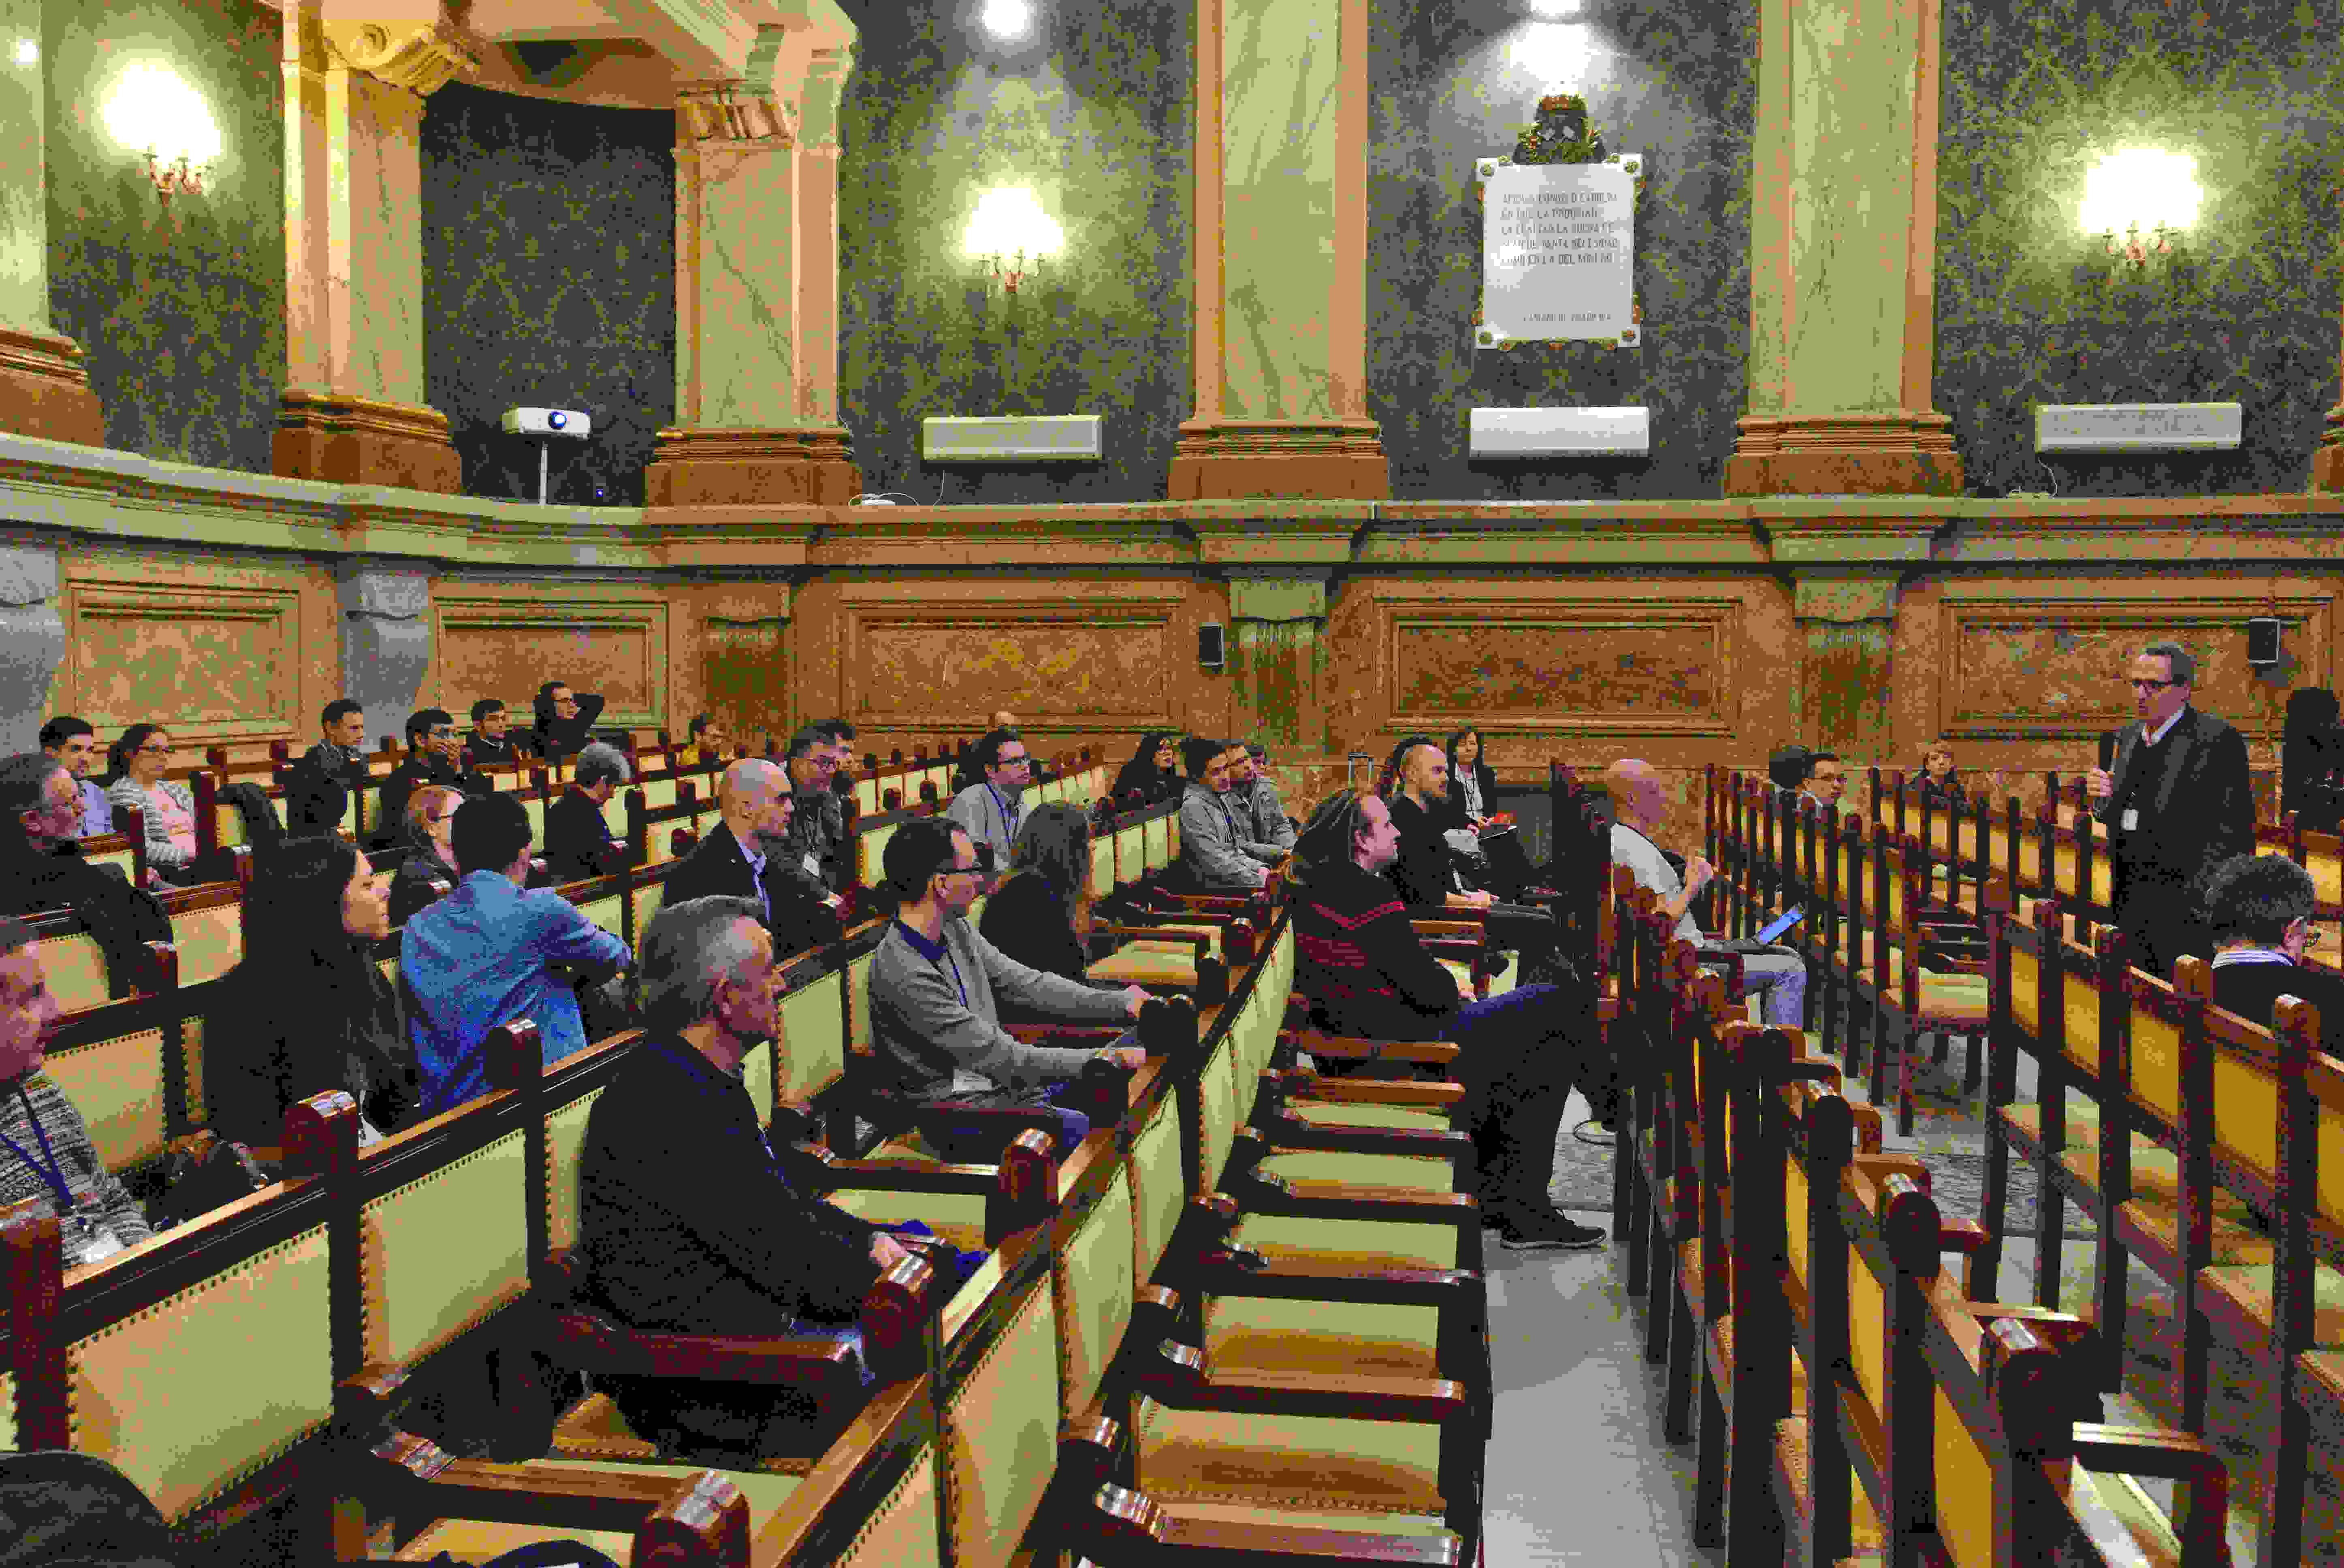
\includegraphics[width=.95\textwidth]{Clausura}
	\label{fig:Claus}
	\caption{Imagen de la clausura del Congreso. - Fuente: A. Baeza}
\end{figure}
\end{center}

\end{document}
